\documentclass{article}
\usepackage[utf8]{inputenc}
\usepackage{geometry}[margin=0.5in]
\usepackage{amsfonts}
\usepackage{amsmath}
\usepackage{amssymb}
\usepackage{physics}
\usepackage{braket}
\usepackage{amsthm}
\usepackage[english]{babel}
\usepackage{graphicx}
\usepackage{float}
\usepackage{mathtools}
\usepackage{algorithm2e}
\usepackage[hidelinks]{hyperref}
\usepackage[title]{appendix}
\usepackage{chngcntr}
\usepackage{cite}
\usepackage{lscape}

\theoremstyle{definition}
\newtheorem{definition}{Definition}[section]

\newcommand{\indep}{\perp \!\!\! \perp}

\usepackage{titlesec}
\titleformat{\section}[block]
  {\center}
  {\thesection .}
  {1em}
  {\MakeUppercase}
\titleformat{\subsection}[hang]
  {\center \it}
  {\thesubsection}
  {1em}
  {}

\usepackage{authblk}
\author[1]{Nico D'Angelo}
\author[2]{Kareem C Carr}
\author[3]{Sam Bessey}
\author[4]{Natallia Katenka}
\author[5]{M Elizabeth Halloran}
\author[8]{William C Goedel}
\author[9]{Samuel Freidman}
\author[2]{Brandon D L Marshall}
\author[6]{Ashley L Buchanan}
\author[1]{Eleanor J Murray}
\affil[1]{Department of Epidemiology, Boston University School of Public Health, Boston MA, USA
}
\affil[2]{Department of Biostatistics, Harvard TH Chan School of Public Health, Harvard University, Boston, MA, USA}
\affil[3]{Department of Epidemiology, Brown University School of Public Health, Providence, RI, USA}
\affil[4]{Department of Statistics, University of Rhode Island, Kingston, RI, USA}
\affil[5]{Department of Biostatistics, University of Washington, Seattle, WA, USA }
\affil[6]{Department of Pharmacy Practice, College of Pharmacy, University of Rhode Island, Kingston, RI, USA }
\affil[8]{Department of Epidemiology, Brown University School of Public Health, Providence, RI, USA}
\affil[9]{Department of Population Health, School of Medicine,
New York University, New York, New York, United States}

\renewcommand\Authands{ and }

\date{}

\begin{document}
\title{Causal Estimands for Network Effects Accounting for Network Structure}

\maketitle

[please check affilations \& amend or add as appropriate]

\newpage
\begin{abstract}
\textbf{Background:} Understanding networks can provide valuable information on transmitting or sharing knowledge, infection, resources, or other features among groups of individuals. Empirical networks are often difficult to ascertain exactly, especially for human populations. To address this, network-based simulation models were developed to aid in estimating patterns of outcomes that might be expected in real-world networks under a range of scenarios. Fundamentally, for all simulation models, these outputs can be considered estimates of counterfactuals,in that they describe what would have happened to the modeled population under a given set of inputs. However, if we want to interpret use these results to estimate causal effects in the real world, then we need to define the settings and assumptions under which comparisons of these simulated counterfactuals may be interpreted as estimates of real-world causal effects, and we need to define the target causal estimands of interest.\\
\textbf{Methods and Results:} We describe the unique challenges for estimating causal network effects and propose a set of causal estimands for estimating network effects under interventions. Using an example of pre-exposure prophlyaxis use as a preventive intervention for reducing HIV transmission, we demonstrate mathematically and via simulation modeling that these effects depend on network structure and that both the validity and the interpretation of causal network effects depend on features of the simulation design. We implement examples using Erdős–Rényi, Barabási–Albert, and Watts-Strogatz models and vary the inputs across univariate and multivariate parameter spaces. Our findings persist across model inputs. As predicted by our theoretical discussion, the model shows bias when the simulation is designed incorrectly, and this is minimized when either or both the simulation size or the number of simulations is large. \\
\textbf{Conclusions:} When causal network effects are of interest, simulation design should consider both the network structure and the specific details of the causal question. When the causal question of interest relates to the set of all possible networks with given input parameters, estimation requires the effect to be estimated on each network iteration. Each iteration of a simulated network should be subjected to each intervention set of interest, and comparisons should be made between results from sets of identical starting networks. If results for each intervention are instead combined across multiple network iterations before comparing between interventions, the causal network effect estimate is likely to be biased for finite numbers of iterations. This bias is a function of both network size and network connectivity and arises because of the flow of information between network connections.
\end{abstract}

\newpage


\section{Introduction}
When estimating causal effects, transmission and spillover both pose major challenges. Transmission occurs when the outcome of one individual can affect the outcome of another individual, and spillover occurs when the exposure of one individual can affect the outcome of other individuals \cite{halloran_dependent_2016}. These scenarios each violate a fundamental assumption required to estimate causal effects validly \cite{halloran_study_1991}. The Stable Unit Treatment Value Assumption (SUTVA) requires that the effect of treating a given individual is independent of the way in which treatment is delivered. Disease transmission (and other related forms of interference) inherently violate SUTVA since the effect of treating a given individual will now depend on the context of who else around them is exposed and/or has the outcome. 

A variety of paradigms have been proposed for defining causal estimands under interference so that well-defined questions that do not violate SUTVA can be asked. The most widely used of these is the \emph{dependent happenings} paradigm of Halloran et al.  \cite{halloran_study_1991} which defines community-level causal estimands. Other approaches include paradigms such as Ogburn \& Vanderweele's approach \cite{ogburn_causal_2014}, which focuses on describing whether interference arises from the exposure, outcome, or covariates of one individual affecting another individual, and the approach proposed by Cai et al. \cite{cai_causal_2021} which applies the logic of the dependent happenings paradigm to estimating infection timing within sero-concordant pairs under specific types of interference, and others \cite{forastiere_identification_2021,savje_average_2021}. 

Each of these three paradigms focuses on a somewhat different aspect of the causal question of interest. Together, they provide a useful roadmap for defining and estimating causal effects when interference is suspected, and all confounders are known and measured. However, the complexity of interference patterns means that obtaining sufficient sample sizes and data for estimating these effects is often prohibitively expensive and time-consuming and may require access to extremely sensitive personal information on research participants and their communities. As a result, many researchers rely on the use of simulation models to assess effects under interference \cite{murray_emulating_2021, buchanan_disseminated_2021,forastiere_identification_2021,buchanan_methods_2023}. Unfortunately, guidance on the design of simulation studies to estimate causal effects is sparse, particularly in network simulations.


Here, we describe an important aspect of network simulation studies that complicates the estimation of causal effects. We first review the existing paradigms for causal inference under interference and then describe an important design difference for network simulations that complicates the application of these paradigms. We consider the target estimands of interest for causal effects on networks when the empirical structure is known and then describe how using simulated networks can introduce bias into estimating these effects. 

In the present work, we focus on the setting of infection transmission when some members of the population receive a preventative intervention, such as vaccines or pre-exposure prophylaxis. We aim to answer the causal question: by how much would providing pre-exposure prophylaxis (PrEP) to 40\% of the uninfected population reduce HIV incidence compared ot providing PrEP to 20\% of the uninfected population? Our results are also generalizable to the effects of interventions to treat infection, interventions with post-exposure prophylaxis, or exposures that increase (rather than reduce) the susceptibility or vulnerability of uninfected individuals. 

\section{Notation}
Suppose we wish to estimate causal effects at the individual and community level of a program of pre-exposure prophylaxis (PrEP) to reduce susceptibility to HIV/AIDS for a network with $R$ nodes about which we have complete empiric data about all nodes and edge links in a real-world network. For simplicity, we simulate a study in which individuals livign with HIV/AIDs who report current or recent use of antiretrovirals and other medications are excluded. The use and effectiveness of medications could be incorporated in a similar simulation by including these as a time-varying covariate vector or incorporating them into the intervention of interest; however, doing so may add additional complexities due to the impact of treatment on future infection transmission risk.

Suppose there are $m$ individuals in the population who are infected with HIV/AIDS at baseline, so that the number of uninfected individuals is $N = R-m$. Then, let $A_{i}$ represent the PrEP status of a given uninfected individual, and $\mathbf{A} = (A_{1}, A_{2}, \ldots A_{N})$ represent the vector of PrEP status across the population network. The subvector $\mathbf{A_{-i}}$ represents the vector of treatment (PrEP) values for all currently uninfected individuals other than individual $i$.

In the following, we assume treatment status is randomized and determined via a Bernoulli individual assignment strategy such that, at any given time, all untreated and uninfected individuals within a population will initiate treatment according to the probability mass function: $\pi(\mathbf{A}, \alpha) = \prod_{i=1}^{N}{\alpha_{i}^{A_{i}}(1-\alpha)^{1-A_{i}}}$ and $0 < \alpha < 1$. 

For simplicity, we assume all previously treated individuals remain on PrEP treatment unless they become infected, and index the population treatment strategies with the parameter $\alpha$. For individuals who are HIV-infected, their value of PrEP treatment is zero. This assumption is not required -- we could equally assume that some proportion of infected individuals are undiagnosed and use prophylaxis despite already being infected, or we could consider individuals with infection who use treatment as a form of prophylaxis against transmission. Complex packages of interventions such as these would require careful simulation, and may face additional causal inference challenges, but the principles we discuss here will also apply.

Additionally, we denote the current infection status of any given individual with $Y_i$, the overall infection incidence in the network with $\mathbf{Y} = (Y_{1}, Y_{2}, \ldots, Y_{N})$, and the array of individual’s covariate values with  $\mathbf{C} = (C_{1}, C_{2}, \ldots, C_{R})$. Each of these can potentially change over time, although here we consider only static covariates. Individuals who are infected have an outcome value $Y=1$ from the time of infection. When assessing the incidence of infection, only individuals who's outcome value was 0 at the prior time step will be included in the estimation of the infection risk. Using this notation, we can define $Y_{i}(\alpha)$ as the counterfactual outcome that individual $i$ would have experienced had the network been intervened upon with strategy $A_i \sim Bern(\alpha)$. Similarly, we denote the average counterfactual outcome $E[Y(\alpha)] = E[Y_{i}(\alpha)]$, where the expectation of the counterfactual outcomes under strategy $\alpha$ is across individuals, $i$, as appropriate for the estimand of interest (see next section).

Finally, when referring to an alternative value of the intervention, network, or other parameter, we use the superscripts $*$, $**$, and $'$ on the original parameter symbol.

Using the above notation, the required causal inference assumptions for obtaining a valid estimate of the average counterfactual outcomes in the presence of interference for a population under a given intervention strategy $\alpha$, $E[Y(\alpha)]$, are as follows \cite{halloran_study_1991, hudgens_toward_2008, ogburn_causal_2014, tchetgen_tchetgen_causal_2012}:

%@article{tchetgen2012causal,
%  title={On causal inference in the presence of interference},
%  author={Tchetgen, Eric J Tchetgen and VanderWeele, Tyler J},
%  journal={Statistical methods in medical research},
%  volume={21},
%  number={1},
%  pages={55--75},
%  year={2012},
 % publisher={Sage Publications Sage UK: London, England}
%}%

\begin{enumerate}
\item Consistency under interference: $Y_{i}(\alpha)$ =$Y_{i}$ when $\mathbf{A} =\mathbf{a}$
\item 	Conditional exchangeability under interference: $Y_{i}(\alpha) \indep \mathbf{A} |\mathbf{C}$
\item Positivity under interference: $P({\mathbf A}= {\mathbf a} |{\mathbf C} = {\mathbf c}) \ge 0$ for all ${\mathbf a}$ in the support of ${\mathbf A}$ and for all ${\mathbf c}$ in the support of ${\bf C}$.
\end{enumerate}

An additional assumption that is often used to simplify inference in this setting is that of partial interference. Suppose the population of size $R$ is grouped into $j$ distinct subpopulations. Partial interference occurs when individuals can only affect the exposure and/or outcome of other individuals within their own subpopulation. That is, partial interference assumes that there is no interference between members of separate subpopulations. At one extreme, when $j$ = $R$, all individuals comprise their own subpopulation and the assumption is equivalent to assuming no interference occurs at all. At the other extreme, when $j$ = 1, then there are no separate subpopulations and the assumption is equivalent to that of full interference between any individuals. Importantly, in network simulations, the value of $j$ is often closer to 1 than to $R$, and the set of individuals within each subpopulation is defined by the specific pattern of links within the full network.

Finally, we will use the following notation for the network models. Let $G=(V,E)$ be a graph representation of a network, with vertex set $V$ and edge set $E$. Let $N$ denote the \textit{order} of $G$, equal to the cardinality of the vertex set $\vert V \vert$.

\section{Causal estimands with interference}
The dependent happenings paradigm defines four categories of causal estimands under interference. Briefly, these are the direct effect, the spillover (i.e., indirect) effect, the composite (i.e., total) effect, and the overall effect. Following the conventions of Hudgens \& Halloran \cite{hudgens_toward_2008} and Tchetgen Tchetgen \& Vanderweele \cite{tchetgen_tchetgen_causal_2012}, these four effects are defined as follows. 

\begin{definition}[Direct Effect]The direct effect is the benefit or harm experienced by each (uninfected) individual if they received the exposure versus if they had not, within a community context defined by intervention strategy $\alpha$. 
\end{definition}
Conditional on any confounders required to achieve exchangeability, the direct effect can be estimated by comparing the observed outcome distribution of the treated individuals within a given population to comparable untreated individuals within the same population. The direct effect contrasts counterfactuals under different individual treatment values within the same community context. The individual direct effect is defined by the following causal contrast for each treatment-eligible individual in the population under treatment strategy $\alpha$:
\begin{equation}\label{eq:1}
   DE_{i}\left(\alpha\right) = Y_{i}\left(\mathbf{a_{-i}}, a_{i} = 1\right) - Y_{i}\left(\mathbf{a_{-i}}, a_{i} = 0\right)	
\end{equation}
	
Where $Y_{i}(\mathbf{a_{-i}},a_{i})$ is the counterfactual outcome for individual $i$ when their treatment status is $a_{i}$ and all other individuals have treatment values $\mathbf{a_{-i}}$ following strategy $\alpha$. When treatment status has been randomized, the direct effect can be estimated by comparing the outcome values among the treated and untreated in the population. 

\begin{definition}[Spillover Effect] The spillover effect is the benefit or harm to each unexposed uninfected individual in a community if other individuals in the community had received exposure following intervention strategy $\alpha$ versus if those other individuals had received exposure following an alternate intervention strategy $\alpha*$. The individual spillover effect is:
\end{definition}

\begin{equation}\label{eq:2}
   SE_{i}\left(\alpha,\alpha*\right) = Y_{i}\left(\mathbf{a_{-i}}, a_{i} = 0\right) - Y_{i}\left(\mathbf{a_{-i}*}, a_{i} = 0\right)	
\end{equation}

The spillover effect can be estimated, under the causal inference assumptions above, by comparing the observed outcome distribution among untreated individuals in a population with a particular treatment allocation strategy to that of untreated individuals in a comparable population with a different treatment allocation strategy. The spillover effect thus contrasts counterfactuals under a constant treatment status within different community contexts, where $\alpha$ and $\alpha*$ are the two intervention strategies being compared and $\mathbf{a_{-i}}$ and $\mathbf{a_{-i}}*$ represent the pattern of treatment for all individuals other than individual $i$ under each intervention strategy.

	
\begin{definition}[Composite effect]The composite effect is the benefit or harm experienced by eligible individuals if they had received exposure under a particular community context defined by the intervention strategy compared to what their experience would be if they did not receive exposure and their community context followed a different intervention strategy.
\end{definition}

\begin{equation}\label{eq:3}
   CE_{i}\left(\alpha,\alpha*\right) = Y_{i}\left(\mathbf{a_{-i}}, a_{i} = 1\right) - Y_{i}\left(\mathbf{a_{-i}*}, a_{i} = 0\right)	
\end{equation}

When the causal inference assumptions hold, the composite effect can be estimated by comparing the outcome distribution among treated individuals, in a population with a given proportion of individuals who receive treatment, to the experience of untreated individuals in a comparable population with some different proportion of treated individuals. The composite effect contrasts counterfactuals where both the individual treatment status and their community context are altered. The composite effect can be decomposed into the direct and spillover effects.

\begin{definition}[Overall effect] The overall effect is the benefit or harm to each individual in the community, if  eligible individuals had received the exposure under intervention strategy $\alpha$ versus if eligible individuals had received the exposure according to an alternate intervention strategy $\alpha*$.
\end{definition}

\begin{equation}\label{eq:4}
   OE_{i}\left(\alpha,\alpha*\right) = Y_{i}\left(\alpha\right) - Y_{i}\left(\alpha*\right)	
\end{equation}

The overall treatment effect can be conceptualized as the community-level counterfactual outcome and contrasts the counterfactual outcomes for the entire community under different community contexts. It can also be viewed as a weighted average of the effect for each individual of changing their individual treatment status and community context in the way defined under the intervention strategies being compared, where the weights represent the frequency of treatment-context change types in the population.


\section{Causal estimands on networks with interference}
For all four of the above individual estimands, we can also define individual average estimands by taking the weighted average over all possible contacts the index individual can have. Since the actual contacts may not be known, we can also estimate this via weighting over the distribution of treatment of possible contacts. We can similarly define population (or subpopulation, if assuming partial interference) average estimands by further aggregating across all relevant index individuals. Typically, we focus on these average estimands when relying on randomized trial, observational, or simulation-based studies \cite{halloran_dependent_2016, murray_emulating_2021, buchanan_disseminated_2021}.
%Halloran and Hudgens Curr Epidemiol Rep. 2016 Dec; 3(4): 297–305%
However, investigators studying infectious diseases or other transmissible exposures are increasingly interested in using network-based simulation models. If the network under study is an empirical network with a known structure of members and connections, then the previously described approaches may be appropriate since the contacts for each individual have occurred in the past and are essentially a fixed property of the network structure. An important caveat of these estimates is that they may not generalize to other real-world networks with different structures (including future iterations of the measured network). We can thus define the network-based dependent happening estimands as conditional on the specific network of interest as follows. 

\begin{definition}[Network-specific overall effect] The network-specific overall effect is the average benefit or harm to the whole community if some or all individuals had received the exposure under intervention strategy $\alpha$ versus if individuals had received the exposure according to the intervention strategy $\alpha*$ for a given network realization $G=g$ (Equation \ref{eq:5}).
\end{definition}

For simplicity, assume for the moment that the network structure is static over time and that the observed network $G =g$ is a single realization from a distribution of possible network structures defined by some (potentially unknown) set of network parameters. We could then write the overall effect of a treatment strategy on the network $G=g$ as:

\begin{equation}\label{eq:5}
   OE_{g}\left(\alpha,\alpha* |G=g \right) = E[Y_{i}\left(\alpha|G=g\right) - Y_{i}\left(\alpha*|G=g\right)].	
\end{equation}

We could similarly define network-specific direct effects, spillover effects, and composite effects.

Now consider the case where we are interested in estimating causal effects for a set of $q$ multiple, different real-world networks. In this case, we may not be interested in the network-specific effects, but rather in the effects of the intervention strategies averaged across all $q$ networks. That is, we are interested once more in the direct, spillover, composite, and overall effects as originally defined \cite{hudgens_toward_2008} (Equation \ref{eq:4}). Given existing networks and the definition of the network-specific effects, it is relatively straight-forward to see that the population average causal effect across networks could be obtained from the simple mean of all network-specific average causal effects, such that, for example the overall effect could be estimated by:

\begin{equation}\label{eq:6}
   OE\left(\alpha,\alpha* \right) = \frac{\sum_{g=1}^qE\left[Y_{i}\left(\alpha|G=g\right) - Y_{i}\left(\alpha*|G=g\right)\right]}{q} \text{   
 }\forall g \in G.	
\end{equation}


Often, however, the exact network is not well-described, and instead, only some set of defining network parameters are known. Investigators must now simulate a range of potential networks that follow these distributions and use these simulated networks to estimate causal effects. If we were able to simulate every possible realization of a given set of network parameters, then we could use the average counterfactual outcomes across all realizations to estimate the average causal effects using Equation \ref{eq:6}. However, simulating all possible network realizations is typically computationally prohibitive, and even simulating an extremely large number of realizations may be computationally infeasible. Since we are limited to assessing only a finite number of network realizations, we can instead estimate the population average effects by taking the weighted average of network-specific effects, where the weights represent the likelihood of a particular network structure:

\begin{equation}\label{eq:7}
   OE\left(\alpha,\alpha* \right) = \sum_{g=1}^qE\left[Y_{i}\left(\alpha|G=g\right) - Y_{i}\left(\alpha*|G=g\right)\right]P\left[G=g\right].	
\end{equation}

The probability of each network realization can be derived from the input network parameters or computationally by simulating multiple network realizations given the network-defining parameters and averaging over simulation runs. Note that in this discussion, we are assuming the network realizations are selected at random from all possible realizations under the input parameters. If network realizations were simulated conditional on some covariates, these should be included in the weights.

In contrast, the network-specific effects need to be carefully simulated. One standard approach to estimating network effects is to resimulate the network every time the simulation is run, so that the counterfactual outcomes are generated on a newly simulated network.  This approach can be computationally more efficient since the structure of the network does not need to be retained between estimates. However, for finite simulation sizes, this approach will introduce bias into the effect estimate. 

If there is no limit to our capacity to simulate network realizations, then the method of simulating network realizations is irrelevant to the causal estimation process since we are summing each set of weighted counterfactuals over all $q$ versions of $G$. But realistically, we will often be restricted to a finite number of fewer than $q$ simulation runs. In this case, resampling the network for every estimate will result in the set of network realizations $G=g$ differing from the set of network realizations $G=g*$. The result is that our estimator becomes Equation \ref{eq:8}.

\begin{equation}\label{eq:8}
   OE\left(\alpha,\alpha* \right) = \sum_{g=1}^{q_1}E\left[Y_{i}\left(\alpha|G=g\right)\right]P\left[G=g\right]- \sum_{g=(q_1 +1}^{q_2}E\left[Y_{j}\left(\alpha*|G=g*\right)\right]P\left[G=g*\right].	
\end{equation}
where $q_1+q_2 < q$ is the total number of network realizations modeled, and $i$ and $j$ are the indices for nodes on each set of network realizations.

While Equation \ref{eq:8} still involves contrasting counterfactual outcomes, it is not actually guaranteed to estimate any causal effect. In fact, since the purpose of using a network simulation is that the structure of the network links is expected to affect the resulting outcome distribution, Equation \ref{eq:8} is generally guaranteed to be biased because, in epidemiologic terms, network structure is a possible effect modifier \cite{buchanan_spillover_2022} and the contrasting counterfactual outcomes are conditional on different subsets of network structures.

When the goal is to estimate causal effects using networks, and when the number of simulation runs is finite (and especially when the number of runs is small), each network realization should be retained as the starting point for simulating the counterfactual outcome under every intervention strategy being evaluated. Then, the network-specific effect can be estimated conditional on each $G=g$ before averaging across the set of simulated realizations. 

In the remainder of the paper, we show with a simple worked example, as well as with simulations, that bias does happen when the simulation approach uses Equation \ref{eq:8} instead of Equation \ref{eq:7}. In the simulations, the bias occurs when we randomly regenerate the network for every counterfactual estimation and decreases with increasing network size or simulation numbers. We also describe the conditions under which this bias is likely strongest for a given network.

\section{A simplified, illustrative example of the problem}
Suppose we are interested in estimating the population-level causal effects of a program to distribute PrEP to individuals potentially at risk of acquiring HIV/AIDS. Assume that no individuals in our population are currently receiving, or have ever received, PrEP. Then suppose that $m$ individuals are living with HIV/AIDS, and $N = R-m$ individuals are uninfected at baseline (Figure \ref{fig: Figure 2}). If we were to follow this population over time, without distributing PrEP, we would likely observe transmission of infection over time, such that the prevalence of HIV infection $m_t/R$ increases and the proportion of uninfected individuals $N_t/R$ decreases. 

\begin{figure}[H]
    \centering
    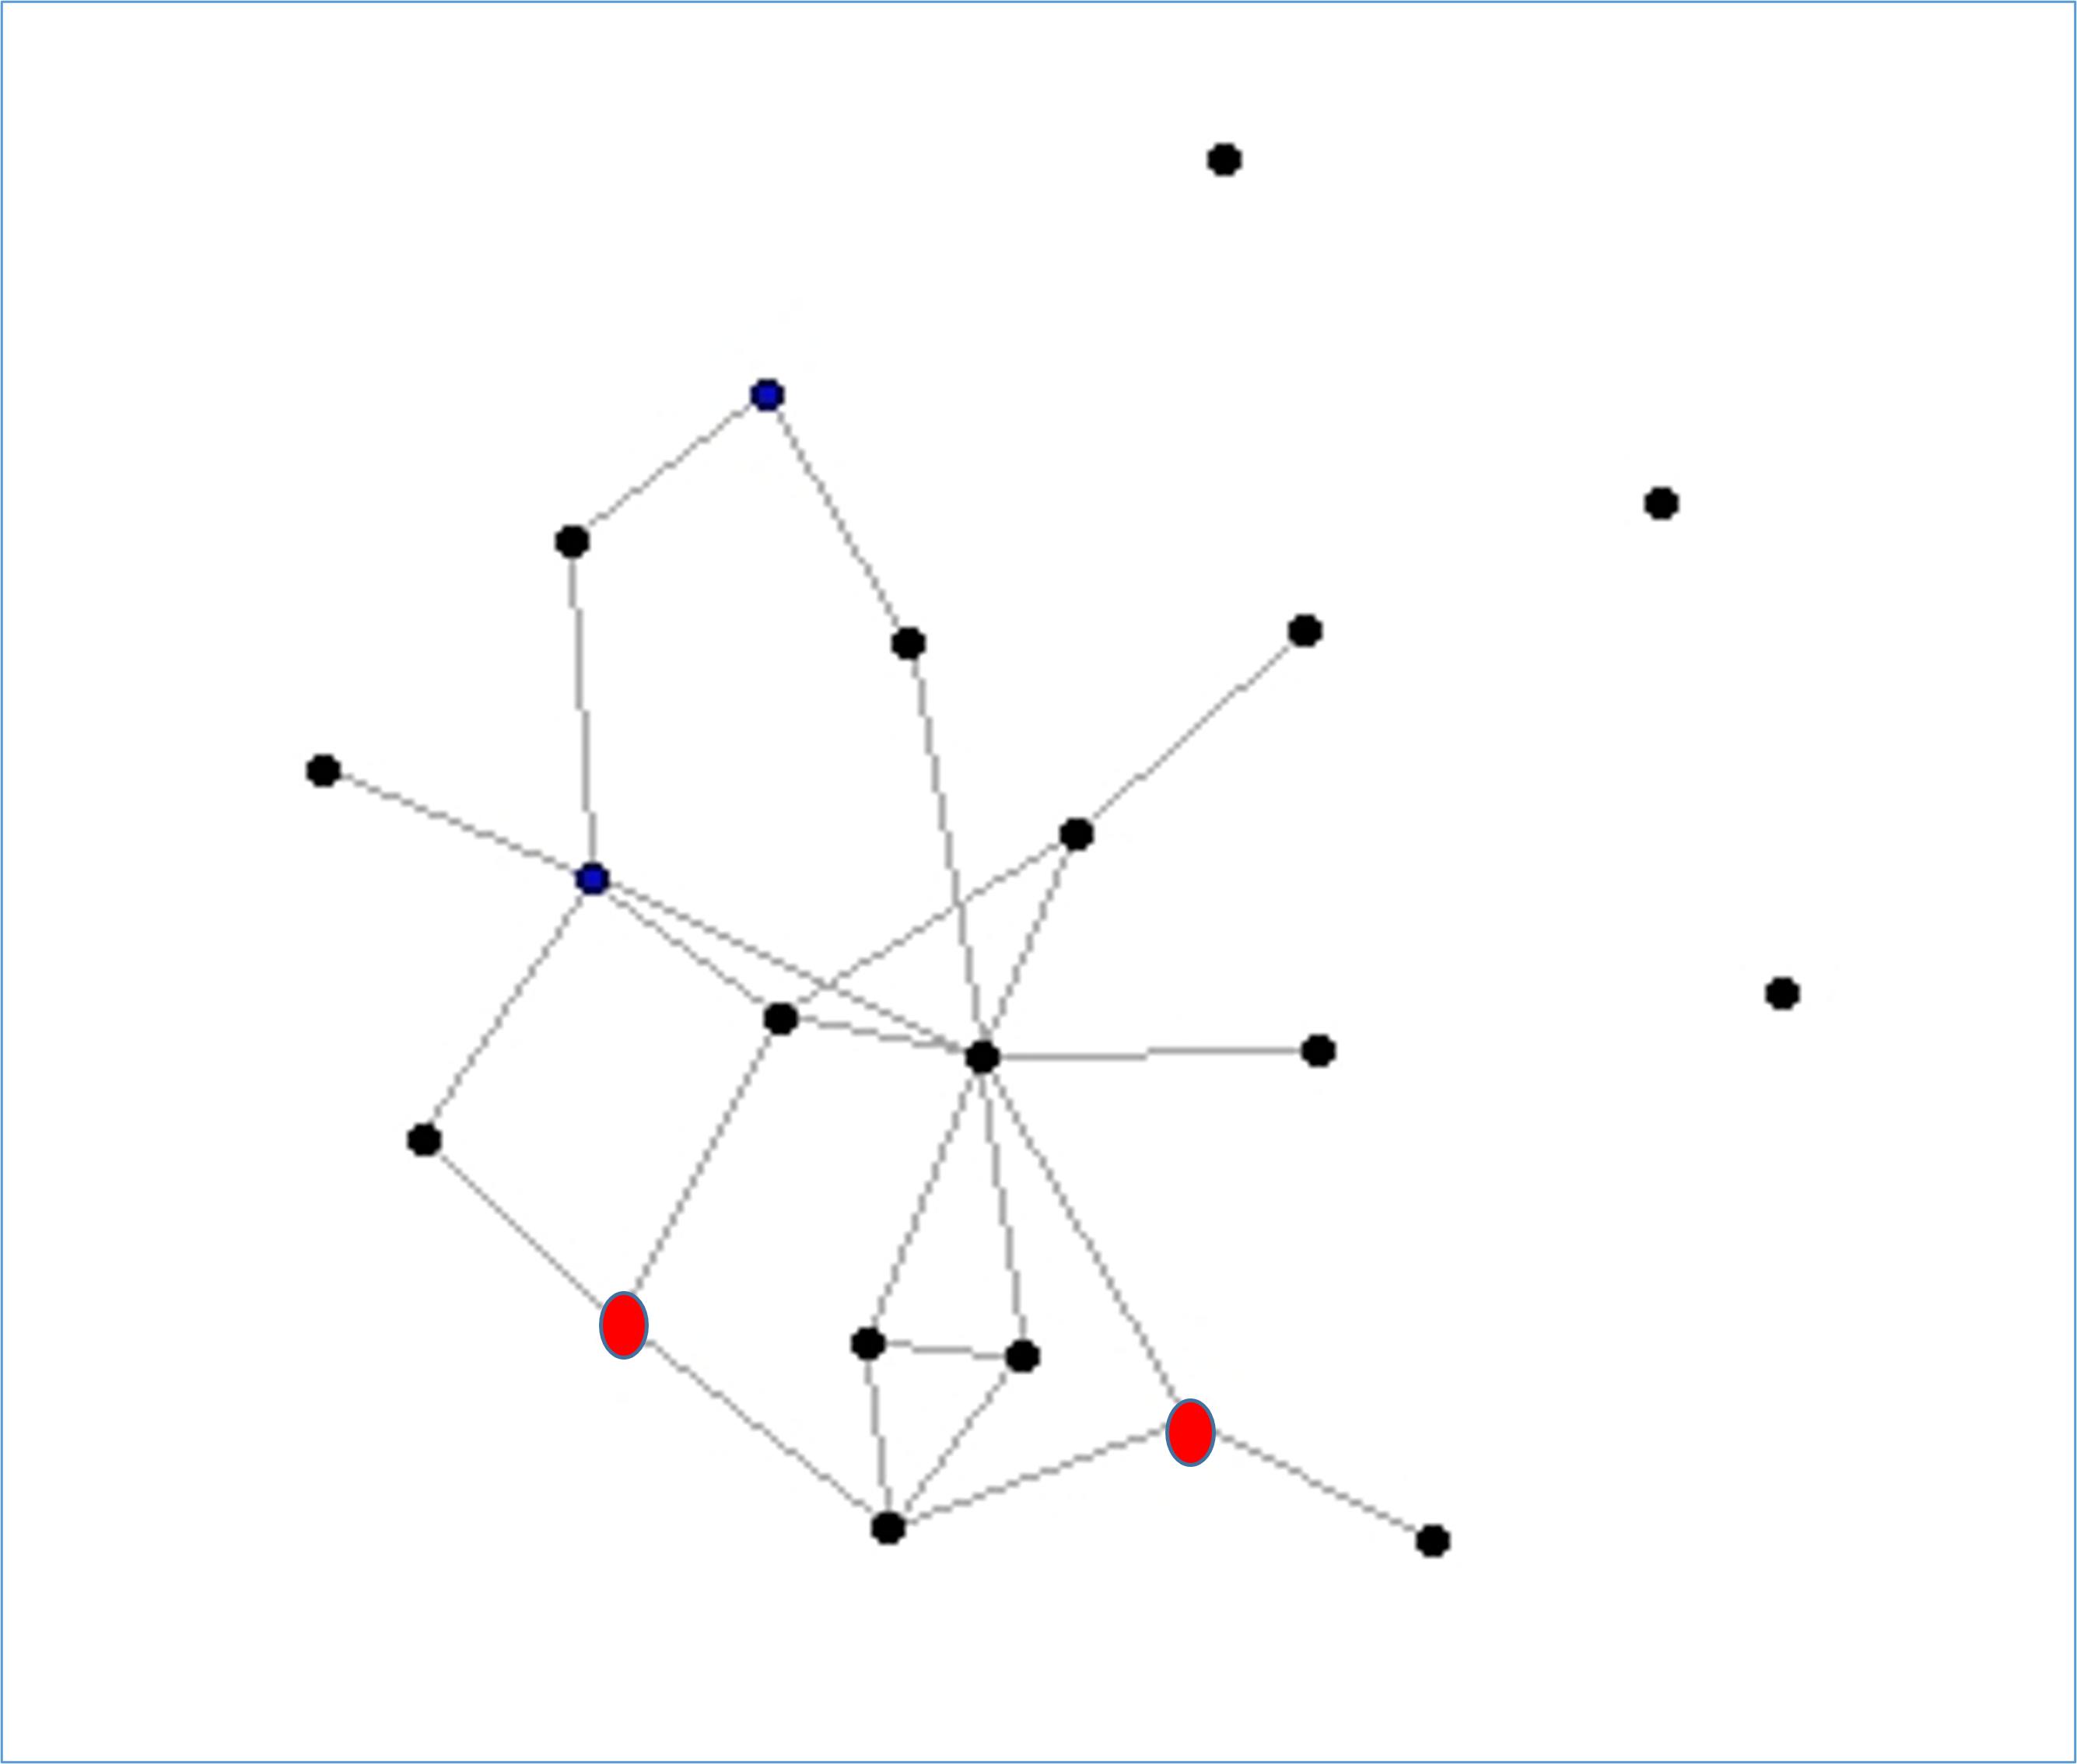
\includegraphics[scale=0.5]{Original Figures/Network Example 1.png}
    \caption{One possible realization of a simple network where $m = 2$ individuals are living with HIV (red nodes), and $N=R-m = 18$ individuals are currently uninfected (black nodes). The edges represent sexual partnerships.}
    \label{fig: Figure 2}
\end{figure}

Suppose that the network links represent sexual partnerships. We can see from Figure \ref{fig: Figure 2} that only a subset of individuals, $n$, have sexual partners living with HIV/AIDS at baseline (in this realization of the network, $n=5$ direct partnership contacts). For these $n$ individuals, their risk of acquiring HIV will be some probability $p$ between 0 and 1. On the other hand, in the first time step, the remaining $N-n$ uninfected individuals who have no sexual partners living with HIV/AIDS (here, 13 individuals) will have a probability of acquiring HIV equal to 0 (ignoring other transmission routes for simplicity). Thus, for each uninfected individual, their probability of infection will be either $p_i$ or 0, while the average risk of infection in the population overall after a one-time step could be estimated by:
\begin{equation}\label{eq:9}
E[\hat{Y}\left(\mathbf{\alpha} =0|G=g\right)]= \frac{\sum_{i=1}^{n}p_{i}}{N} = \frac{n\bar{p}}{N}.
\end{equation}

Now consider an intervention strategy delivered to this same population such that some proportion $k/N$ uninfected individuals receive PrEP.  Following the intervention, the $n$ individuals who have a sexual partner living with HIV/AIDS will have either the same probability $p$ of infection as before or a lower probability $p'$ of infection if they are receiving PrEP, since PrEP aims to prevent infection following infectious exposure. 

Among the individuals with no partners living with HIV/AIDS, the risk of infection will remain unchanged at 0. If our intervention strategy happens to only deliver PrEP to this latter group, the average risk of infection in the population will remain at $n\bar{p}/N$ regardless of the proportion of individuals given PrEP. On the other hand, if we had distributed PrEP only to individuals with infectious contacts, the average risk of infection would have been reduced. When $n=k$ and PrEP is distributed to only those with infectious contacts, the average population risk is $kp'/N$.

Why does this matter? Our goal is to estimate how the HIV infection risk changes when we do versus do not deliver the intervention strategy to this network. But we can see from the above that the intervention “give PrEP to $n$ individuals” can be implemented in a range of ways, resulting in a range of possible counterfactual outcomes for infection under the intervention strategy even when the network is the same. In general, we would expect the effect of "give PrEP to $n$ individuals" compared to "give PrEP to no individuals" to be bounded between 0 and $(kp'/N - kp/N)$ for any single network structure in any single time step, and the population average overall effect will then depend on the distribution of possible treatment allocations on the network under the intervention strategy. 

Figure \ref{fig: Figure 3}  depicts one possible treatment allocation on the network in Figure \ref{fig: Figure 2} under the strategy is "give PrEP to 10\% of eligible individuals". In this image, two uninfected individuals have been randomly assigned to receive PrEP. In this particular realization of the network intervention, it happens that all individuals assigned to PrEP are not exposed (i.e., have no sexual partnerships with HIV-positive individuals). For those individuals, PrEP does not change their initial probability of HIV infection; and for the entire network, the addition of PrEP does not change the expected incidence of infection over the next time step.

\begin{figure}[H]
    \centering
    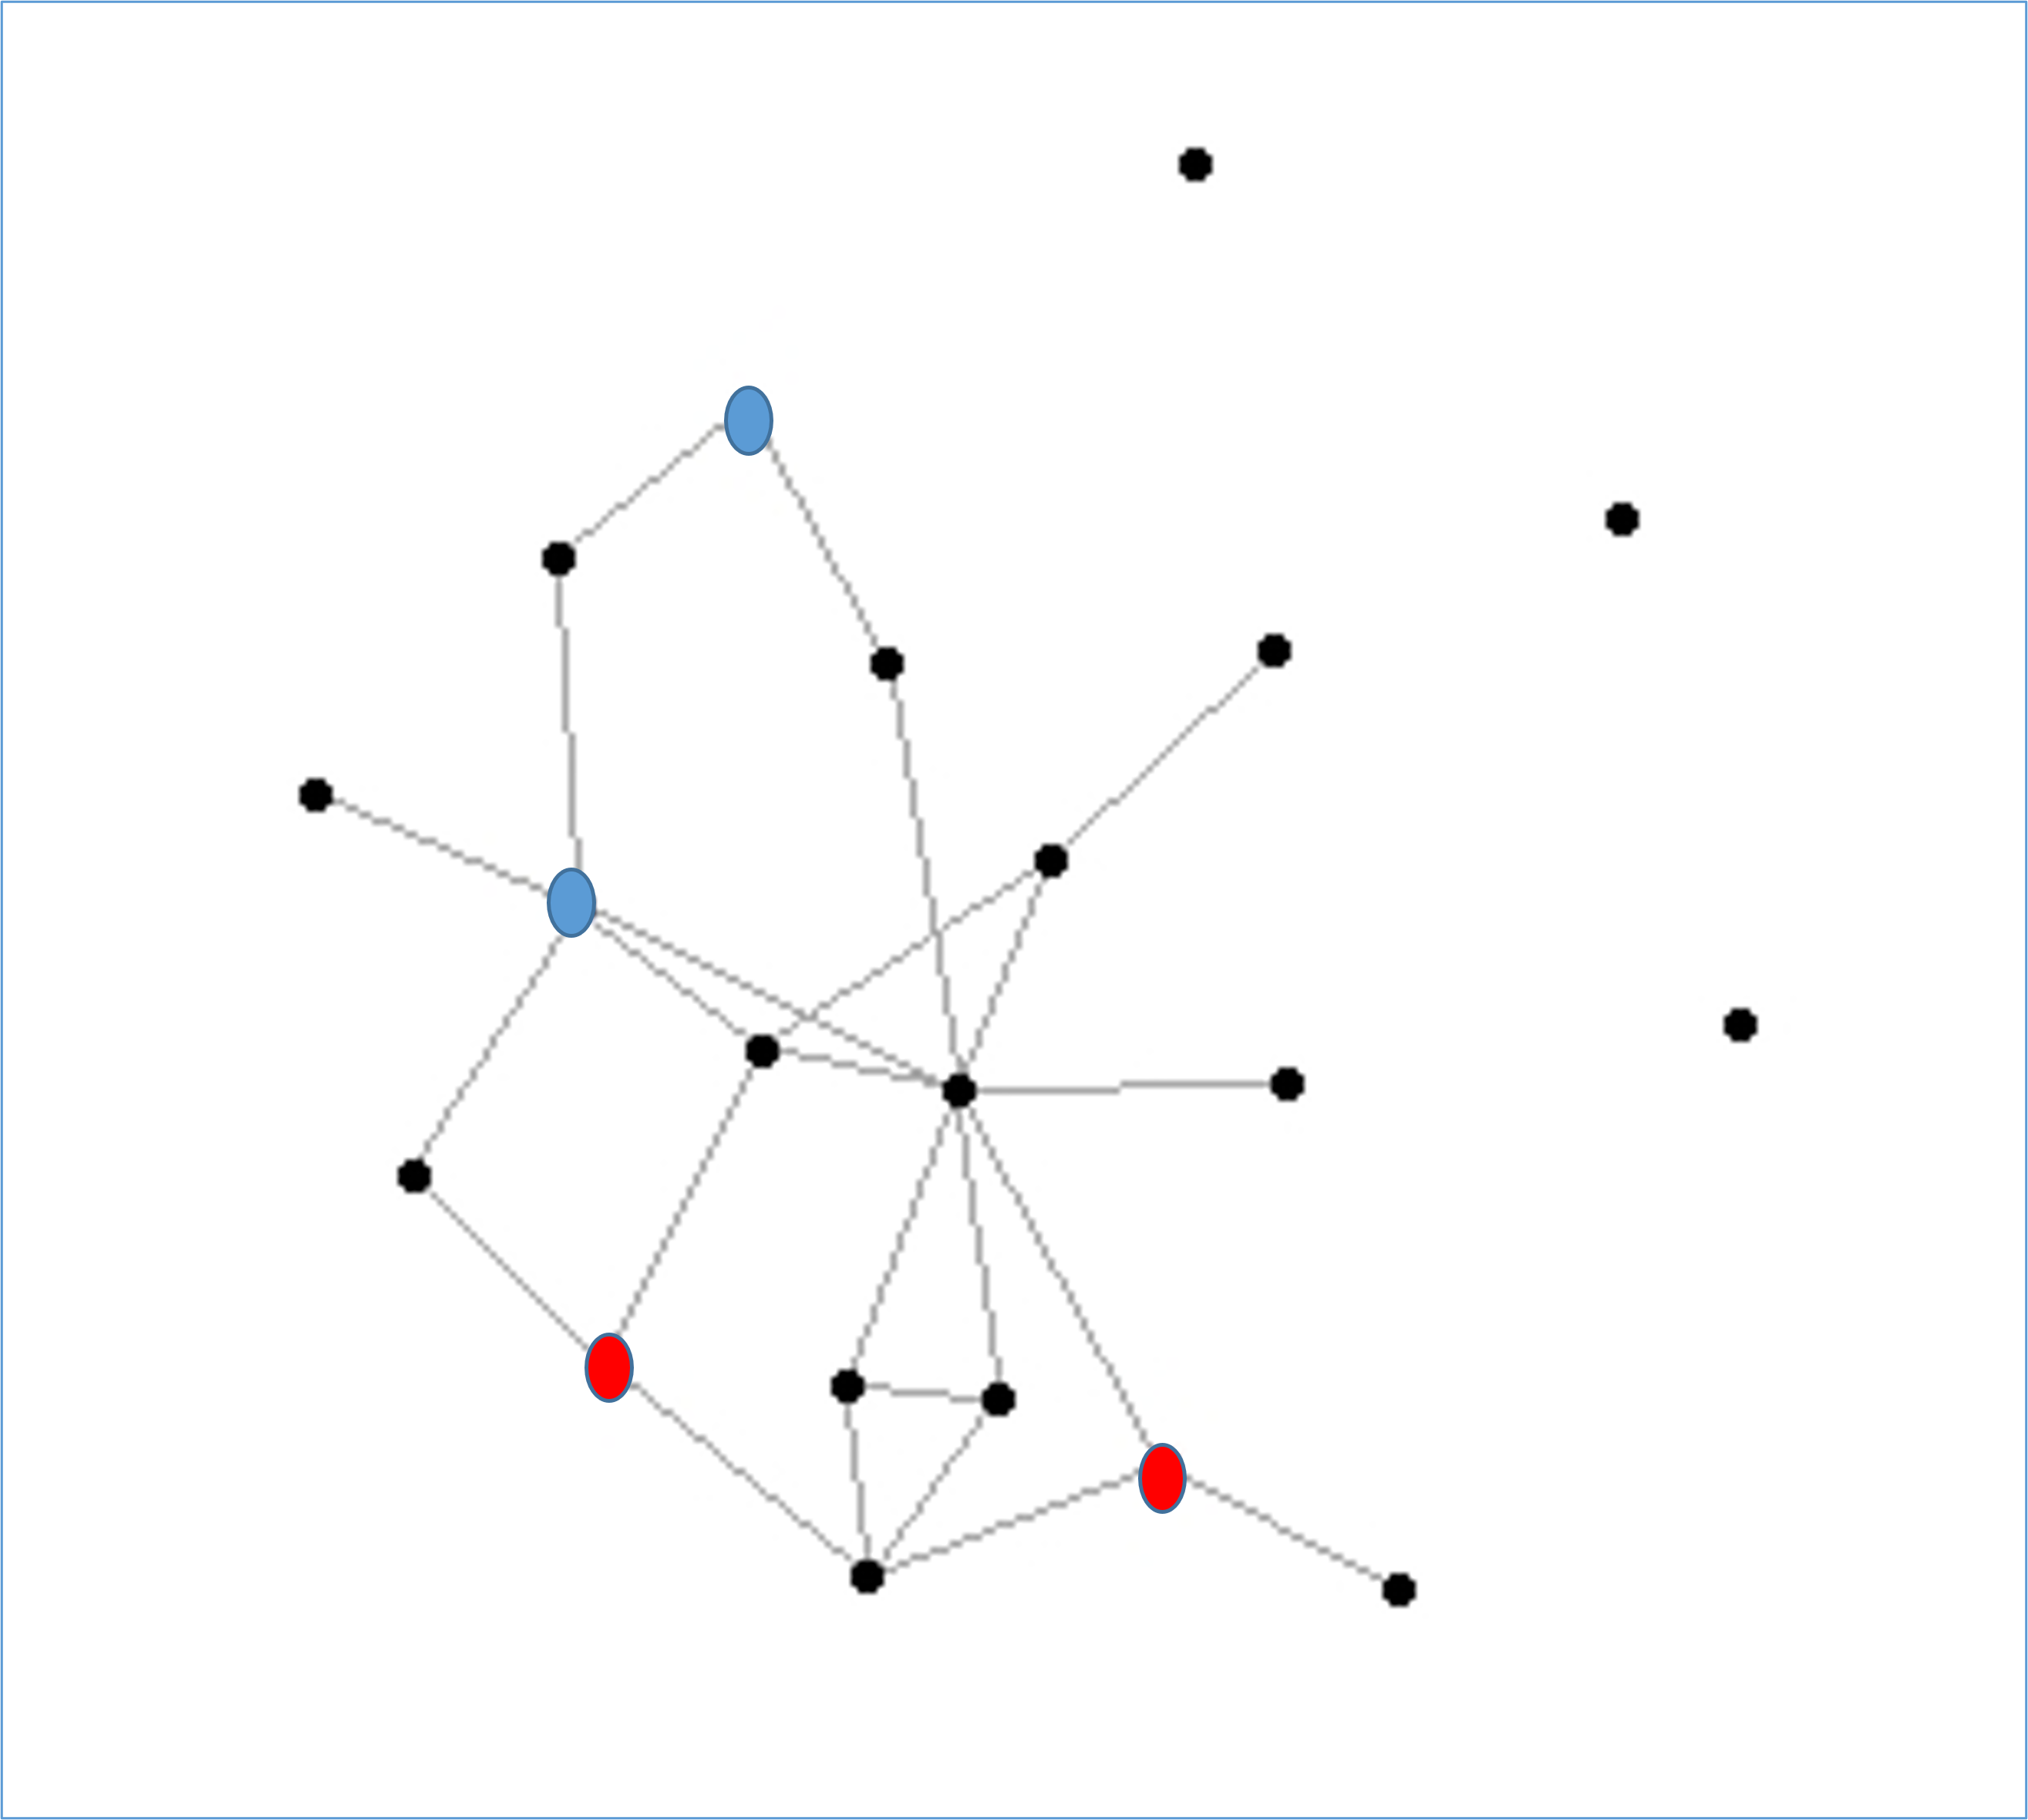
\includegraphics[scale=0.5]{Original Figures/Network Example 2.png}
    \caption{Random PrEP assignment to the network with 10\% coverage of uninfected individuals. The 2 blue nodes represent uninfected individuals assigned to PrEP; red nodes represent individuals living with HIV; black nodes represent individuals without HIV and not assigned to PrEP.}
    \label{fig: Figure 3}
\end{figure}

After PrEP assignment in Figure \ref{fig: Figure 3}, the counterfactual outcome over the next time step can be estimated using Equation \ref{eq:9} as follows:

\begin{align}
\begin{split}
E[Y\left(\mathbf{\alpha}|G=g\right)] & = \frac{\sum_{i=1}^{n}(p_{i})}{N}  \\ 
& = P\left(Y|PrEP = 0, Contact = 1\right)P\left(PrEP = 0, Contact = 1\right)  \\ \nonumber
& +P\left(Y|PrEP = 0, Contact = 0\right)P\left(PrEP = 0, Contact = 0\right)  \\ \nonumber
& +P\left(Y|PrEP = 1, Contact = 1\right)P\left(PrEP = 1, Contact = 1\right) \\ \nonumber
&  +P\left(Y|PrEP = 1, Contact = 0\right)P\left(PrEP = 1, Contact = 0\right) \\ \nonumber
 &=  \frac{5}{18}*p_1 +  \frac{11}{18}*0 +\frac{0}{18}*p_2 +  \frac{2}{18}*0 \\ \nonumber
 &=\frac{5p_1}{18}  \nonumber
\end{split}
\end{align}

where $p_1 = P(Y|PrEP=0,Contact=1)$, $p_2 = P(Y|PrEP=1,Contact=1)$.

In the network realization simulated in Figure \ref{fig: Figure 3} no individuals have both PrEP and infectious sexual contact, so the value of $p_2$ does not matter here. Likewise, individuals who have no infectious contacts, regardless of PrEP status, have no probability of infection (in the first time step). Therefore, the outcome at the end of the first step will be entirely driven by the probability of transmission with an infectious contact and no PrEP, $p_1$.

Now, assume we are interested in estimating the causal effect of increasing PrEP coverage in networks with these parameters. A common network simulation approach would be to generate a new network with the same input parameter distributions as the original network, but in which the PrEP coverage differs -- say 20\%. Figure \ref{fig: Figure 4} gives an example of 20\% treatment allocation on a new randomly generated network using the same input distributions as the prior examples.

\begin{figure}[H]
    \centering
    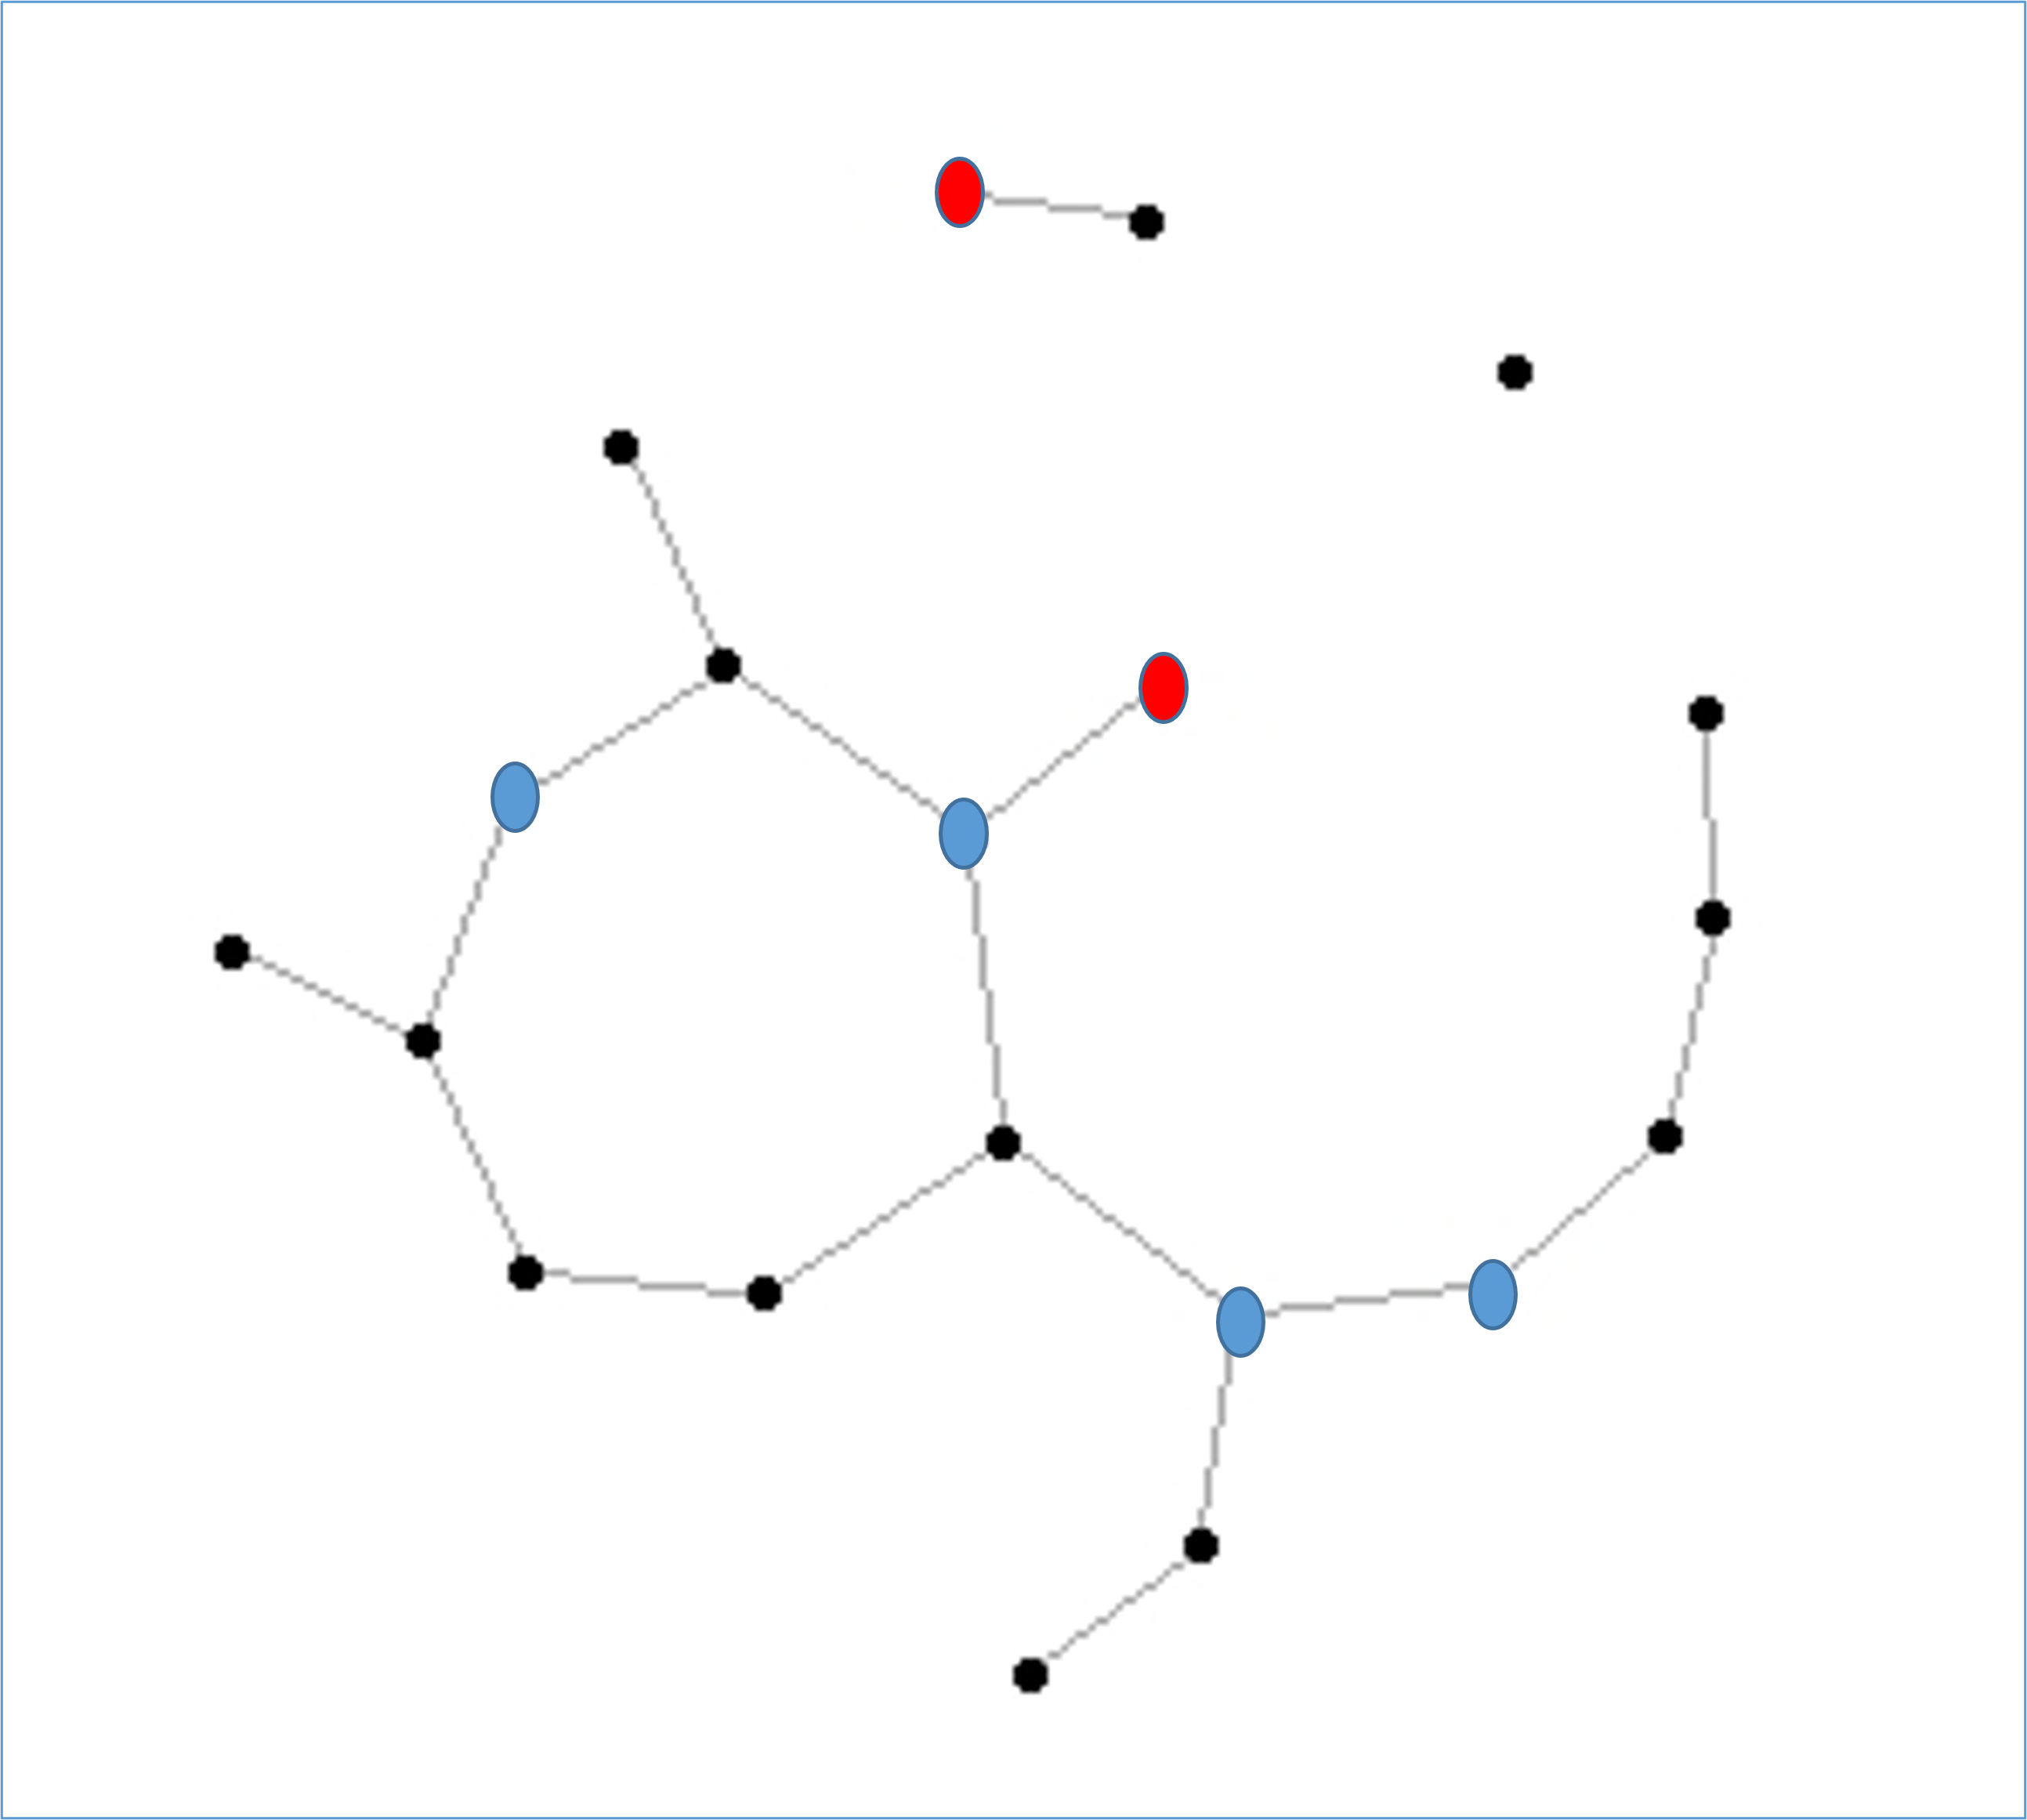
\includegraphics[scale=0.5]{Original Figures/Network Example 5.png}
    \caption{Re-generated network with 20 \% PrEP coverage randomly assigned to uninfected individuals. The 4 blue nodes represent uninfected individuals assigned to PrEP; the 2 red nodes represent individuals living with HIV; the 14 black nodes are individuals without HIV and not assigned to PrEP. }
    \label{fig: Figure 4}
\end{figure}

We can immediately see from a comparison with the previous two figures that the structure of this new network is different. However, it still follows the same basic network parameters as the previous network, with the same number of individuals, the same baseline HIV prevalence, and the same probability of network contacts. There are once again 2 individuals living with HIV and 18 uninfected individuals. Now, 4 uninfected individuals have been assigned to PrEP, only one of whom has an infectious contact. In addition, one other individual not assigned to PrEP has an infectious contact; the remaining 14 uninfected individuals do not have infectious contacts. Now, the counterfactual outcome estimated using Equation \ref{eq:9} will depend on the probability of transmission following an infectious contact while on PrEP and while not on PrEP:

\begin{align}
\begin{split}
E[\hat{Y}\left(\mathbf{\alpha*}|G=g*\right)] & = \frac{\sum_{i=1}^{n}(p_{i})}{N}  \\ 
& = P\left(\hat{Y}|PrEP = 0, Contact = 1\right)P\left(PrEP = 0, Contact = 1\right)  \\ \nonumber
& +P\left(\hat{Y}|PrEP = 0, Contact = 0\right)P\left(PrEP = 0, Contact = 0\right)  \\ \nonumber
& +P\left(\hat{Y}|PrEP = 1, Contact = 1\right)P\left(PrEP = 1, Contact = 1\right) \\ \nonumber
& +P\left(\hat{Y}|PrEP = 1, Contact = 0\right)P\left(PrEP = 1, Contact = 0\right) \\ \nonumber
 &= \frac{1}{18}*p_1 +  \frac{14}{18}*0 +\frac{1}{18}*p_2 +  \frac{3}{18}*0 \\ \nonumber
 &=\frac{p_1+p_2}{18}  \nonumber
 \end{split}
\end{align}

If we were to use this network to estimate the causal effect, without taking the fact that these are network-specific counterfactuals into consideration, we might conclude that this estimates the effect of increasing PrEP coverage from 10\% to 20\%. However, when we consider the quantities that were actually estimated on each network, we notice that this does not estimate either a network-specific effect or an average effect across possible networks unless we can assume that network structure does not affect the counterfactual outcome. That assumption is unreasonable for infectious disease transmission. The estimated counterfactual contrast comparing the single time-step HIV incidence in the two networks, when one has 10\% of eligible individuals treated and the other has 20\% treated, would use the following calculation: 

\begin{equation}\label{eq:12}
E[\hat{Y}\left(\mathbf{\alpha*}|G=g*\right)] -E[Y\left(\mathbf{\alpha}|G=g\right)] = \frac{\left(p_1 +p_2\right)-\left(5p_1\right)}{18}= \frac{p_2-4p_1}{18}.
\end{equation}


Next, consider a scenario where we retain the original network structure from Figures \ref{fig: Figure 2} and \ref{fig: Figure 3} but apply an additional PrEP assignment. There are multiple ways in which we can do this, but for simplicity, we consider the following two options. In the first, we increase PrEP coverage to 20\% by selecting an additional random 10\% of uninfected individuals to receive treatment (additive approach, $\alpha^*$, Figure \ref{fig: Figure 5}). In the second, we discard prior treatment status and choose a random 20\% to receive PrEP (random approach, $\alpha^{**}$ Figure \ref{fig:Figure 6}).


\begin{figure}[H]
    \centering
    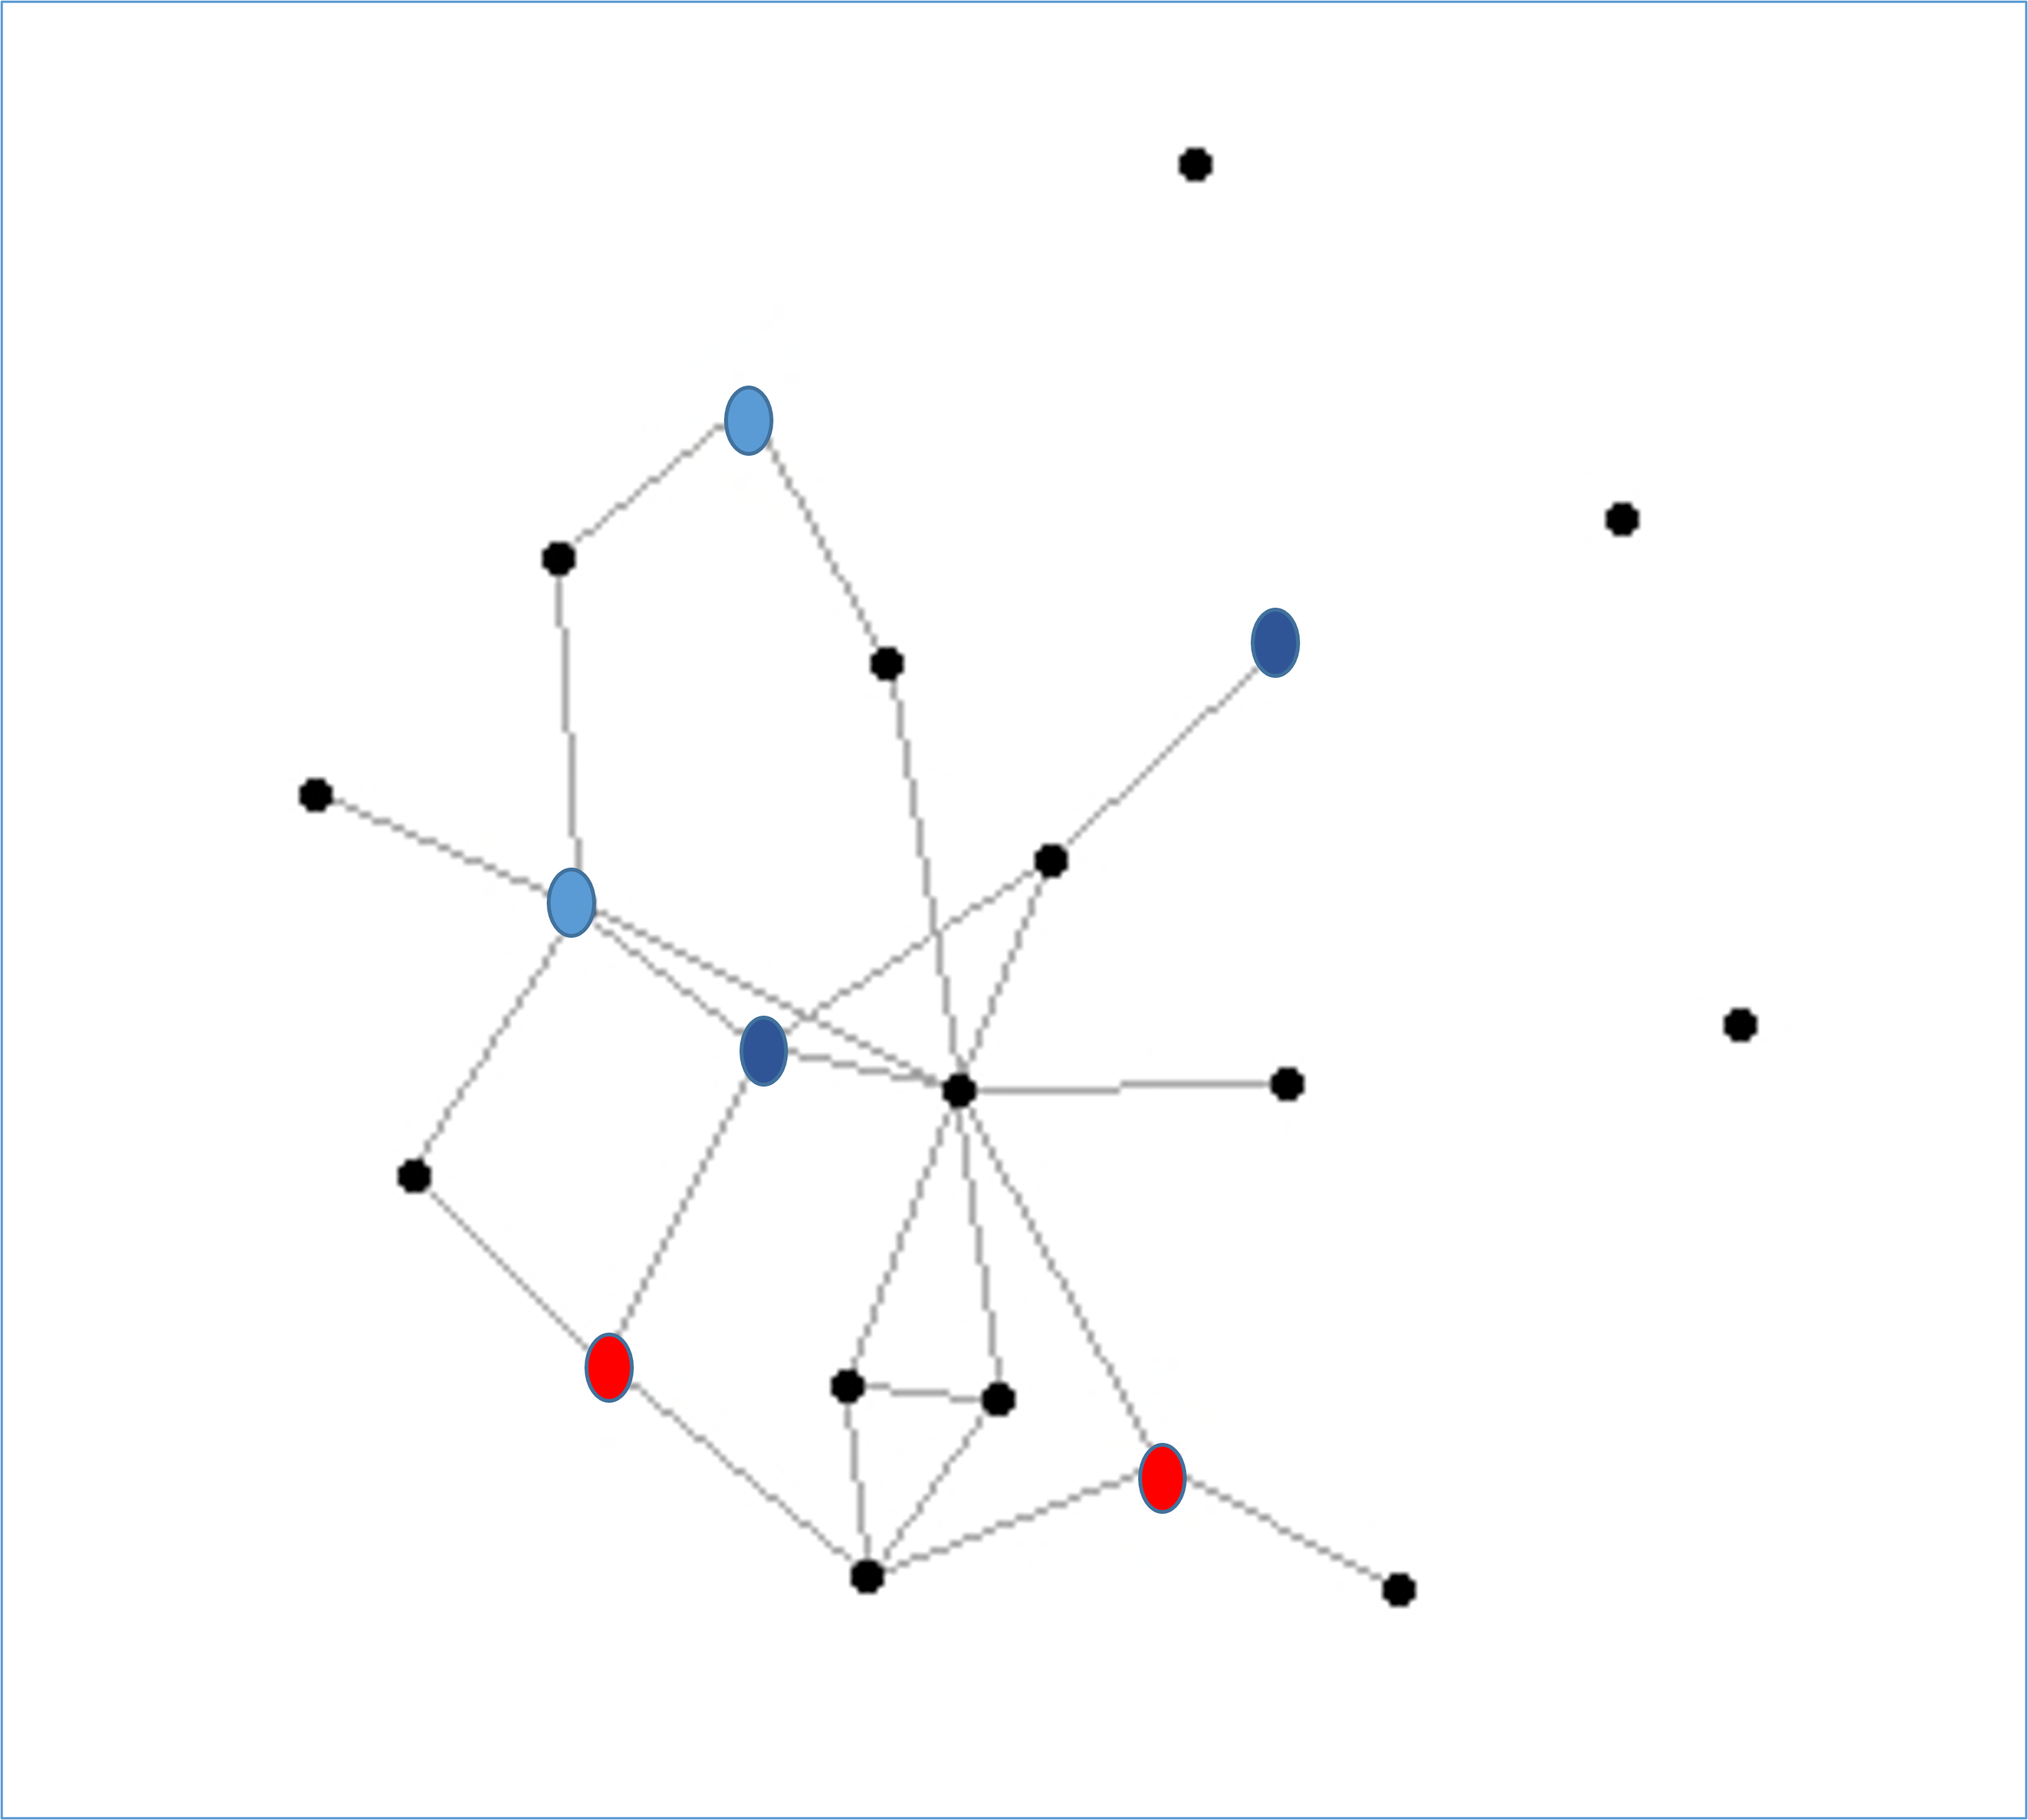
\includegraphics[scale=0.5]{Original Figures/Network Example 4.png}
    \caption{Additive scenario: Network structure from the control scenario, with an additional 10\%  of uninfected individuals randomly assigned to PrEP (treatment strategy $\alpha^*$). Blue nodes represent uninfected individuals assigned to PrEP; red nodes represent individuals living with HIV; black nodes are individuals without HIV and not assigned to PrEP.}
    \label{fig: Figure 5}
\end{figure}

Under the Additive treatment pattern, the original two individuals who were treated but did not have infectious contacts continue to receive treatment. We now additionally provide PrEP to two more randomly selected individuals, of whom one does have an infectious contact. Of the remaining 14 uninfected and untreated individuals, 4 have infectious contacts. We now obtain the following estimate: 

\begin{align}
\begin{split}
E[Y\left(\mathbf{\alpha^*}|G=g\right)] & = \frac{\sum_{i=1}^{n}(p_{i})}{N}  \\ 
& = P\left(Y|PrEP = 0, Contact = 1\right)P\left(PrEP = 0, Contact = 1\right)  \\ \nonumber
& +P\left(Y|PrEP = 0, Contact = 0\right)P\left(PrEP = 0, Contact = 0\right)  \\ \nonumber
& +P\left(Y|PrEP = 1, Contact = 1\right)P\left(PrEP = 1, Contact = 1\right) \\ \nonumber
&  +P\left(Y|PrEP = 1, Contact = 0\right)P\left(PrEP = 1, Contact = 0\right) \\ \nonumber
 &= \frac{4}{18}*p_1 +  \frac{10}{18}*0 +\frac{1}{18}*p_2 +  \frac{3}{18}*0\\ \nonumber
 &=\frac{4p_1+p_2}{18}  \nonumber
 \end{split}
\end{align}

\begin{figure}[H]
    \centering
    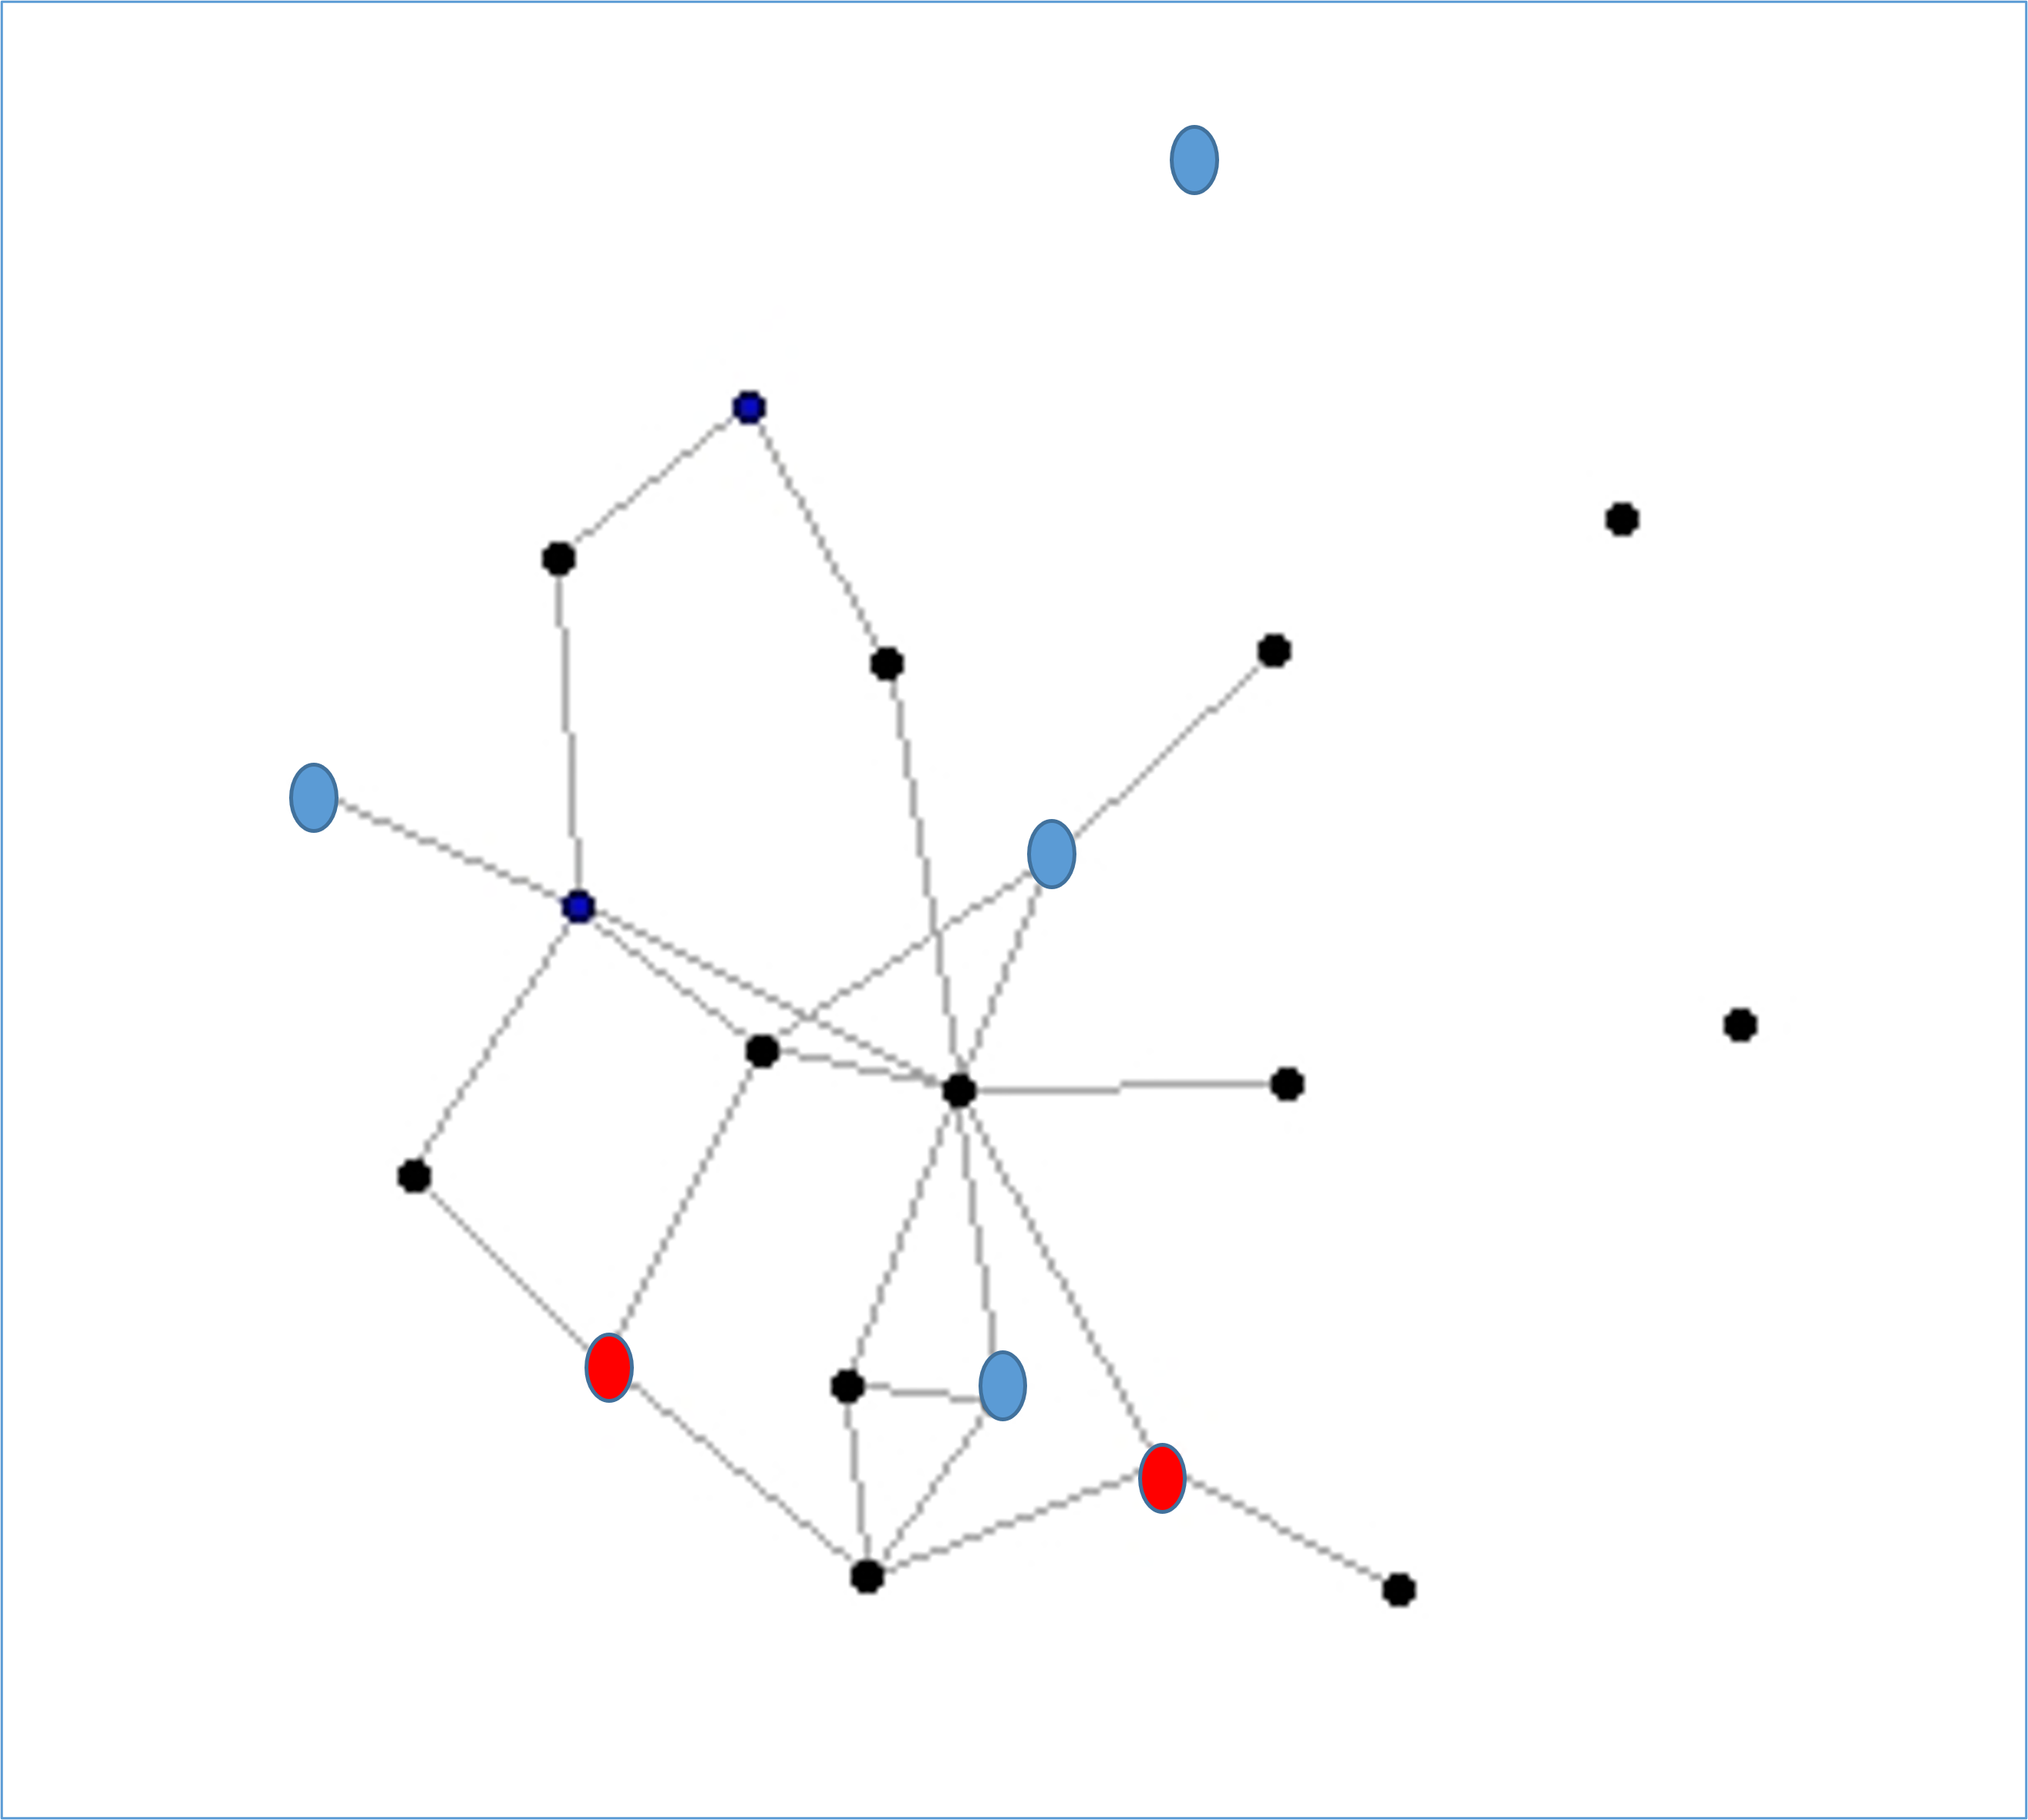
\includegraphics[scale=0.5]{Original Figures/Network Example 3.png}
    \caption{Random scenario: Network structure from the control scenario, with a newly selected 20\%  of uninfected individuals randomly assigned to PrEP  (treatment strategy $\alpha^{**}$). Blue nodes represent uninfected individuals assigned to PrEP; red nodes represent individuals living with HIV; black nodes are individuals without HIV and not assigned to PrEP.}
    \label{fig:Figure 6}
\end{figure}

Under the Random treatment pattern, all four newly selected PrEP recipients do not have an infectious contact. Of the remaining 14 uninfected and untreated individuals, 5 have infectious contacts. This time, we obtain the following estimate: 

\begin{align}\label{eq:14}
\begin{split}
E[Y\left(\mathbf{\alpha^{**}}|G=g\right)] & = \frac{\sum_{i=1}^{n}(p_{i})}{N}  \\ 
& = P\left(Y|PrEP = 0, Contact = 1\right)P\left(PrEP = 0, Contact = 1\right)  \\ \nonumber
& +P\left(Y|PrEP = 0, Contact = 0\right)P\left(PrEP = 0, Contact = 0\right)  \\ \nonumber
& +P\left(Y|PrEP = 1, Contact = 1\right)P\left(PrEP = 1, Contact = 1\right) \\ \nonumber
&  +P\left(Y|PrEP = 1, Contact = 0\right)P\left(PrEP = 1, Contact = 0\right) \\ \nonumber
 &= \frac{5}{18}*p_1 +  \frac{10}{18}*0+\frac{0}{18}*p_2 +  \frac{4}{18}*0  \\ \nonumber
 &=\frac{5p_1}{18}  \nonumber
 \end{split}
\end{align}

Comparing these results to our initial 10\% PrEP coverage scenario, we obtain the following estimates. For the Additive treatment pattern, we get:

\begin{equation}\label{eq:15}
E\left[Y\left(\mathbf{\alpha*}-\mathbf{\alpha}|G=g\right)\right] =  E[Y\left(\mathbf{\alpha^*}|G=g\right) -Y\left(\mathbf{\alpha}|G=g\right) = 
\frac{\left(4p_1+p_2\right)-\left(5p_1\right)}{18}=
\frac{p_2-p_1}{18}
\end{equation}

and for the Random treatment pattern, we get:
\begin{equation}\label{eq:16}
E\left[Y\left(\mathbf{\alpha^{**}}-\mathbf{\alpha}|G=g\right)\right] =E[Y\left(\mathbf{\alpha^{**}}|G=g\right) -Y\left(\mathbf{\alpha}|G=g\right)] = \frac{5p_1}{18} - \frac{5p_1}{18} =0.
\end{equation}

Note that like with the regenerated network scenario, all quantities in these contrasts are network-specific counterfactuals. However, unlike with the regenerated network, the new 20\% treatment counterfactuals are estimated conditional on the same network as the reference scenario counterfactuals. This provides a valid estimate of network-specific effects, even if these effects are not generalizable to all possible networks of this type. Also, note that causal effects estimated by equations \ref{eq:15} and \ref{eq:16} differ because they involve different treatment pattern comparisons.


\section{Amount of bias depends on network features}
In the previous section, we compared only two counterfactual estimates. More realistically, counterfactuals would be simulated multiple times each, so that the average effect could be estimated rather than the network-specific effect. As shown, the network-specific effect should be estimated by comparing network-specific counterfactuals before pooling across network realizations. However, this is only true because we cannot typically simulate all possible network realizations. We might expect that as the number of realizations simulated increases to infinity, the potential bias from using the regeneration approach should reduce to zero, at least when using a difference-based estimator.

Another important determinant of the expected bias is the size of the two parameters $n$ (individuals with infectious contacts) and $k$ (individuals receiving PrEP) relative to the size of the uninfected population $N$. If we randomly generate networks from our distribution and randomly assign treatment to uninfected individuals, there are $\binom{N}{k}$ unique network realizations where $k$ individuals are treated. 

In each realization, some portion $n \le N$ will have an infectious contact. We can separate all possible network realizations into those in which at least one individual is both treated and has an infectious contact, and those in which all treated individuals have no infectious contact. Only for network realizations of the first type will treatment have any effect on the outcome -- when all treated individuals have no infectious contacts, there is no benefit to treatment in that time step. We call network realizations with at least one treated individual with infectious contact informative networks. The probability, $P$, of an informative network for a network of size $N$, with $n$ individuals with infectious contacts and $k$ treated individuals is (see Appendix \ref{Appendix 1} for derivation):

\begin{equation}\label{eq:17}
    \frac{{\binom{N}{k}}-{\binom{N-n}{k}}}{{\binom{N}{k}}}=1-\left(1-\frac{k}{N}\right)^{n}
\end{equation}

That is, the probability, $P$, of at least one node $i$ assigned to treatment with at least one infectious contact for a given network structure $g$ and treatment assignment is:
\begin{equation}\label{eq:18}
    P \coloneqq \mathbb{P}\left(n_{i}=1 \vert k_{i}=1,j,\alpha,\alpha*\right)=1-\left(1-\frac{k}{N}\right)^{n}
\end{equation}
When $P$ is large, the majority of network realizations can be expected to contribute at least some information to the average effect. However, when $P$ is small, we can expect that most network realizations will be uninformative -- that is, most realizations of the network will be ones in which no individual is both treated and exposed to an infectious contact. Therefore, the magnitude of $P$ can provide insight into the number of realizations we need to simulate to obtain a stable estimate of effects across all network structures. In addition, note that
\begin{equation}\label{eq:19}
    \lim_{N \to \infty}P=\begin{cases}0 & k,n \text{ fixed} \\ 1 & k \to N \lor n \to N  \end{cases}
\end{equation}

That is, as the size of the uninfected network population increases, $P$ is expected to approach 0 for a fixed number of individuals receiving treatment and a fixed number with infectious contact. On the other hand, if either the number of individuals treated or the number of individuals with infectious contact approaches the total number of uninfected individuals, then as $N$ increases, the value of $P$ will approach 1.

\section{Simulation example}
To demonstrate the potential impact of the simulation approach, we repeated our simplified example across multiple network realizations. In the following section, we describe the simulation methods and results of this process.

 \subsection{Methods}
We considered three types of network-based simulation models. Network models were parameterized according to network size (graph order), and the generative model specifying the probability distribution from which the graph was drawn or the algorithm used to construct the graph. Let $deg(v)$ denote the degree, or the number of immediate connections, of node $v$.

We first implemented the  Erdős–Rényi (ER) Random Graph Model with $G(N,p)$ parameterization \cite{barabasi_network_2016}, scaling the edge formation probability by the network size such that $p \coloneqq \frac{3}{N}$. This was done to avoid networks with full connectivity in which every individual is connected to every other individual. In this latter case, all possible network realizations will be informative since if every individual has a direct edge to every other individual then all treated individuals will necessarily have an edge connection to all infectious individuals thus the maximum direct benefit of treatment will be observed. 
% under which each of $N$ nodes has a binomially-distributed degree:
% \begin{equation*}
  %  \mathbb{P}(deg(v)=k)=\binom{n-1}{k}p^{k}\left(1-p\right)^{n-1-k}, \quad \forall v \in V . 
% \end{equation*}

We also implemented two other network generative models to assess the importance of specific aspects of network structure: \textit{preferential attachment} and \textit{clustering}. 

To assess preferential attachment, we implemented a Barabási–Albert (BA) scale-free graph model\cite{barabasi_network_2016}. This model involved constructing an initial connected graph, then adding a new node connected to the existing node $i$ with probability 
\begin{equation*}
    p_{i}=\frac{k_{i}}{\sum_{j}k_{j}}.
\end{equation*}

We use a generalization of the BA model, sometimes called the Nonlinear Preferential Attachment Model, with power parameter $\alpha$, where the degree distribution is given by:
\begin{equation*}
    p_{i}=\frac{k_{i}^{\alpha}}{\sum_{j}k_{j}^{\alpha}}.
\end{equation*}

Finally, to assess clustering, we used a Watts-Strogatz (WS) small-world network model \cite{watts_collective_1998}. The construction algorithm relied on 4 parameters: the dimension of the initial lattice, here always equal to 1 since the standard WS model begins with a one-dimensional ring lattice \cite{barrat_properties_2000}, the size of the graph in each dimension (here always the final graph order $N$), the connected \textit{neighborhood size} $n$, and the rewiring probability $r$. The initial graph is a lattice where each node is connected to its $n$ neighbors. From the initial lattice graph, edges are randomly ``rewired", i.e., removed and connected to a different node, uniformly with probability $r$.

For each model type, we simulated the counterfactual infection probability after one time step when 20\% of uninfected individuals were prescribed PrEP at random. We assume that treatment is assigned randomly to all eligible (uninfected) individuals, with no attempt to target treatment based on an individual's outcome risk. Completely random treatment is unrealistic in most real-world settings. However, even when good data are collected, we generally do not know with certainty for every single individual whether or not they have an infectious contact at the time of treatment. In addition, we focus on a single time step to avoid consideration of time-varying network structure changes.

In addition, we simulated comparison counterfactual data under 40\% of uninfected individuals prescribed PrEP, using the three approaches described in the previous simplified example: (1) Additive approach -- 40\% coverage is achieved by adding an additional 20\% coverage to the existing 20\% coverage on a given network realization; (2) Random approach -- 40\% and 20\% coverage estimates obtained from random treatment on a given network realization; and (3) Regenerated approach -- 40\% and 20\% coverage estimates obtained from random treatment on different network realizations. We used each approach to estimate the average overall effect of 40\% versus 20\% PrEP coverage across a range of network model parameters (Table \ref{tab:table1}).

\newpage
%%NOTE: please combine the two tables below with a column indicating which model type(s) the parameter applies to. Also, I'm not sure how to do the table caption, so please correct that. Thanks!
\begin{landscape}
\begin{table}[H]
    \centering
    \begin{tabular}{|c|c|c|c|c|}
    \hline
    \bf Parameter & \bf Model & \bf Alias in Code & \bf Default Value & \bf Range Considered  \\
    \hline
    Network size & Erdős–Rényi& $N$& 20 & $\Set{20,200}$\\
    \hline
    Network size & Watts-Strogatz and Barabási–Albert & $N$& 50 & Fixed \\
    \hline
    ER Edge Formation probability & Erdős–Rényi & ``eprob" & $\frac{3}{N}$ & Fixed \\
    \hline
    HIV prevalence & All & ``phiv" & 0.1 & $[0.1,0.8]$\\
    \hline
    Control PrEP Coverage & All & ``PrEP1" & 0.2 & $[0.1,1]$\\
    \hline
    Counterfactual PrEP Coverage & All & ``PrEP2" & 0.4 & $[0.1,1]$\\
    \hline
    $\mathbb{P}\left[\text{HIV} \vert \neg \text{PrEP} \cap \text{Contact}\right]$ & All & ``p1" & 0.2 & $[0.1,1]$\\
    \hline
    $\mathbb{P}\left[\text{HIV} \vert \text{PrEP} \cap \text{Contact}\right]$ & All & ``p2"  & 0.1 & $[0.1,1]$\\
    \hline
    Number of network realizations & All & ``nsim" & 200 & $\Set{200,2000,20000}$\\
    \hline
    Preferential Attachment power & Barabási–Albert& ``pow" & 1 & $\left[1,2 \right]$ \\
    \hline
    Neighborhood size & Watts-Strogatz & ``nb" & 5 & $\Set{5,10,15,20}$ \\
    \hline
    Rewiring probability & Watts-Strogatz &  ``rprob" & 0.05 &$\left[0.05, 0.95 \right]$ \\
    \hline
    \end{tabular}
    \caption{Parameters used in Static Network Simulation models. Abbreviations: ER = Erdős–Rényi; PrEP = pre-exposure prophylaxis; HIV = human immunodeficiency virus.}
    \label{tab:table1}
\end{table}
\end{landscape}
\newpage


Simulations were implemented in R 4.2.1. All code, data, and figure files are available in the GitHub repository: \href{https://github.com/nico-dangelo/Network-Spillover}{Network Spillover}\footnote{https://github.com/nico-dangelo/Network-Spillover}. Network graphs were generated using igraph version 1.3.2. \cite{csardi_igraph_2005}. 
%Parallel implementation used the package ‘furrr’ version 0.3.0 \cite{vaughan_furrr_2022}


\section{Results}


Across all simulation parameter sets and model types, we see that the general patterns in the risk difference estimates match our expectations. We anticipated biased results from the regeneration approach. We also anticipated that the additive and random approaches would have less bias but return different results from each other due to the different causal questions assessed. In general, this is what we found in our simulation. When the Additive or Random approaches are used, there is a smaller variance in the average risk difference estimates across runs, and a more predictable pattern of mean risk difference estimates across input parameters. By contrast, when the Regenerated approach is used, the variance of the risk difference estimates is typically larger and more variable across the parameter input space, and the patterns in mean risk difference estimates are inconsistent across parameter inputs. We highlight several representative results next and include the results of all parameter variations in the Supplementary Appendix (\ref{Appendix 4}).

\subsection{Network size and number of network realizations}
As predicted by our combinatorics result, for a fixed probability of infectious contacts and a fixed proportion treated in the two treatment conditions (40\% treated versus 20\% treated), the mean risk difference gives a more variable estimate of the average overall treatment effect when the network size is smaller, and this variability is larger when using the Regenerated approach. Figure \ref{fig:Figure 7} shows the pattern of risk difference estimates in one time-step across values of the probability of HIV infection for individuals with an infectious contact, when receiving PrEP (y-axis) versus when not receiving PrEP (x-axis). Individuals with infectious contact are the only individuals in the model who can acquire HIV infection in a single time-step. For each subgraph, the diagonal line from the bottom left corner to the upper right corner (i.e., the line $y=x$) represents the scenario where the probability of infection is the same regardless of PrEP status. For these squares, the true average overall effect across all possible network realizations should be the null (i.e., 0). The area above this diagonal represents scenarios where HIV infection is \textit{more} common when taking PrEP, and thus, we expect the true overall effect to be greater than 0; the area below the diagonal represents scenarios where HIV infection is less common when taking PrEP and the true effect should be below 0. 

The results obtained using the Regenerated contrast are in conflict with our expected true patterns of effects when the network is small (Figure \ref{fig:Figure 7}). The Additive and Random approaches correctly recover the effect patterns we expect regardless of network size (see Supplementary Appendix \ref{Appendix 4} for variance plots). 


\begin{figure}[H]
    \centering
    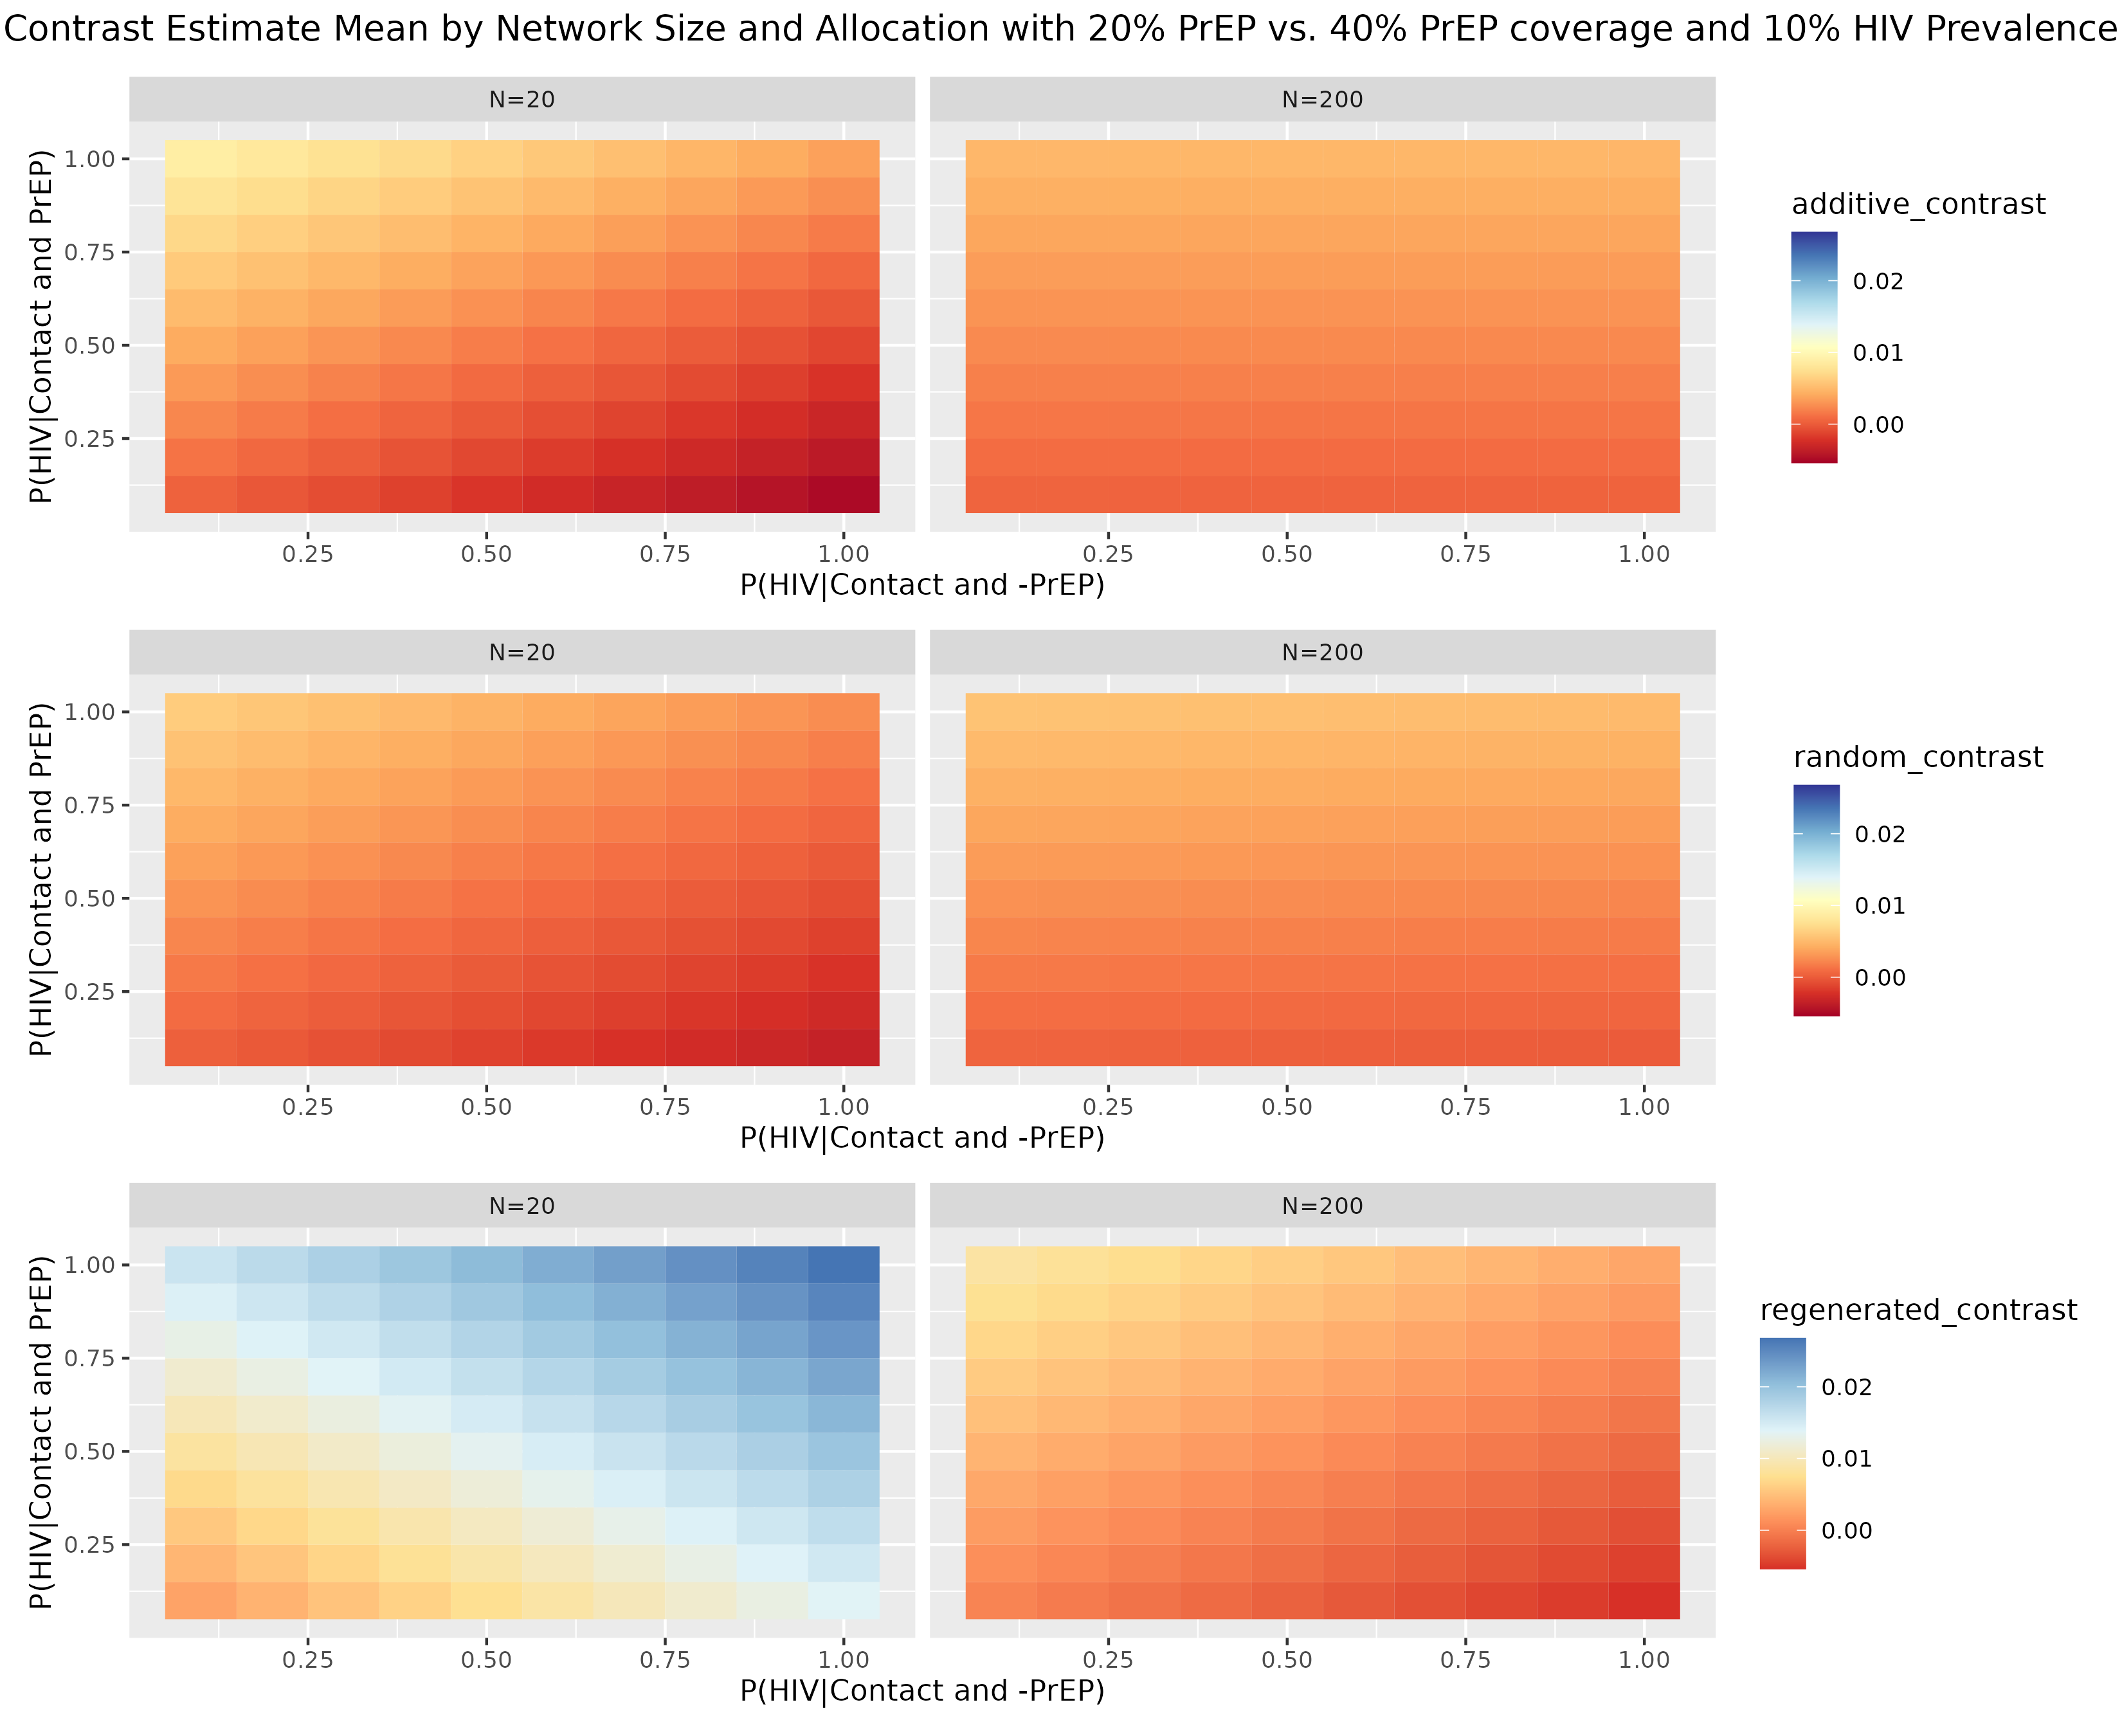
\includegraphics[width=\linewidth]{Corrected Figures/Network Size Mean Plot.png}
    \caption{Mean risk difference estimates comparing number of new infections when 40\% versus 20\% of uninfected nodes are treated with PrEP across varying levels of $\mathbb{P}\left[\text{HIV} \vert \neg \text{PrEP} \cap \text{Contact}\right]$ and $\mathbb{P}\left[\text{HIV} \vert \text{PrEP} \cap \text{Contact}\right]$, stratified by Network Size and using 200 simulation samples 
    From top to bottom: ``Additive" approach increases the proportion on PrEP compared to a given network realization and given set of treated nodes; ``Random" approach compares PrEP allocation levels for a given network realization, without fixing the treated nodes; ``Regenerated" approach compares PrEP levels without fixing network realization or treated nodes. }
    \label{fig:Figure 7}
\end{figure}

We see a similar set of patterns when we hold the network size fixed but vary the number of realizations simulated. The difference between the approaches here is most clearly visualized by a plot of the variance in risk difference estimate across all runs (Figure \ref{fig:Figure 8}). The variance in the risk difference estimates is smallest for the Additive approach and largest for the Regenerated approach. 

\begin{figure}[H]
    \centering
    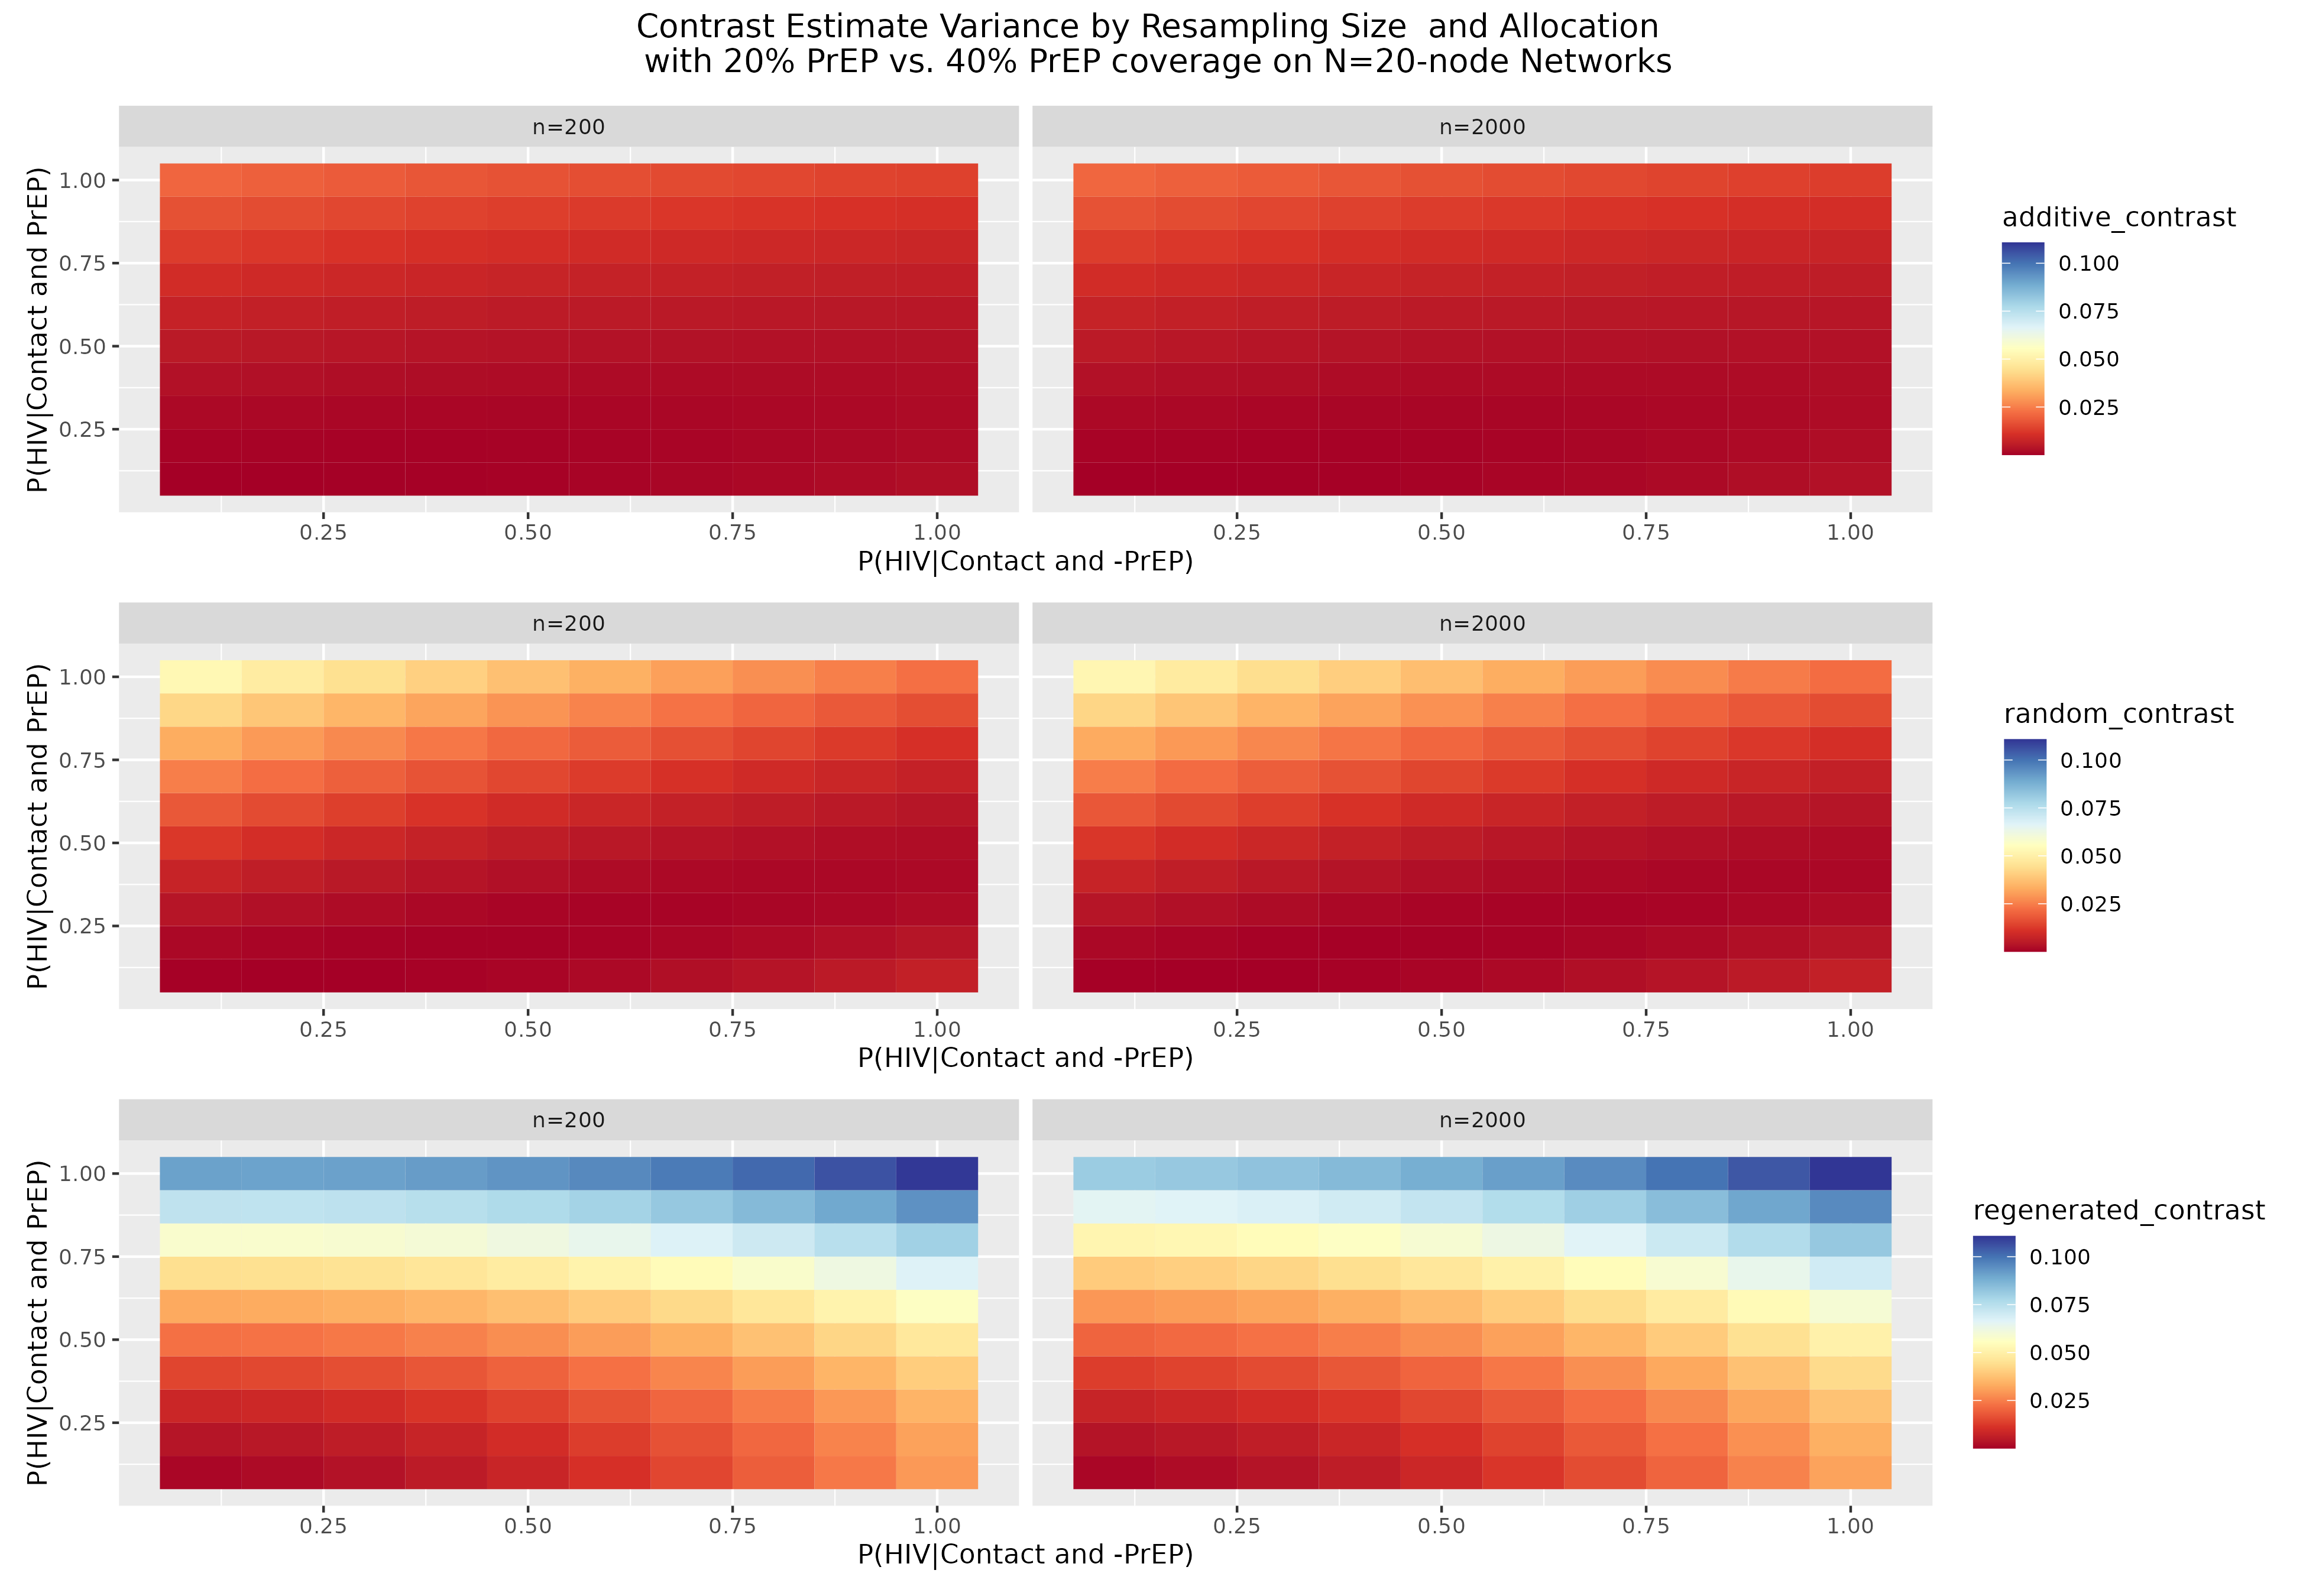
\includegraphics[width=\linewidth]{Corrected Figures/Resampling Size Variance Plot.png}
    \caption{Variance of risk difference estimates comparing number of new infections when 40\% versus 20\% of uninfected nodes are treated with PrEP across varying levels of $\mathbb{P}\left[\text{HIV} \vert \neg \text{PrEP} \cap \text{Contact}\right]$ and $\mathbb{P}\left[\text{HIV} \vert \text{PrEP} \cap \text{Contact}\right]$, stratified by number of simulations sampled when network size is 20 %%PLEASE ADD%%. 
    From top to bottom: ``Additive" approach increases the proportion on PrEP compared to a given network realization and given set of treated nodes; ``Random" approach compares PrEP allocation levels for a given network realization, without fixing the treated nodes; ``Regenerated" approach compares PrEP levels without fixing network realization or treated nodes. }
    \label{fig:Figure 8}
\end{figure}

\subsubsection{Probabilities of infectious contact and infection given contact}
As described above, we anticipate that as either the proportion of individuals with an infectious contact or the proportion treated increases to the size of the uninfected network nodes, the proportion of network realizations in which at least one node has both treatment and an infectious contact will increase towards 100\%. However, at higher values of treatment and/or infectious contact, we might also expect to see greater variation in the \textit{number} of nodes with both treatment and infectious contact across network realizations. Comparing the estimated risk difference across increasing HIV infection prevalence (and thus increasing the probability that any uninfected individual has an infectious contact), we see that the variance is smallest and relatively constant when using the Additive approach but larger and more variable when using the Regenerated approach (Figure \ref{fig:Figure 9}).


\begin{figure}[H]
    \centering
    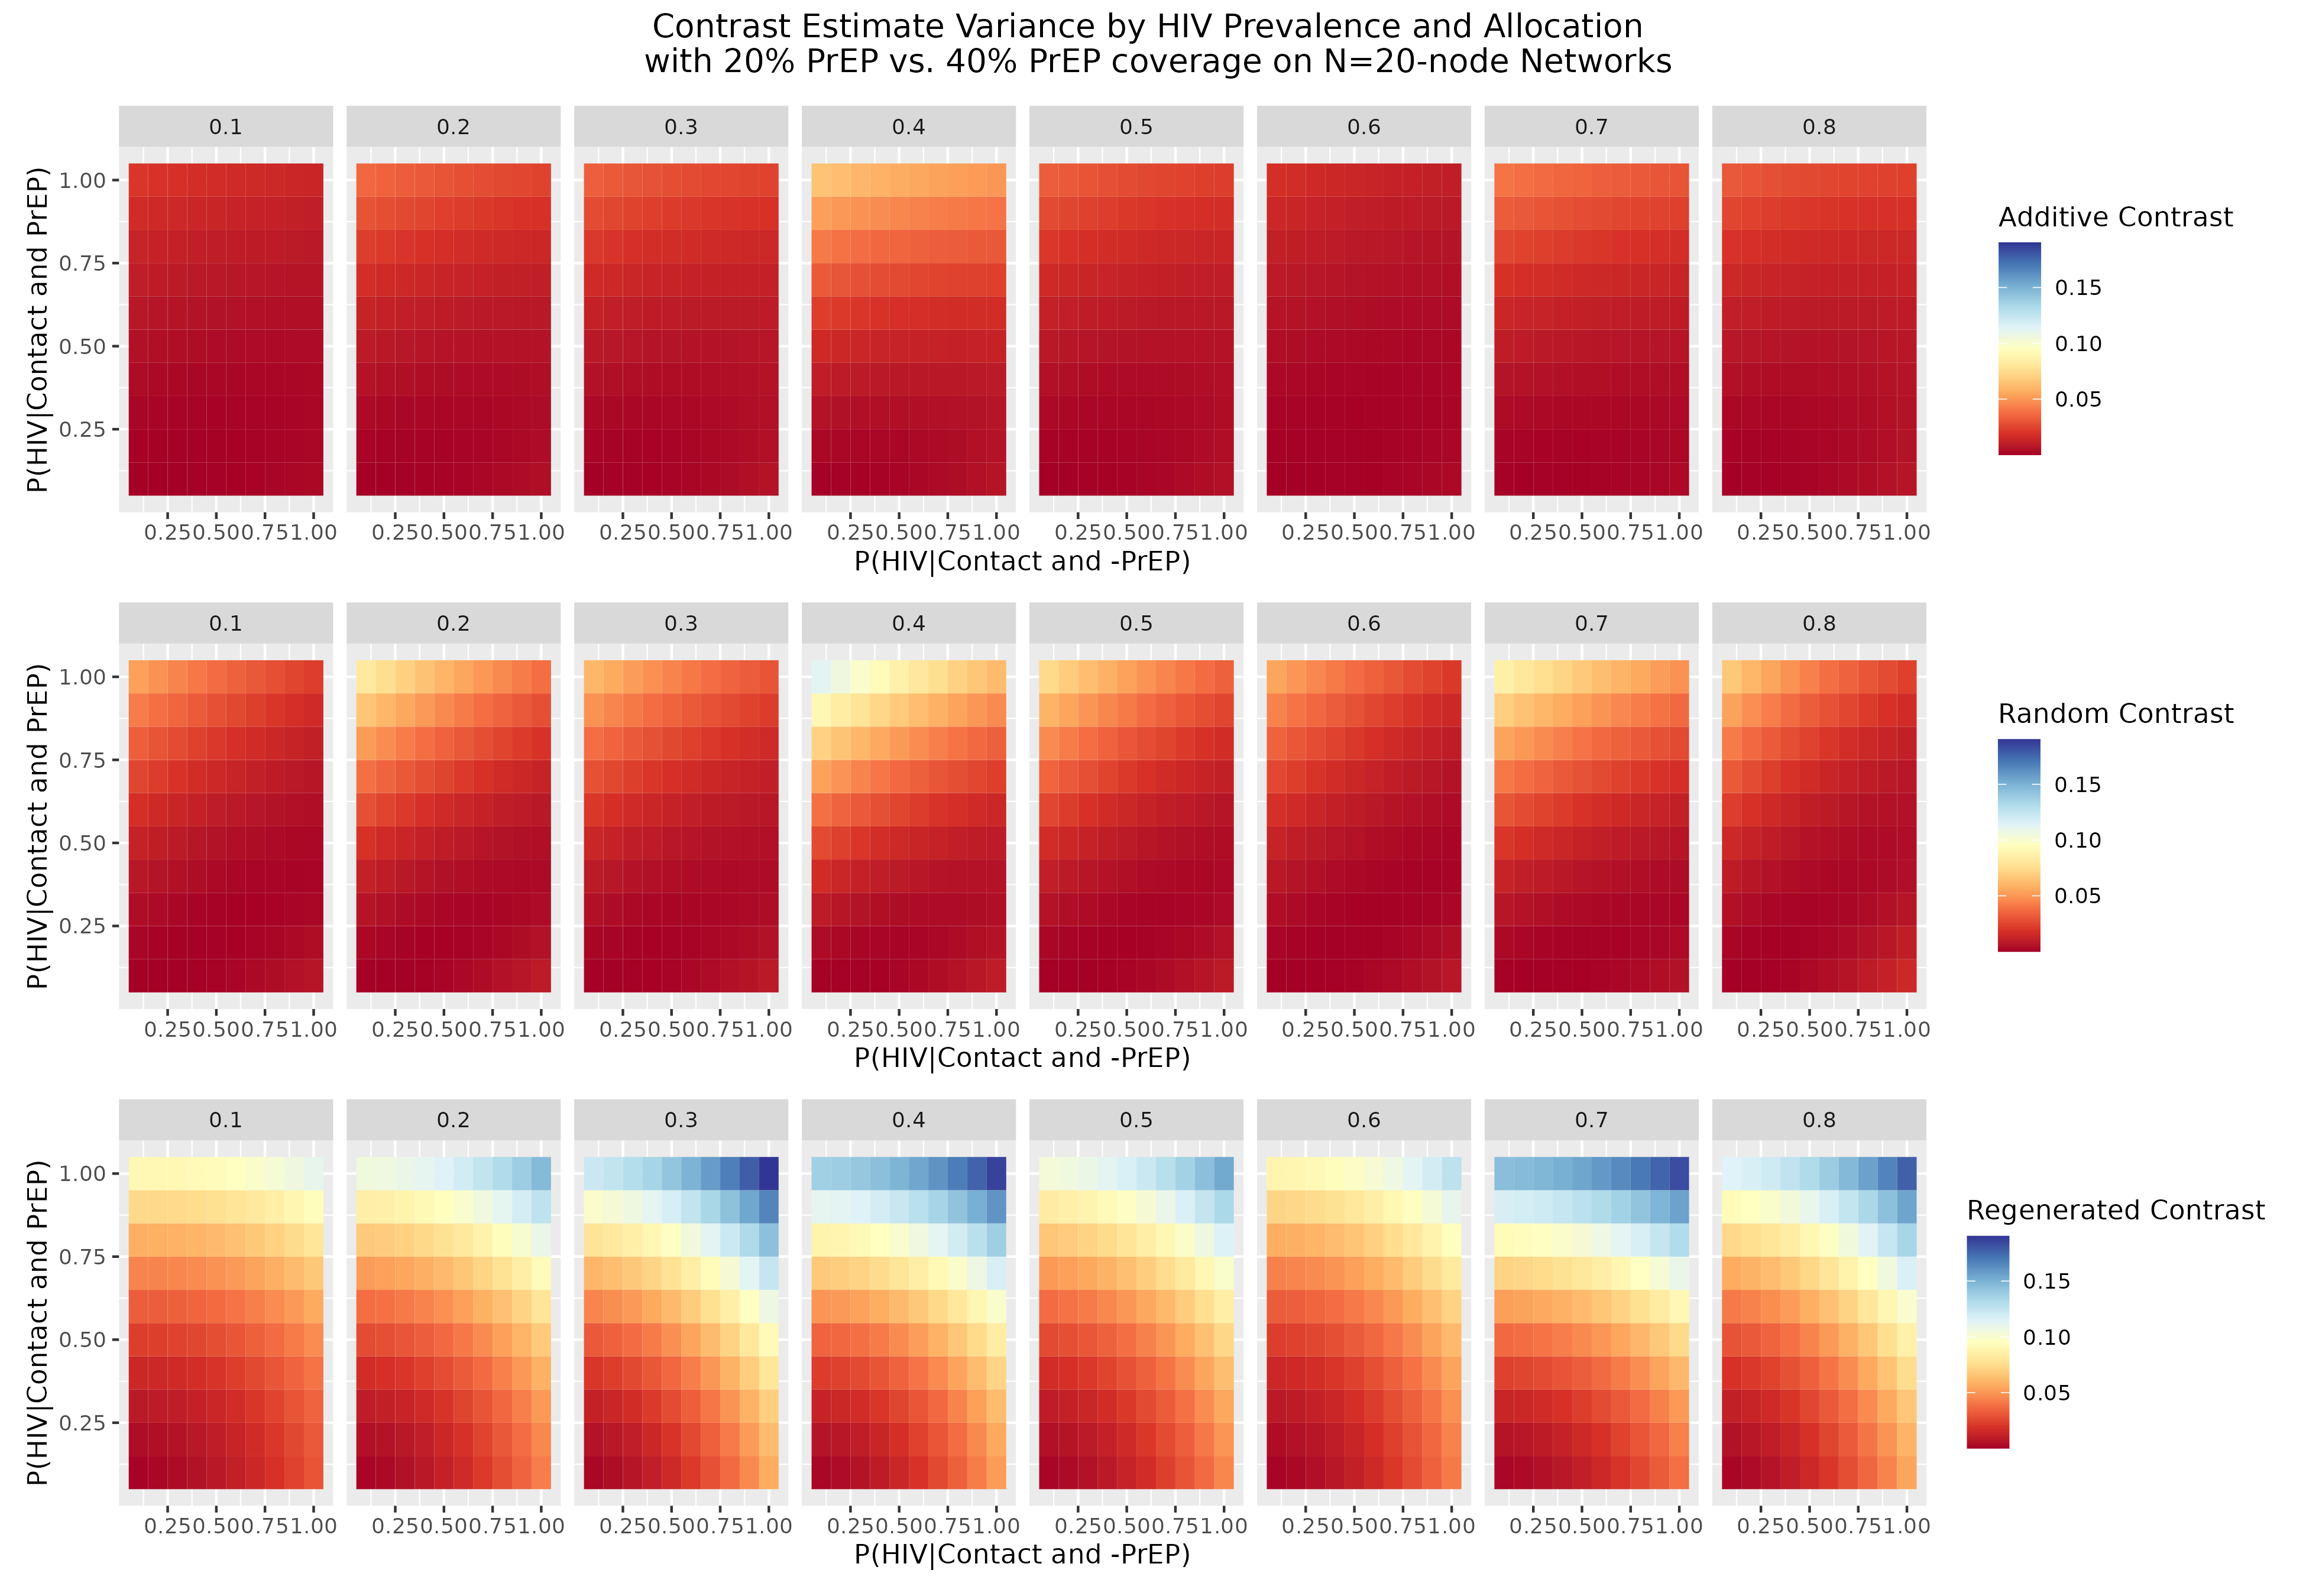
\includegraphics[width=\linewidth]{Corrected Figures/HIV Prevalence Variance Plot.png}
    \caption{Variance of risk difference estimates comparing number of new infections when 40\% versus 20\% of uninfected nodes are treated with PrEP across varying levels of $\mathbb{P}\left[\text{HIV} \vert \neg \text{PrEP} \cap \text{Contact}\right]$ and $\mathbb{P}\left[\text{HIV} \vert \text{PrEP} \cap \text{Contact}\right]$, stratified by starting HIV prevalence in the network with network size of 20 and 200 simulation samples.
    From top to bottom: ``Additive" approach increases the proportion on PrEP compared to a given network realization and given set of treated nodes; ``Random" approach compares PrEP allocation levels for a given network realization, without fixing the treated nodes; ``Regenerated" approach compares PrEP levels without fixing network realization or treated nodes.}
    \label{fig:Figure 9}
\end{figure}


When we hold the probability of infection given either no PrEP (Figure \ref{fig:Figure 10}) or PrEP (Figure \ref{fig:Figure 11}) constant and vary the other, we see that the patterns in estimated mean risk difference are similar for the Additive and Random approaches but very different for the Regenerated approach. As expected, as the probability of HIV infection for individuals with infectious contacts but no PrEP increases, the risk differences for infection with 20\% PrEP coverage compared to 40\% coverage becomes more negative indicating an increasing benefit of having higher PrEP coverage when using the Additive or Random approaches (Figure \ref{fig:Figure 10}). That is, as the risk to the untreated increases, the total number of new infections decreases as more at-risk individuals are treated. For these two approaches, we also see the expected pattern when we simulate an ineffective version of PrEP such that the probability of HIV infection for individuals with both infectious contacts and PrEP increases. When the probability of infection with PrEP exceeds the probability of infection without PrEP the result of increased coverage should be more infections. Indeed, as the probability of infection on PrEP increases, the risk difference approaches the null and becomes positive, indicating an increasingly harmful effect of higher coverage levels (Figure \ref{fig:Figure 11}). In contrast, the Regenerated approach returns the same risk difference pattern regardless of whether the altered probability is that of infection with PrEP or without PrEP.


\begin{figure}[H]
    \centering
    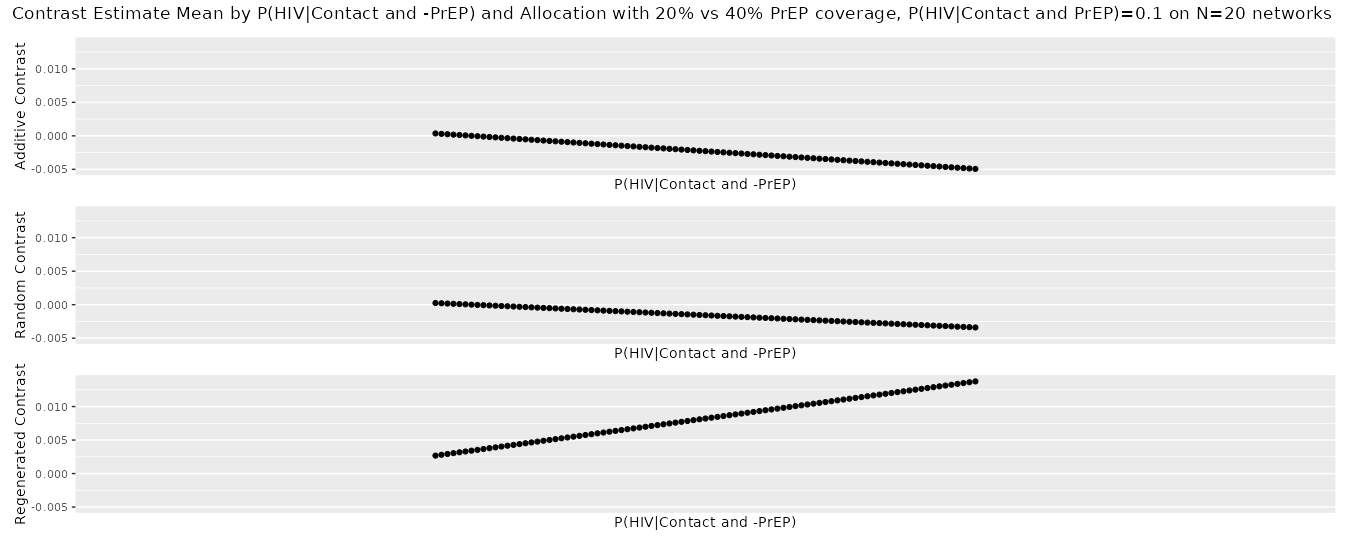
\includegraphics[width=\linewidth]{Corrected Figures/p1 Mean plots.png}
    \caption{Mean risk difference estimates comparing the number of new infections when 40\% versus 20\% of uninfected nodes are treated with PrEP across varying levels of  $\mathbb{P}\left[\text{HIV } \vert \text {Contact } \cap \neg \text{ PrEP}\right]$, with network size of 20,  200 simulation samples,  10\% HIV prevalence at baseline, and a 10 \% probability of infection given contact and PrEP.
    From top to bottom: ``Additive" approach increases the proportion on PrEP compared to a given network realization and given set of treated nodes; ``Random" approach compares PrEP allocation levels for a given network realization, without fixing the treated nodes; ``Regenerated" approach compares PrEP levels without fixing network realization or treated nodes.}
    \label{fig:Figure 10}
\end{figure}

\begin{figure}[H]
    \centering
    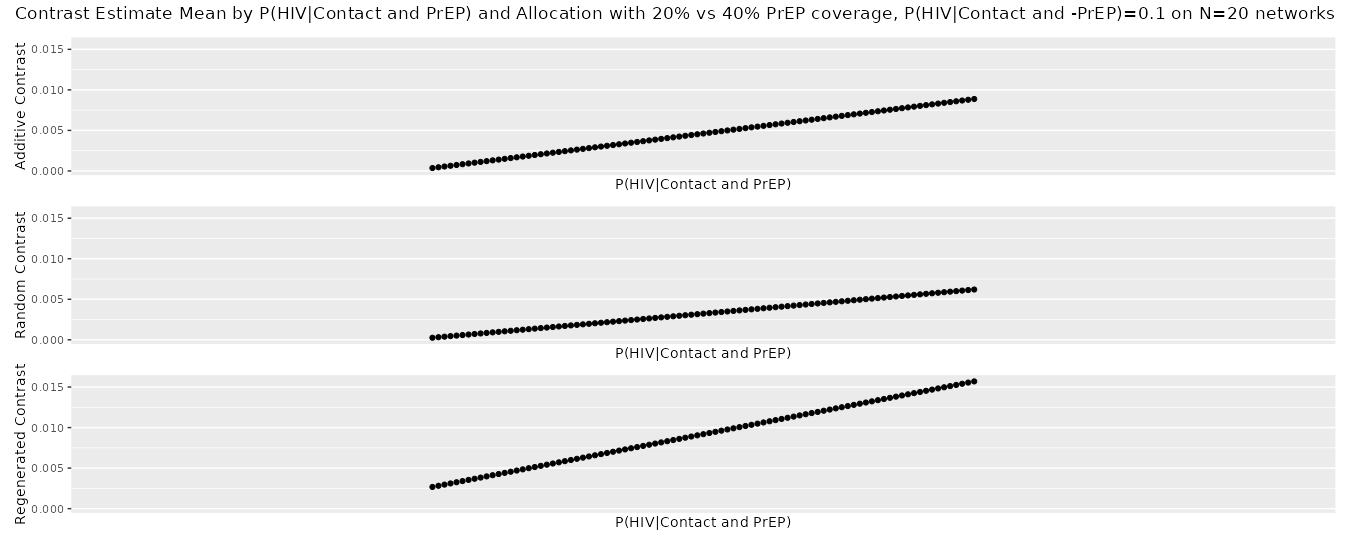
\includegraphics[width=\linewidth]{Corrected Figures/p2 Mean plots.png}
    \caption{
    Mean risk difference estimates comparing the number of new infections when 40\% versus 20\% of uninfected nodes are treated with PrEP across varying levels of  $\mathbb{P}\left[\text{HIV } \vert \text{ PrEP}\right]$, with network size of 20,  200 simulation samples,  10\% HIV prevalence at baseline, and a 10 \% probability of infection given contact and no PrEP.
     From top to bottom: ``Additive" approach increases the proportion on PrEP compared to a given network realization and given set of treated nodes; ``Random" approach compares PrEP allocation levels for a given network realization, without fixing the treated nodes; ``Regenerated" approach compares PrEP levels without fixing network realization or treated nodes.}
    \label{fig:Figure 11}

\end{figure}

\subsubsection{Network model type}
The patterns observed with the Erdos-Renyi network graphs were even more pronounced using the Barabasi-Albert scale-free model  but less so with the Watts-Strogatz Small-world model (Figure \ref{fig:Figure 12}). Likely, this is because of less variation in allowed contact patterns between WS network realizations, given the requirement of a fully-connected graph. 


\begin{figure}[H]
    \centering
    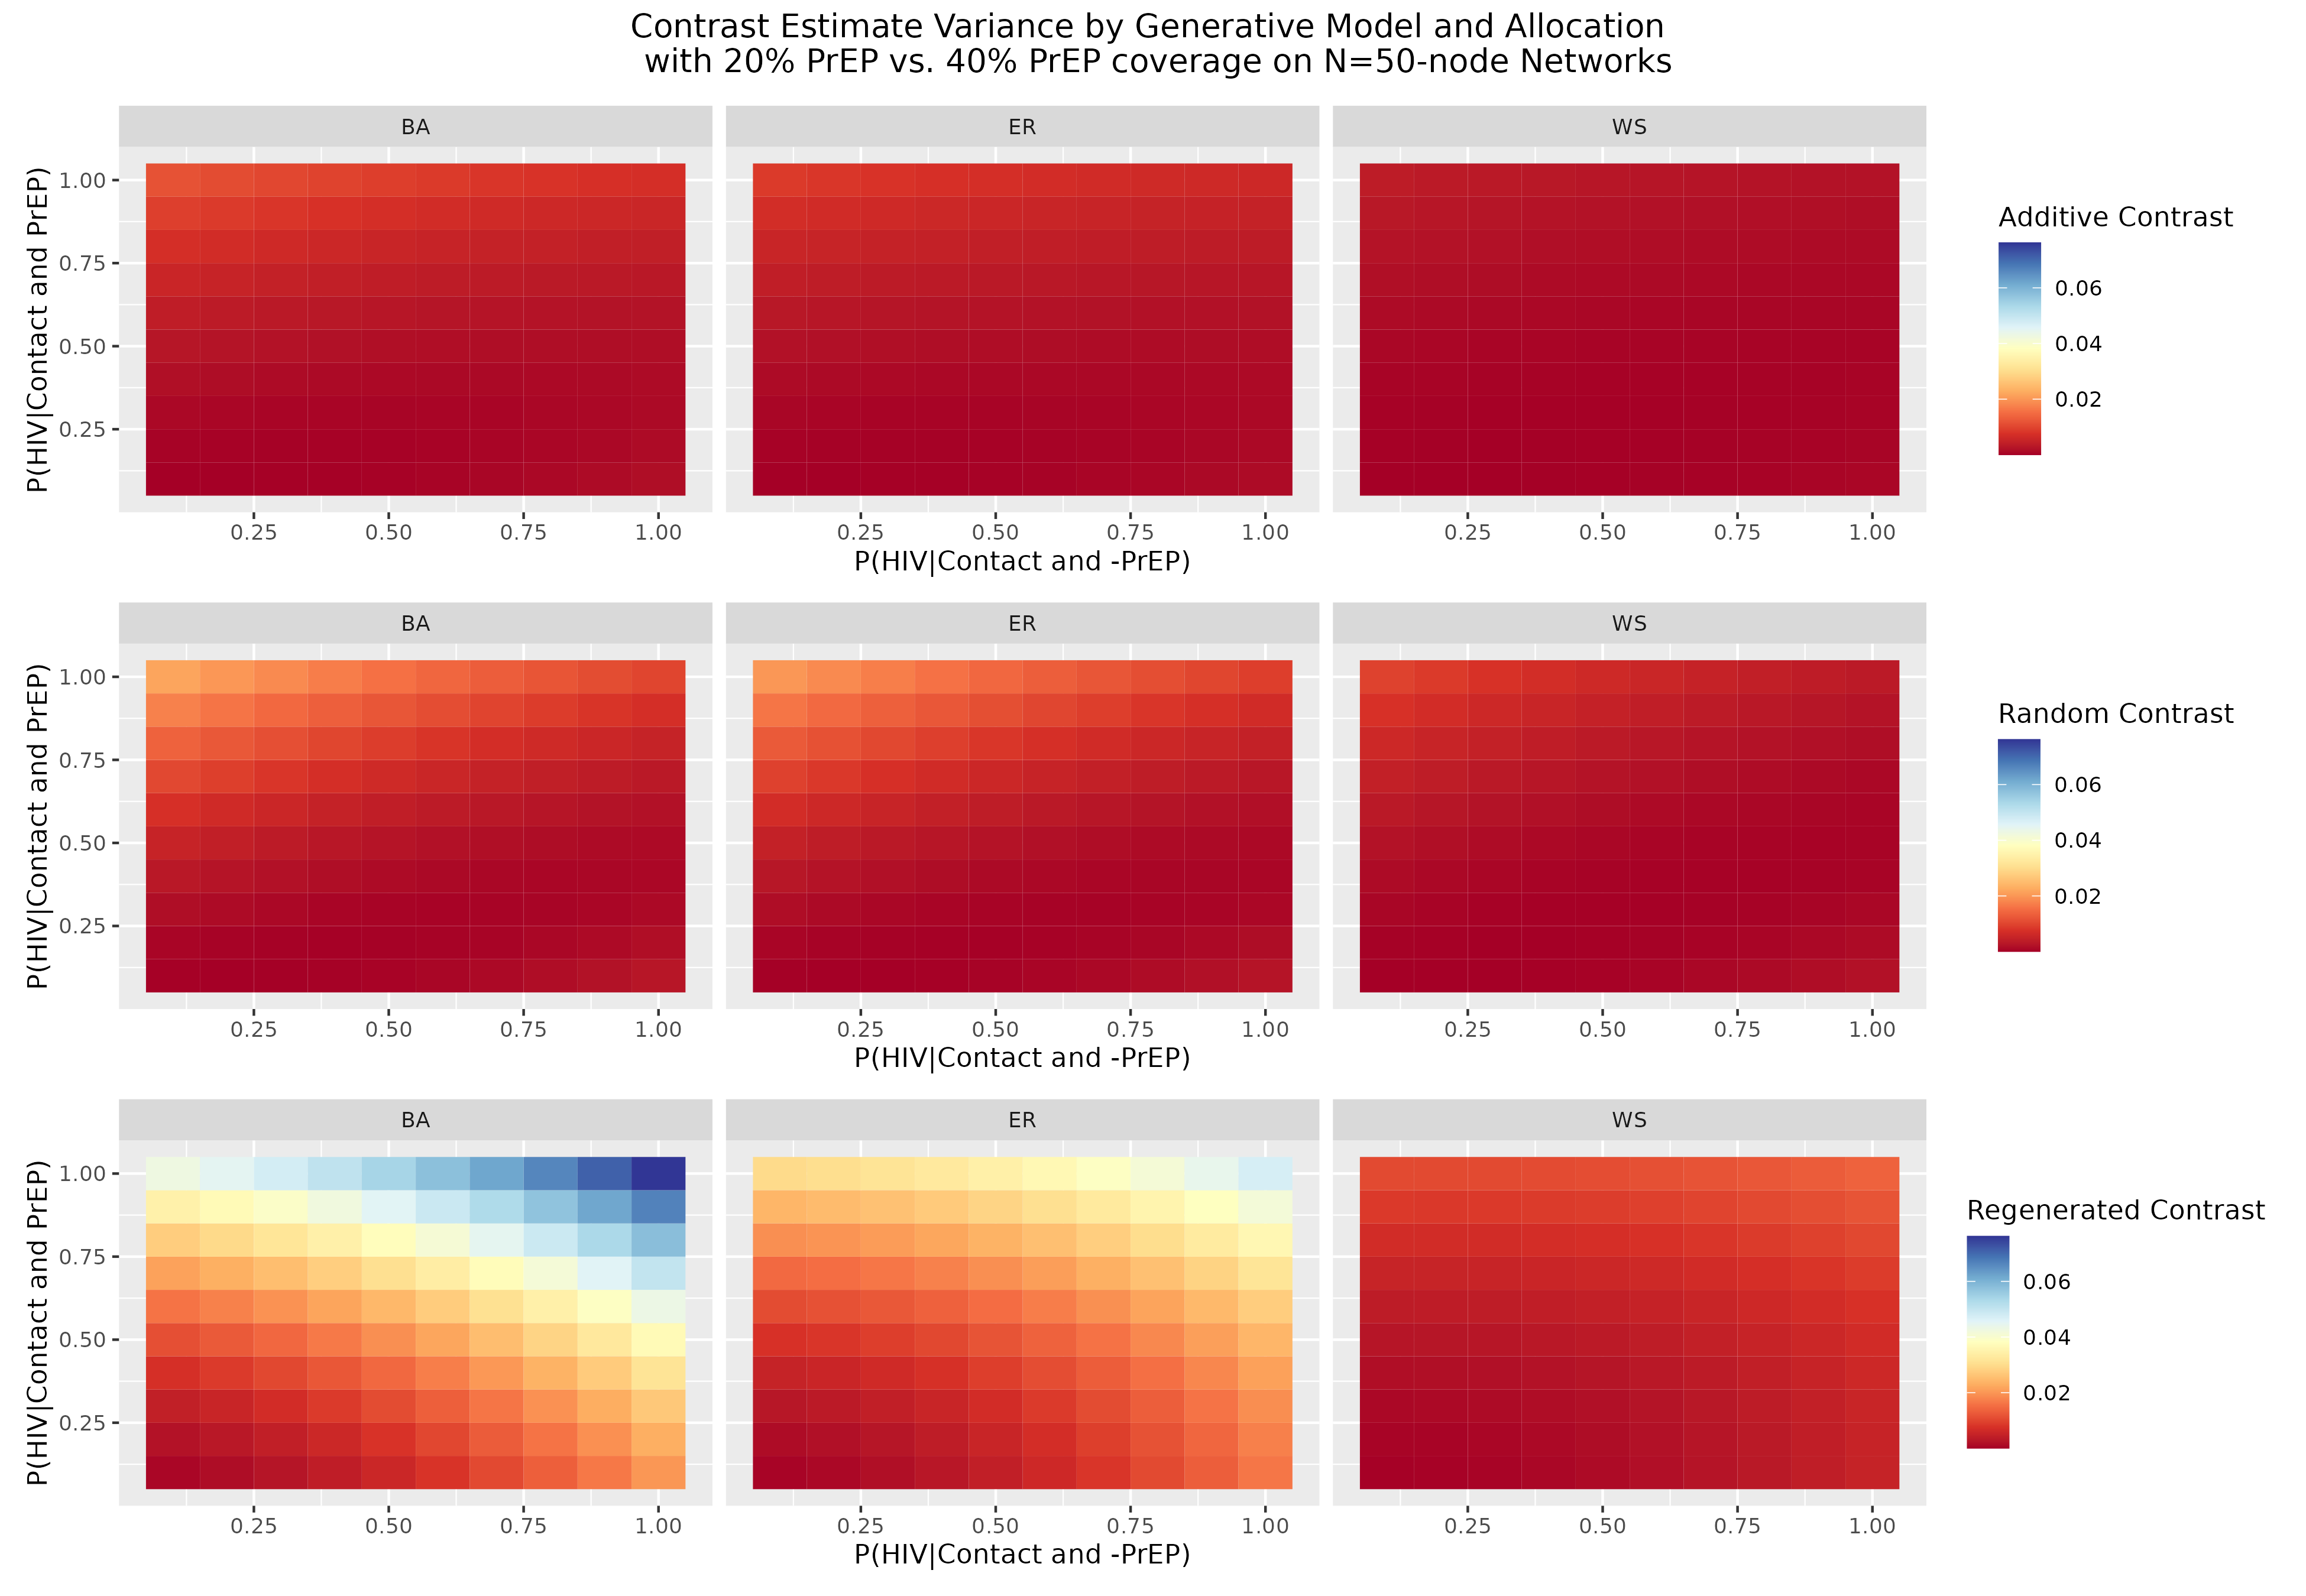
\includegraphics[width=\linewidth]{Corrected Figures/Generative Model Variance Plot.png}
    \caption{Variance of risk difference estimates comparing number of new infections when 40\% versus 20\% of uninfected nodes are treated with PrEP across varying levels of $\mathbb{P}\left[\text{HIV} \vert \neg \text{PrEP} \cap \text{Contact}\right]$ and $\mathbb{P}\left[\text{HIV} \vert \text{PrEP} \cap \text{Contact}\right]$, stratified by Network Generative Model with a Network Size of 50 and using 200 simulation samples %%PLEASE ADD%%. 
    From left to right, ``BA" the Barabási–Albert scale-free model, ``ER" the Erdős–Rényi Random Graph model, ``WS" the Watts-Strogatz Small-World model. From top to bottom: ``Additive" approach increases the proportion on PrEP compared to a given network realization and given set of treated nodes; ``Random" approach compares PrEP allocation levels for a given network realization, without fixing the treated nodes; ``Regenerated" approach compares PrEP levels without fixing network realization or treated nodes. 
    }
    \label{fig:Figure 12}
\end{figure}


\section{Discussion}

 When estimating causal effects using network-based simulation models, the exact pattern of network contacts is a potential source of bias because it determines the outcome and the potential range of causal effects under different treatment patterns applied to  that realization. The issue is structural -- the different networks have different interference patterns and as a result, the same intervention applied to different networks can have different effects (i.e., effect modification). But, if all other parameters are fixed, then increasing the number of runs or the network size could help, at least for some estimators (e.g., difference measures). More runs provide a more robust sample of the effect space, which decreases the bias, but a larger network changes the context of the causal question and pushes the true effect toward the null (assuming no other parameters are changed). Whenever a simulation study must use a finite number of network realizations but does not have a specific empiric network structure of interest, it is important that each counterfactual contrast be estimated on each network realization, then averaged across all realizations to reduce the impact of this bias. 

 In both our simplified example and our more complex simulations, we see that this potential for bias does affect our estimates when an inappropriate choice of network simulation approach is used.  For all model parameters considered, our simulations showed evidence of effect modification by network structure of the relationship between risks of HIV given infectious contact with and without PrEP treatment. This effect modification is a source of the bias in the estimated average overall effects when we do not estimate counterfactuals conditional on network realization, and also generally the (implicit) reason for using a network modeling approach. In our simulations, the impact of network parameters on the amount of bias aligned with our expectations based on the probability of informative network realizations, with small network sizes or small numbers of network iterations resulting in more bias and higher variance when using an incorrect modeling approach.

We focused on examples that considered only the first time step of the simulation, and as a result, the impact of interference in our analyses was minimal. Because of this, we chose to present only the average overall effect estimates. However, it is important to be aware that the bias described here is not restricted to the average overall effect. In fact, all causal effects for depending happenings are expected to be potentially vulnerable to this bias. As time in the simulation increases, there will generally be an increase in the number of people infected, and thus, the proportion of the population who are uninfected and treated and/or have an infectious contact will change. This will change the distribution of informative network realizations (those where at least one treated individual has an infectious contact), and the amount of expected bias when not conditioning on network realization will thus evolve over time. Our estimator for the probability of informative network realizations suggests that this evolution will be dependent on the relative changes between the number of infected individuals and the number of treated individuals, as well as whether the treatment patterns of interest allow additional treatment initiation options over time.



In comparison to prior approaches in the literature, ...

In future work, the optimal number of runs using a similar approach could provide an intuition about the probability of uninformative networks. We could also investigate these issues on the ratio or odds scale for the parameters.

Overall, when network-based causal effects are of interest, and the true network structure(s) is unknown so that the network must be simulated, we recommend that every simulated realization of the network be subjected to all treatment patterns under study so that network-specific causal effects can be estimated for each realization and then pooled across all simulated network realizations. This approach will ensure the smallest variance and least bias in the results for a given set of parameters and will often allow smaller or fewer network simulations to be run. In the rare case where the exact structure of the network of interest is known, the same approach is appropriate, except that the resulting causal effect estimate will be the average network-specific causal effect, not the average causal effect across all networks with the given parameter set.




\newpage

\bibliographystyle{unsrt}
\bibliography{references2}
\newpage


\appendix
\counterwithin{figure}{section}
\section{\textbf{Derivation of  \textit{P}}}
\label{Appendix 1}
Here we describe the details of the definition for the probabilities of an informative network structure $P$, the probability that a randomly generated network has at least one node $i$ assigned to treatment and with at least one infectious contact, for a given network parameter set and structure $j$, when $n$ individuals have infectious contact, and under a given treatment strategy $\alpha$ which results in $k$ expected treated individuals.

In the following calculation, we will be using the notation $f(x)\approx g(x)$ to mean that $f(x)=\Theta(g(x))$. Big theta notation is used to denote that there exists $M$ such that for $x>M$, there exist constants $c$ and $d$ such that:

 $$c\cdot g(x)< f(x) < d \cdot g(x) $$

It is easy to show that if $0<a<x<b$ and $0<c<y<d$, then $-d<-y<-c$ and $\frac{1}{d}<\frac{1}{y}<\frac{1}{c}$.  Therefore, $ac<xy<bd$ and $0<\frac{a}{d}<\frac{x}{y}<\frac{b}{c}$. It follows that if $f_1(x)=\Theta{\left(g_1(x)\right)}$ and $f_2(x)=\Theta{\left(g_2(x)\right)}$ where $f_1$,$f_2$, $g_1$ and $g_2$ are strictly positive then:
\begin{enumerate}
\item $f_1(x)f_2(x)=\Theta{\left(g_1(x)g_2(x)\right)}$
\item $\frac{f_1(x)}{f_2(x)}=\Theta{\left(\frac{g_1(x)}{g_2(x)}\right)}$
\end{enumerate}

\noindent In our notation, this can be written as:
\begin{enumerate}
     \item $f_1(x)f_2(x)\approx g_1(x)g_2(x)$ 
     \item $\displaystyle\frac{f_1(x)}{f_2(x)}\approx \frac{g_1(x)}{g_2(x)}$.
\end{enumerate}


\noindent Additionally, we will be using this version of Stirling's approximation \cite{robbins_remark_1955, zwillinger_6214_2002},

\begin{equation}
    \sqrt{2\pi n}\left(\frac{n}{e}\right)^{n}e^{\frac{1}{12n+1}} < n! < \sqrt{2\pi n}\left(\frac{n}{e}\right)^{n}e^{\frac{1}{12n}} \nonumber
\end{equation}

\noindent which implies that
$$n!= \Theta\left(\sqrt{2\pi n}\left(\frac{n}{e}\right)^n \right)$$


\noindent Note that the bounding constants can be brought arbitrarily close to 1.

Now, assume that there are $N$ in the network population at a given time point, that $k\ll N$ is the number of individuals that receive treatment, and that $n\ll N$ is the number of individuals with an infectious contact. Then, there are $\binom{N}{k}$ unique network configurations.
 
The expected number of unique network configurations in which all treated individuals have no infectious contacts (and thus a contribution of 0 to the effect estimate) is then given by $\binom{N-n}{k}$. Then, the proportion of network configurations in which at least one treated individual has at least one infectious contact is 
\begin{equation} 
\frac{{\binom{N}{k}}-{\binom{N-n}{k}}}{{\binom{N}{k}}}=1-\frac{{\binom{N-n}{k}}}{{\binom{N}{k}}}  \nonumber
\end{equation}
Expanding the RHS gives:
\begin{equation}
1-\frac{\left(N-n\right)!\left(N-k\right)!}{k!\left(N-n-k\right)!} \nonumber
\end{equation}
Using Stirling's Approximation as appropriate,
\begin{equation}
\approx 1-\frac{\sqrt{2\pi\left(N-n\right)}\left(\frac{N-n}{e}\right)^{N-n}\sqrt{2\pi\left(N-k\right)}\left(\frac{N-k}{e}\right)^{N-k}}{\sqrt{2\pi N}\left(\frac{N}{e}\right)^{N}\sqrt{2\pi \left(N-n-k\right)}\left(\frac{N-n-k}{e}\right)^{N-n-k}}     \nonumber
\end{equation}

\noindent or equivalently, 

\begin{equation} \label{eq:19}
\approx 1-\frac{\sqrt{2\pi \left(N-n\right)}}{\sqrt{2\pi N}}\cdot\frac{\sqrt{2 \pi \left(N-k\right)}}{\sqrt{2 \pi \left(N-n-k\right)}}\cdot\frac{\left(\frac{N-n}{e}\right)^{N-n}}
{\left(\frac{N}{e}\right)^{N}}\cdot\frac{\left(\frac{N-k}{e}\right)^{N-k}}{\left(\frac{N-n-k}{e}\right)^{N-n-k}}.    
\end{equation}
%see page 2b

\noindent Here we assume that if $f(x)=\Theta(g(x))$ then $1-f(x)=\Theta(1-g(x))$. This is not always the case but it holds here. Suppose that $0<a \cdot g(x)<f(x)<b \cdot g(x)$, $g(x)$ is bounded, and $a>1$ and $b>1$ can be made arbitrarily close to 1. This allows us to find $c$ and $d$ such that

$$c \cdot (1-g(x))<1-b\cdot g(x)< 1-f(x)<1-a\cdot g(x)<d \cdot (1-g(x))$$ 

\noindent In the following section, we will frequently make use of the fact that if $g(x)>0$ and $f(x)=\Theta{\left(g(x)h(x)\right)}$ then $f(x)=g(x)\Theta{\left(h(x)\right)}$. The proof of this is a straightforward application of the definition of $\Theta{\left(g(x)h(x)\right)}$.


 Considering each component of the product term in Equation \ref{eq:19} separately, we can perform several approximations and simplifications. The first component can be simplified in the following way:
\begin{equation}
    \frac{\sqrt{2\pi \left(N-n\right)}}{\sqrt{2\pi N}}=\sqrt{\frac{N-n}{N}}\approx 1 \text{ for } N \gg n \nonumber\\
    \end{equation}

\noindent The second component can be treated similarly:

\begin{equation}
    \frac{\sqrt{2 \pi \left(N-k\right)}}{\sqrt{2 \pi \left(N-n-k\right)}}\approx 1 \text{ for } N \gg n \text{ and } N \gg k \nonumber
\end{equation}
\noindent The third component requires a different approach:
    \begin{align}
    \frac{\left(\frac{\left(N-n\right)}{e}\right)^{N-n}}{{\left(\frac{N}{e}\right)^{N}}}&=\frac{\left(N-n\right)^{N-n}e^{N}}{N^{N}e^{N-n}} \nonumber\\
     &=\frac{e^{n}}{N^{n}}\left(\frac{N-n}{N}\right)^{N-n} \nonumber\\
     &=\frac{e^{n}}{N^{n}}\left(1-\frac{n}{N}\right)^{N-n} \nonumber\\
     &=\frac{e^{n}}{N^{n}}\frac{\left(1-\frac{n}{N}\right)^{N}}{\left(1-\frac{n}{N}\right)^{n}} \nonumber\\
     &\approx \frac{e^{n}}{N^{n}}\lim_{N \to \infty}\frac{\left(1-\frac{n}{N}\right)^{N}}{\left(1-\frac{n}{N}\right)^{n}} \nonumber\\
     &=\frac{e^{n}}{N^{n}}\frac{e^{-n}}{1^{n}} \nonumber\\
     &=\frac{1}{N^{n}} \nonumber
\end{align}
\noindent Finally, the fourth component is simplified as follows: 
\begin{align}
    \frac{\left(\frac{N-k}{e}\right)^{N-k}}{\left(\frac{N-n-k}{e}\right)^{N-n-k}}&\stackrel{M\coloneqq N-k}{=}\frac{\left(\frac{M}{e}\right)^{M}}{\left(\frac{M-n}{e}\right)^{M-n}}\to M^{n} \nonumber\\
    \frac{M^{n}}{N^{n}}&=\left(\frac{N-k}{N}\right)^{n}\nonumber
\end{align}
Putting this back together into Equation \ref{eq:19} and simplifying, we get the following estimator for the probability, $P$, of an informative network structure:
\begin{align}
    & \approx 1- \frac{\left(N-n\right)^{N-n}\left(N-k\right)^{N-k}}{N^{N}\left(N-n-k\right)^{N-n-k}} \nonumber\\
    &= 1- N^{-N}\left(\frac{N-n}{N}\right)^{N-n}\left(N-k\right)^{n}\left(\frac{N-k}{N-n-k}\right)^{N-n-k} \nonumber\\
    &=1-\left(\frac{N^{n}\left(1-\frac{n}{N}\right)^{N}\left(N-k\right)^{n}}{\left(1-\frac{n}{N}\right)^{n}}\right)\left(\frac{N-n-k}{N-k}\right)^{k+n-N} \nonumber\\
    &=1-\left(\frac{N^{-n}e^{-n}\left(N-k\right)^{n}}{1}\right)\left(\frac{\left(1-\frac{n}{N-k}\right)^{n}}{\left(1-\frac{n}{N-k}\right)^{N-k}}\right) \nonumber\\
    &=1-\frac{N^{-n}\left(N-k\right)^{n}e^{-n}}{e^{-n}} \nonumber\\
    &=1-\frac{\left(N-k\right)^{n}}{N^{n}} \nonumber\\
    &=1-\left(\frac{N-k}{N}\right)^{n}.\nonumber
\end{align}

This estimator can be rewritten $P=1-(1-\frac{k/N})^n$. In this form, we can see these similarities to the binomial probability model for transmission\cite{becker_general_1981}. That model assumes a constant per-contact transmission probability, $p$, to estimate the probability of at least one transmission event across $m$ contact events as $(1-(1-p)^m$. Comparing this to our estimator for informative networks $P$, we see that the proportion of the population treated replaces the per-contact transmission probability, while the number of uninfected individuals with infectious contacts substitutes for the number of contact events.

\newpage

\section{\textbf{Network Summary Statistics}}
\label {Appendix 2}
\subsection{Definitions}
\begin{definition}[Connected Components]
A connected component of a graph $G=(V,E)$ is a subgraph $G'=(V' \subseteq V,E' \subseteq E)\subseteq G$ such that there exists a path between any two nodes in $V'$.
\end{definition}
\begin{definition}[Betweenness Centrality]
The Betweenness Centrality for a node $v$ is given by: $$g(v)=\sum_{s\neq t\neq v}\frac{\sigma_{s,t}(v)}{\sigma_{s,t}},$$ where $\sigma(s,t)$ is  the number of shortest paths between node s and node t, and  $\sigma_{s,t}(v)$ is the number of shortest paths between node $s$ and node $t$ containing the node $v$ \cite{barabasi_network_2016}.
\end{definition}
\begin{definition}[Edge Density]
The (edge) density of a graph is the proportion of possible edges between nodes
that are actually present in the graph.
\end{definition}
\begin{definition}[Geodesic distance]
The geodesic distance between two nodes is the length of the shortest path between them.
\end{definition}
\begin{definition}[Graph diameter]
The diameter of a graph or graph component is the largest path length between any two nodes is the graph (component).
\end{definition}
\begin{definition}[Transitivity]
Transitivity is the proportion of closed triangles in a graph.
\end{definition}
\begin{definition}[$k$-core decomposition]
A $k$-core of a graph is a subgraph in which all nodes are connected to at least $k$ other nodes in the subgraph.
\end{definition}

\subsection{Results by Network Model}
\begin{figure}[H]
    \centering
    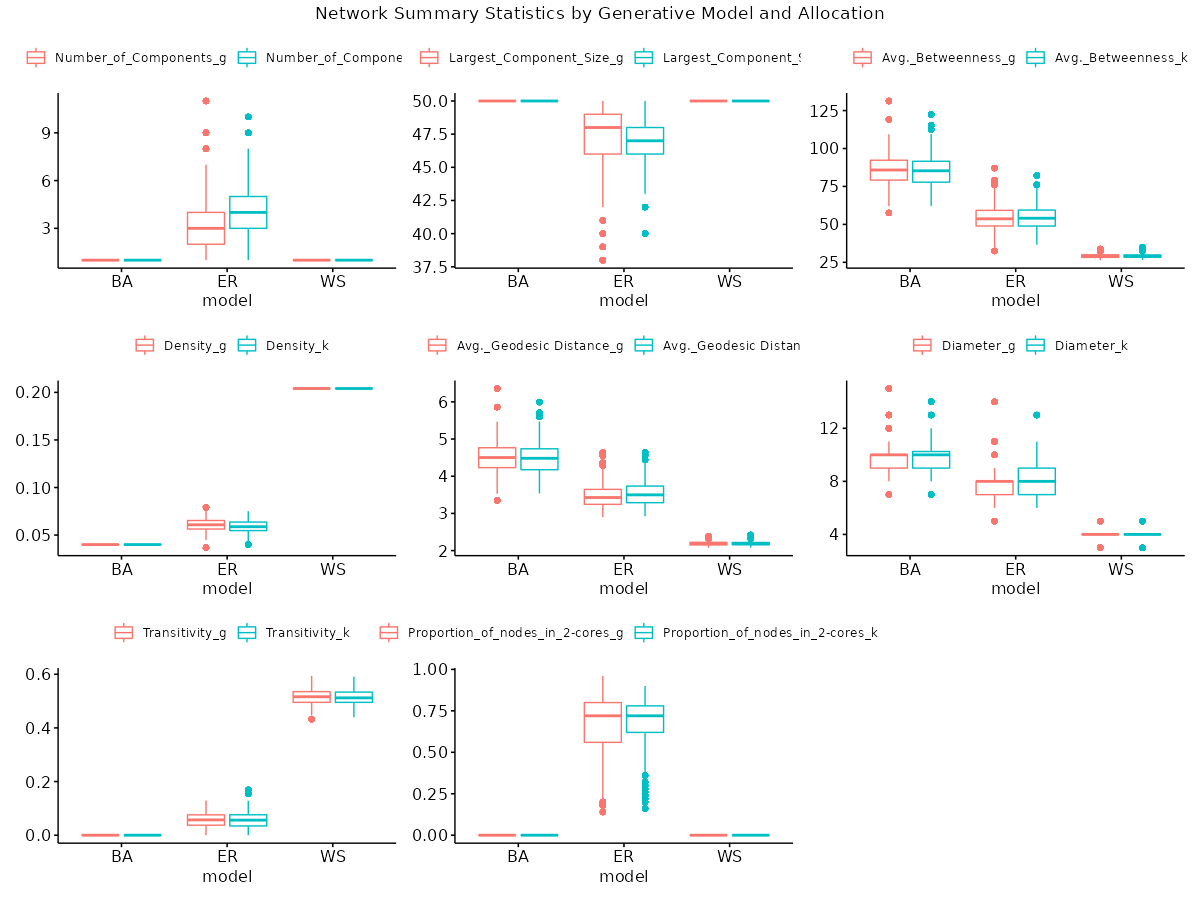
\includegraphics[width=\linewidth]{Corrected Figures/Network Summary Statistics.png}
    \caption{Select Network Summary Statistics by Network Generative Model}
    \label{fig:Figure B1}
\end{figure}

The network summary statistics in \ref{fig:Figure B1} for each network model confirm the characteristics we expect for each generative model. Barabási–Albert and Watts-Strogatz both have a single connected component, as they are connected graphs by design. The number of connected components in Erdős–Rényi model graphs varies widely. The sizes of the largest component are equivalent to the graph order in Barabási–Albert  and Watts-Strogatz models but are variable in Erdős–Rényi models. Watts-Strogatz models have shorter average path lengths than Erdős–Rényi models, thus betweenness centrality for any given node decreases. Watts-Strogatz models are designed to have high clustering and short average path lengths, and this is reflected in high values of edge density and transitivity (also called global clustering) with relatively low geodesic distance and diameter. By contrast, the preferential attachment and power-law degree distribution of Barabási–Albert graphs results in relatively low density and transitivity and relatively high diameter. As connected graphs, the Watts-Strogatz and Barabási–Albert models do not have meaningful $k$-core decompositions, so the 2-core proportions are identically zero for both.



\section{\textbf{Algorithm for simulating the average overall effect on networks}}
\label{Appendix 3}

    \begin{enumerate}
\item In each simulation iteration, let $G_{\text{control}}=\left(V_{\text{control}},E_{\text{control}}\right)$ be the ``control" network graph, with $\vert V_{\text{control}}\vert \eqqcolon N_{\text{control}}$. The vertex attributes of $V_{\text{control}}$ are initialized to one of three states: 
\begin{itemize}
        \item  $N_{HIV}(V_{\text{control}})=N_{\text{control}}p_{hiv}$ nodes are initialized to the  ``infectious" state.
        \item $N_{PrEP_{1}}\left(V_{\text{control}}\right)=\left[N_{\text{control}}-N_{HIV}\left(V_{\text{control}}\right)\right]p_{PrEP_{1}}$ nodes are initialized to the ``treated,susceptible" state. 
        \item The remaining $N_{\text{control}}-\left[N_{HIV}\left(V_{\text{control}}\right)+N_{PrEP_{1}}\left(V_{\text{control}}\right)\right]$ nodes are initialized to the ``untreated, susceptible" state.
    \end{itemize}
    \item The set $IC(V_{\text{control}})$ of susceptible nodes with at least one infectious contact is identified from each node's neighborhood.
    \item The probability of HIV given treatment in the control scenario, $\mathbb{P}(\text{HIV} \vert \text{PrEP})_{\text{control}}$ is computed:
    \begin{enumerate}
     
    \item We compute $\mathbb{P}\left( \text{PrEP} \cap \text{Infectious contact}\right)$ as the proportion of the treated set  $T(V_{\text{control}})$ that have an infectious contact: \begin{equation}
        \mathbb{P}\left( \text{PrEP} \cap \text{Infectious contact}\right)=\frac{\vert IC\left(V_{\text{control}}\right) \bigcap \left({T\left(V_{\text{control}}\right)}\right)\vert}{\vert T\left(V_{\text{control}}\right)\vert}.\nonumber
    \end{equation}
    \item The probability $\mathbb{P}\left(\text{HIV} \vert \text{PrEP}\right)_{\text{control}}$ is then 
    \begin{equation}
        \mathbb{P}\left(\text{HIV} \vert \text{PrEP}\right)_{\text{control}}=\mathbb{P}\left(\text{HIV} \vert \text{PrEP} \cap \text{Infectious Contact}\right) \mathbb{P}\left(\text{PrEP} \cap \text{Infectious Contact}\right)\nonumber
    \end{equation}
    \end{enumerate}
    \item We then similarly compute the probability of HIV given no treatment in the control scenario, $\mathbb{P} \left(\text{HIV} \vert \neg \text{PrEP}\right)_{\text{control}}$:
    \begin{enumerate}
    \item We compute $\mathbb{P}\left(\neg \text{PrEP} \cap \text{Infectious Contact} \right)  $ as the proportion of untreated susceptible nodes that have an infectious contact:
    \begin{equation}
        \mathbb{P}\left(\neg \text{PrEP} \cap \text{Infectious Contact} \right)=\frac{\vert IC\left(V_{\text{control}}\right) \bigcap \left({T'\left(V_{\text{control}}\right)}\right)\vert}{\vert T'\left(V_{\text{control}}\right)\vert},\nonumber
    \end{equation}

    where $T'\left(V_{\text{control}}\right)$ denotes the set of untreated susceptible nodes.
    \item The probability $\mathbb{P}\left(\text{HIV} \vert \neg \text{PrEP}\right)_{\text{control}}$ is then
    \begin{equation}
        \mathbb{P}\left(\text{HIV} \vert \neg \text{PrEP}\right)_{\text{control}}=\mathbb{P}\left(\text{HIV} \vert \neg \text{PrEP} \cap \text{Infectious Contact}\right) \mathbb{P}\left( \neg \text{PrEP} \cap \text{Infectious Contact}\right).\nonumber
    \end{equation}
    \end{enumerate}
    \item For the ``random" and ``additive" $\text{PrEP}_{2}$ treatment allocation  scenarios, the topology of $G_{\text{control}}$ is fixed, but treatment attributes on the vertex set are varied. 
    \begin{enumerate}
        \item For the ``random" $\text{PrEP}_{2}$ scenario, the infectious nodes from the control scenario are fixed, but the treatment set is instead a randomly selected $N_{\text{control}}PrEP_{2}$ nodes.
        %check me %
        \item For the ``additive" scenario, the infectious nodes are fixed, with the treated set $T\left(V_{\text{additive}}\right)$ contains the original treated nodes in addition to $\left[N_{\text{control}}-N_{HIV}-N_{PrEP1}\right]PrEP_{2}$ treated nodes.
    \end{enumerate}
    \item For the ``regenerated" treatment scenario, a new graph $G_{\text{regenerated}}=\left(V_{ \text{regenerated}},E_{\text{regenerated}}\right)$ with new attributes on the vertex set is generated.
    \begin{itemize}
        \item $N_{HIV}\left(V_{\text{regenerated}}\right)p_{hiv}$ nodes are assigned to the ``infectious" state.
        \item $N_{PrEP_{2}}\left(V_{\text{regenerated}}\right)=\left[N_{\text{regenerated}}\left(V_{\text{regenerated}}\right)-N_{HIV}\left(V_{\text{regenerated}}\right)\right]p_{PrEP_{2}}$ nodes are assigned to the ``susceptible, treated" state. 
    \end{itemize}
    \item The probabilities of infection with and without treatment are then computed similarly to the control scenario.
    \item The combined probability of HIV is computed, given each PrEP coverage and allocation
    \item The contrast estimate between each of the counterfactual allocations (``random", ``additive", ``regenerated") and the control are computed as the difference  between each of these combined probabilities and that for the control.
    \item These simulations are repeated $n_{sim}$ times and the means of these contrast estimates are computed.
\end{enumerate}


\section{\textbf{Example Annotated Networks for all Generative Models}}
\label{Appendix 4}
This appendix reproduces example networks for all generative models, demonstrating the relationship between the control network and the random and additive simulation approach for the intervention networks, compared to the regenerated network approach. Notice that when using the Watts-Strogatz model, the small-world connectivity makes it somewhat more challenging to see the differences between the Regenerated approach and the Random and Additive approaches. Nevertheless, close inspection will reveal that the specific connectivity patterns do indeed change in the Regenerated network.

\newpage
\begin{figure}
    \centering
    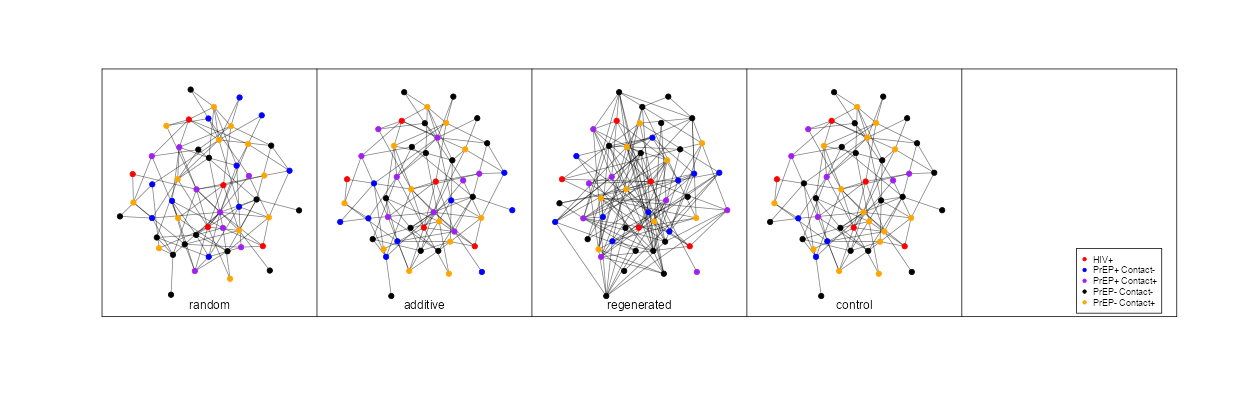
\includegraphics[width=\linewidth]{Original Figures/ER Network Example.png}
    \caption{Annotated Example ER Network showing color-coded treatment and disease states by network (control vs. regenerated) and allocation strategy(control vs. random, additive)}
    \label{fig: D1}
\end{figure}
\begin{figure}[H]
    \centering
    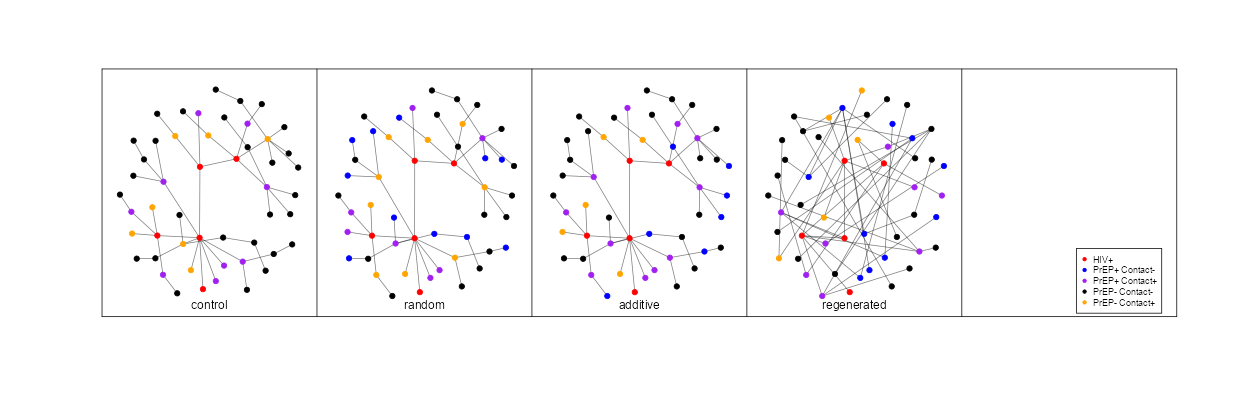
\includegraphics[width=\linewidth]{Original Figures/BA Network Example.png}
    \caption{Annotated Example BA Network showing color-coded treatment and disease states by network (control vs. regenerated) and allocation strategy(control vs. random, additive)}
    \label{fig: D2}
\end{figure}
\begin{figure}[H]
    \centering
    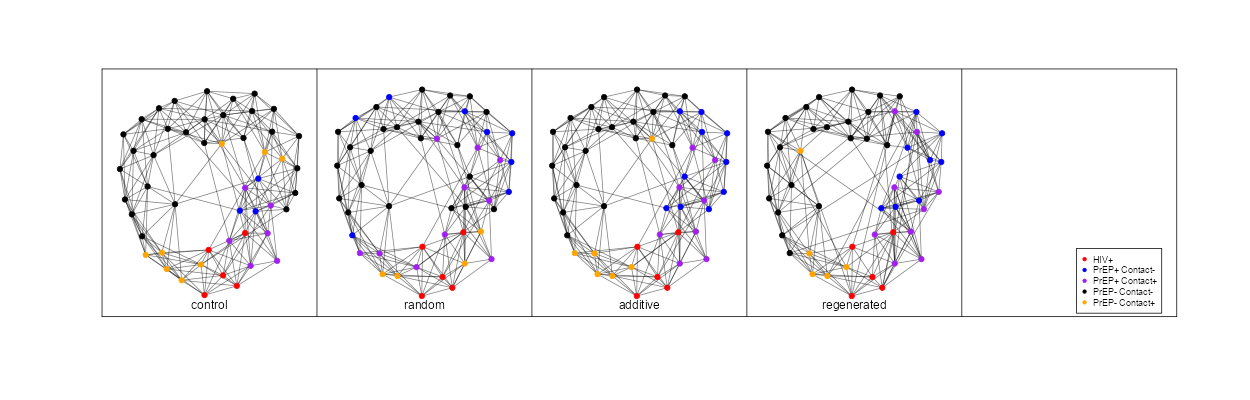
\includegraphics[width=\linewidth]{Original Figures/WS Network Example.png}
    \caption{Annotated Example WS Network showing color-coded treatment and disease states by network (control vs. regenerated) and allocation strategy (control vs. random, additive)}
    \label{fig: D3}
\end{figure}

\section{\textbf{Simulation model results across all input parameter and model type variations}}
\label{Appendix 5}

\subsection{Erdős–Rényi  Random Graph Models}

\subsubsection{Effect Modification by Network Size}
\begin{figure}[H]
    \centering
    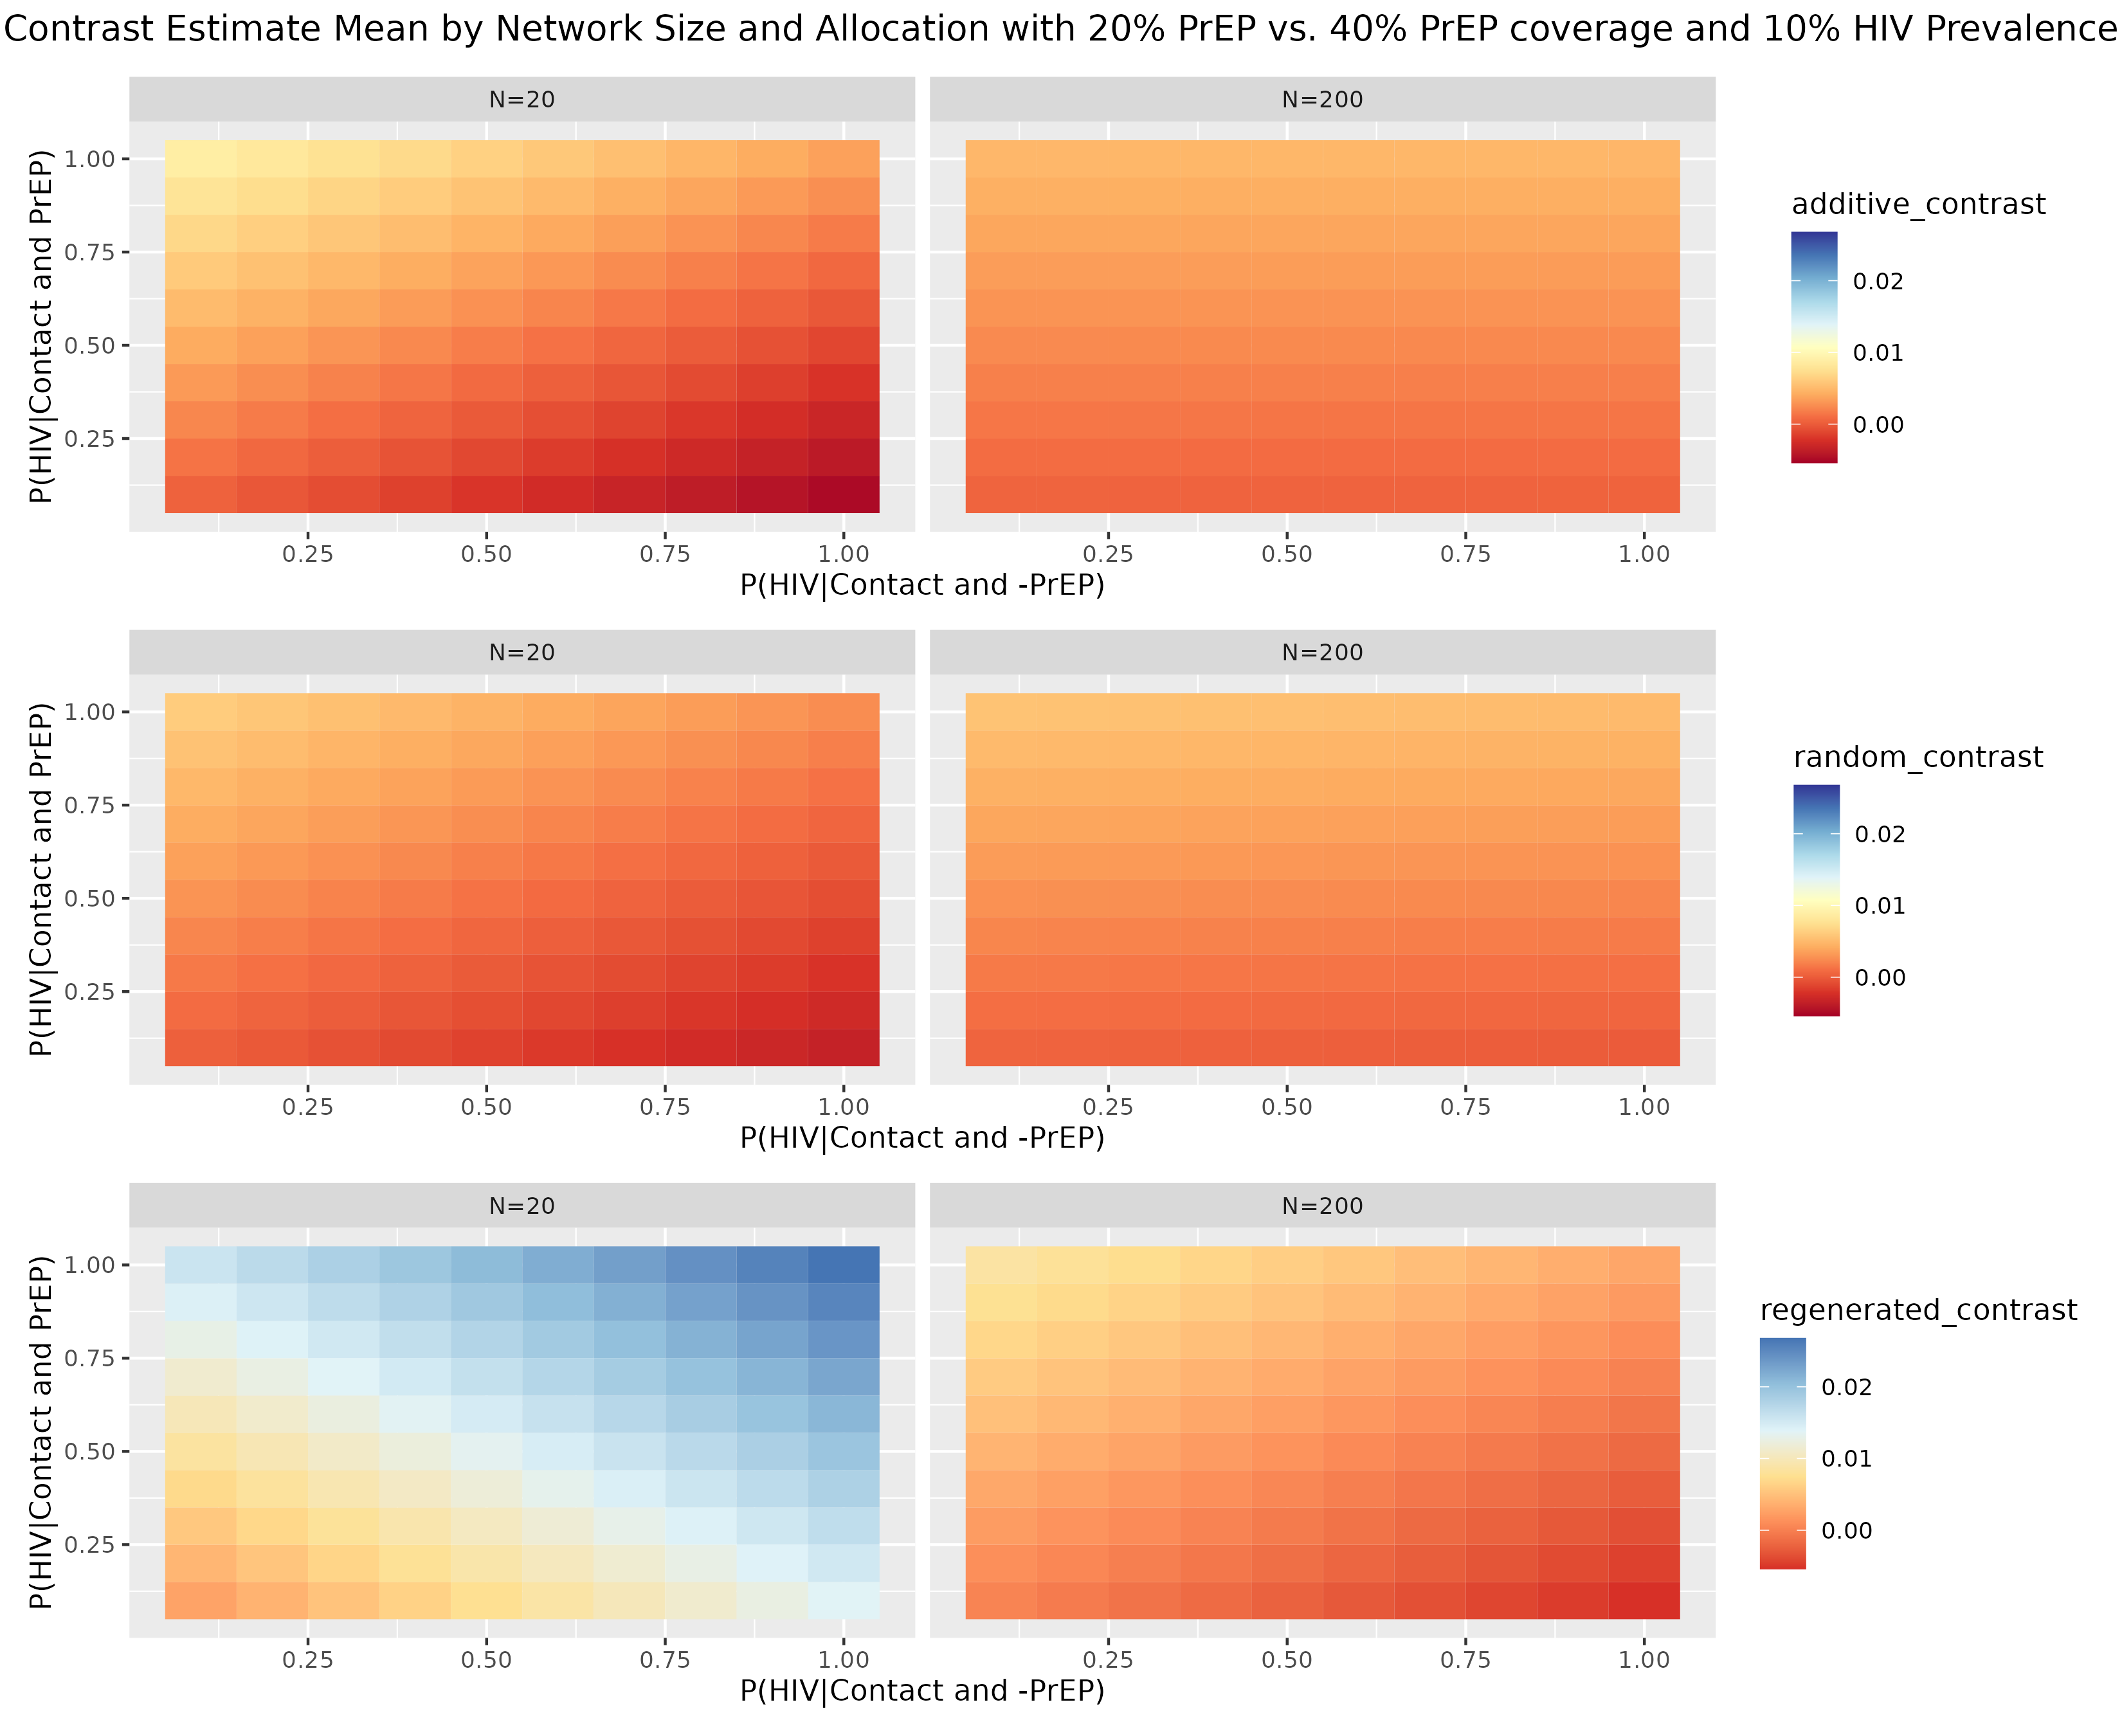
\includegraphics[width=\linewidth]{Corrected Figures/Network Size Mean Plot.png}
    \caption{Mean Causal Contrast estimates as $\mathbb{P}\left[\text{HIV} \vert \neg \text{PrEP} \cap \text{Contact}\right]$ and $\mathbb{P}\left[\text{HIV} \vert \text{PrEP} \cap \text{Contact}\right]$ increase, stratified by Network Size/Graph Order. From top to bottom: ``additive" Mean Contrast of random 20\% additional vs. random 20\% PrEP allocation control, ``random" Mean Contrast of random 40\% PrEP allocation vs. random 20\% control, ``regenerated" Mean Contrast of random 40\% allocation on regenerated network vs. random 20\% control. }
    \label{fig: Figure S4.1}
\end{figure}
\begin{figure}[H]
    \centering
    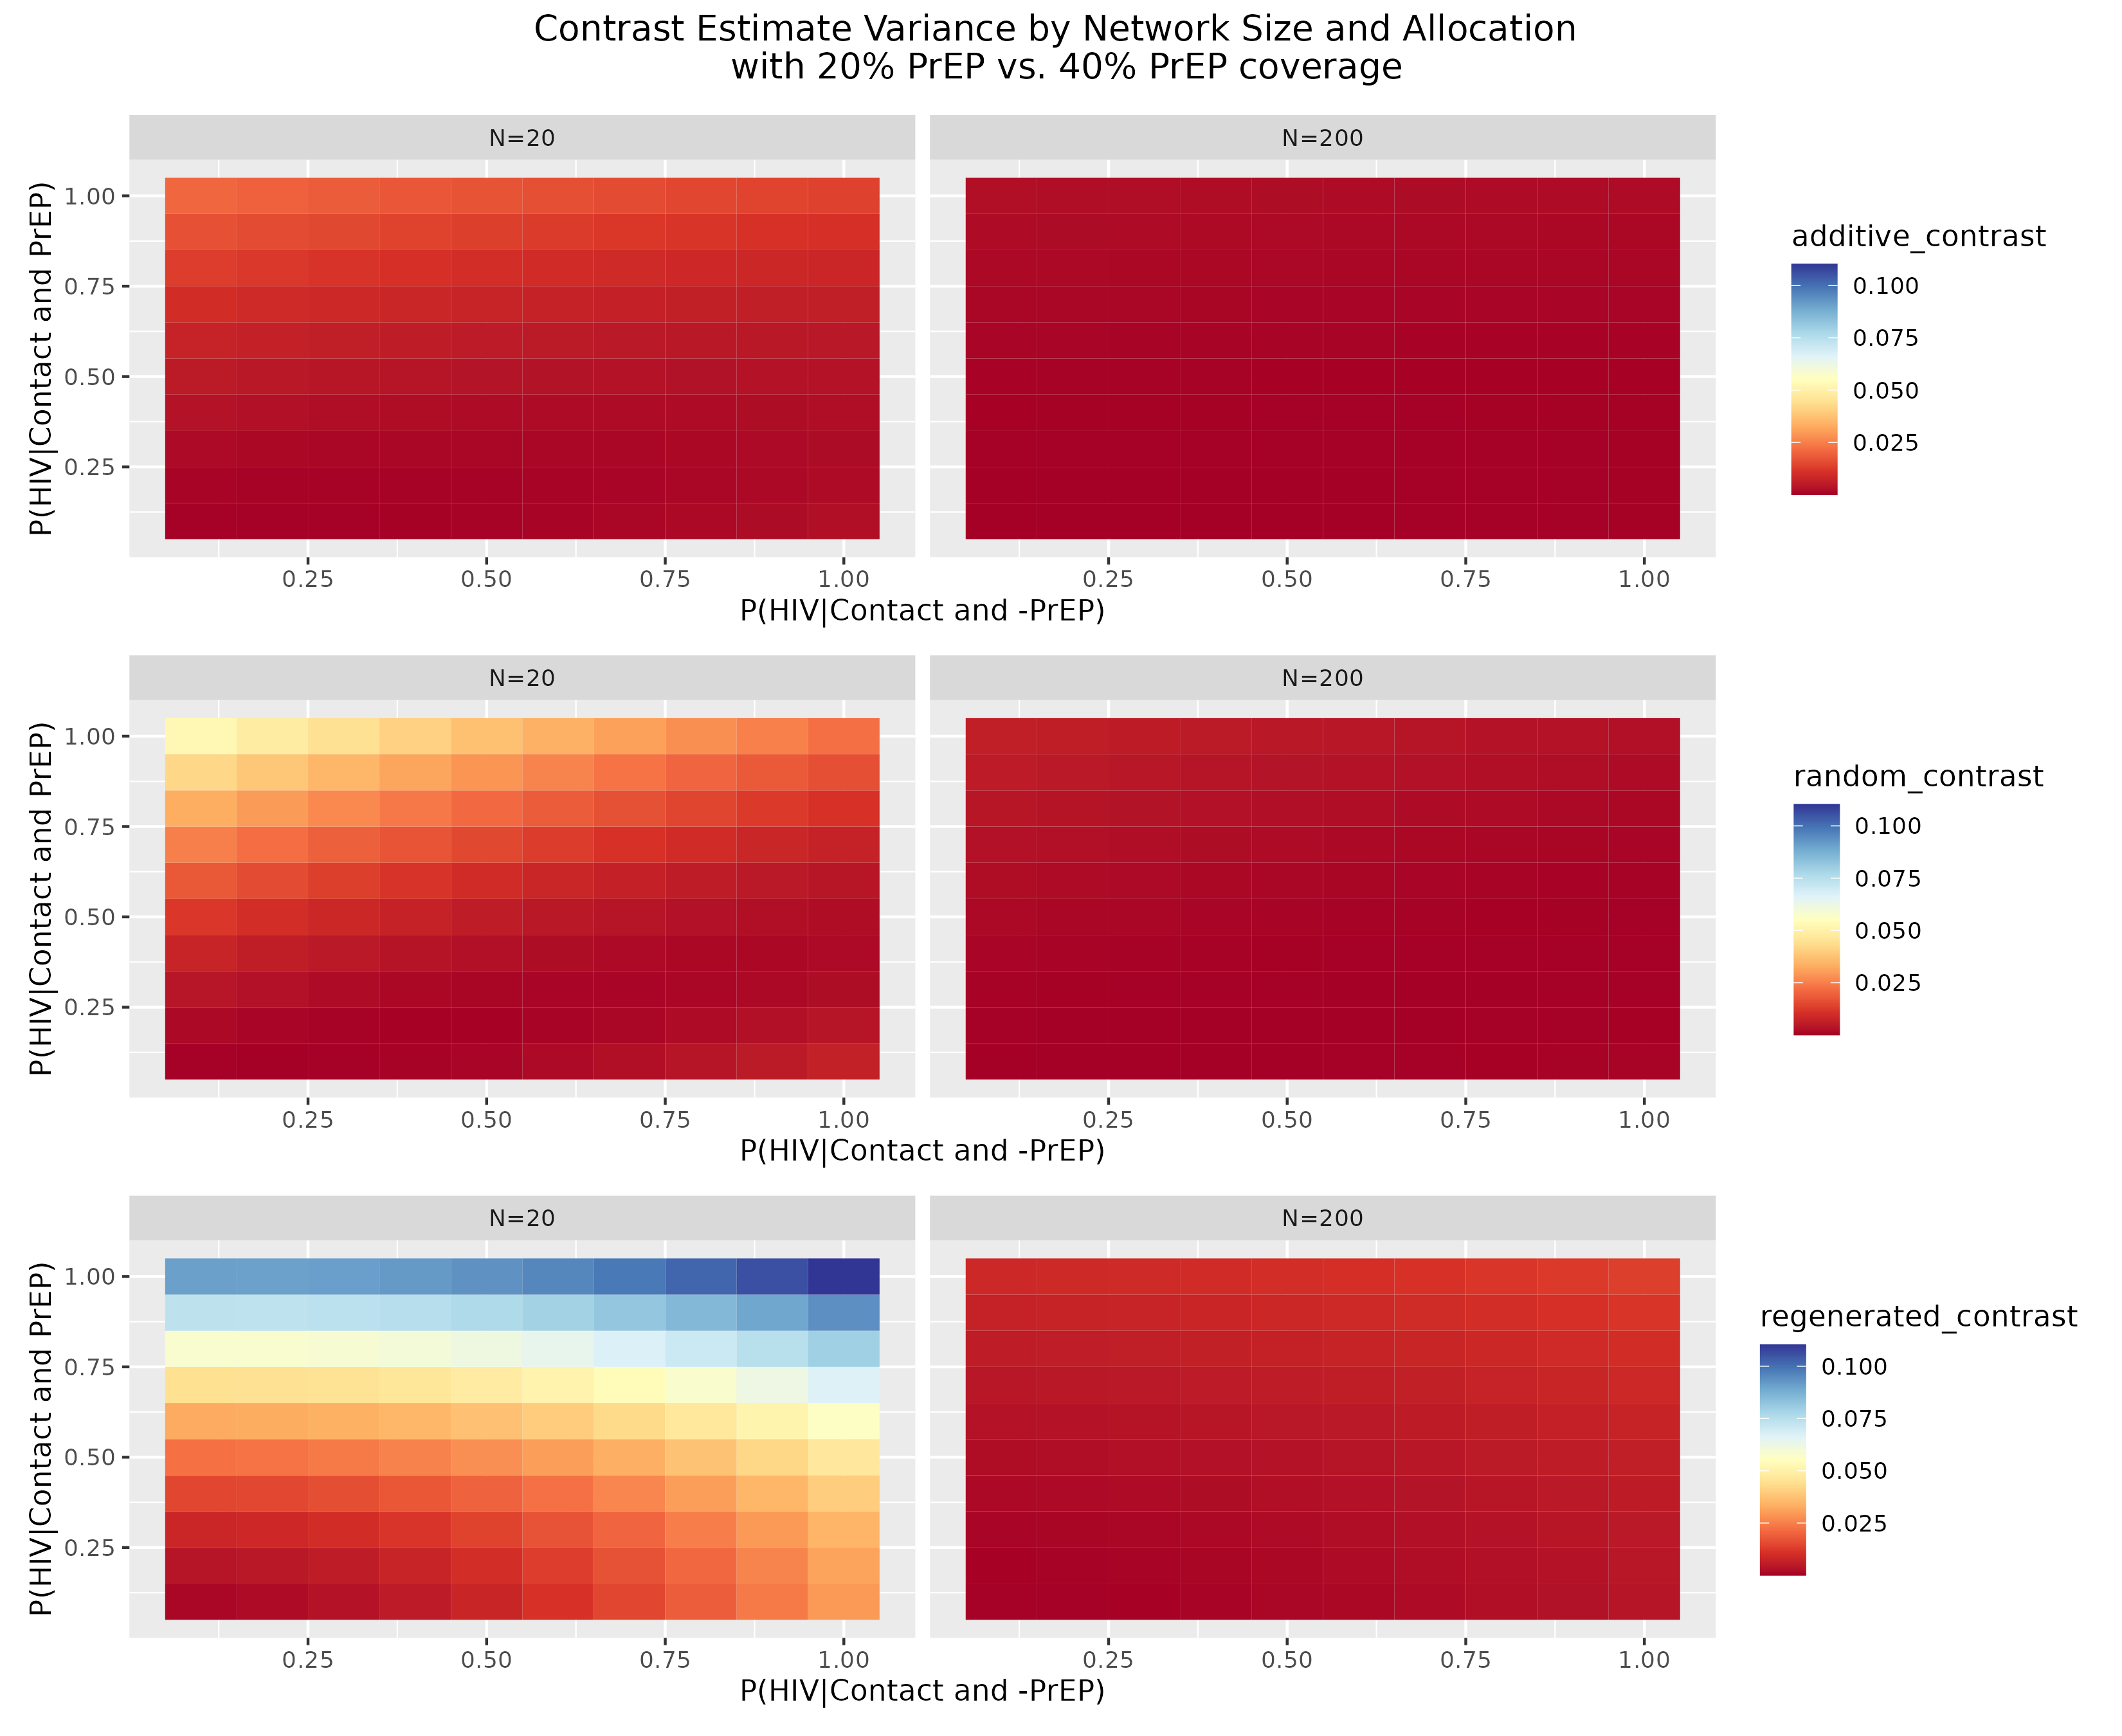
\includegraphics[width=\linewidth]{Corrected Figures/Network Size Variance plots.png}
    \caption{Variance of Causal Contrast estimates  as $\mathbb{P}\left[\text{HIV} \vert \neg \text{PrEP} \cap \text{Contact}\right]$ and $\mathbb{P}\left[\text{HIV} \vert \text{PrEP} \cap \text{Contact}\right]$ increase, stratified by Network Size/Graph Order. From top to bottom: ``additive" Variance of Contrast of random 20\% additional vs. random 20\% PrEP allocation control, ``random" Variance of Contrast of random 40\% PrEP allocation vs. random 20\% control, ``regenerated" Variance of Contrast of random 40\% allocation on regenerated network vs. random 20\% control.}
    \label{fig:Figure S4.2}
\end{figure}
From both the Mean and Variance plots above, there is an apparent effect modification of the relationship between the ``risks" of HIV and treatment allocation strategy at small network sizes. However, this modification essentially disappears in (order of magnitude) larger networks. The effect modification is particularly apparent with respect to the regenerated networks where the means are most variable across risk combinations (as well as the variances themselves).  

\subsubsection{Effect Modification by Resampling Sample Size}
\begin{figure}[H]
    \centering
    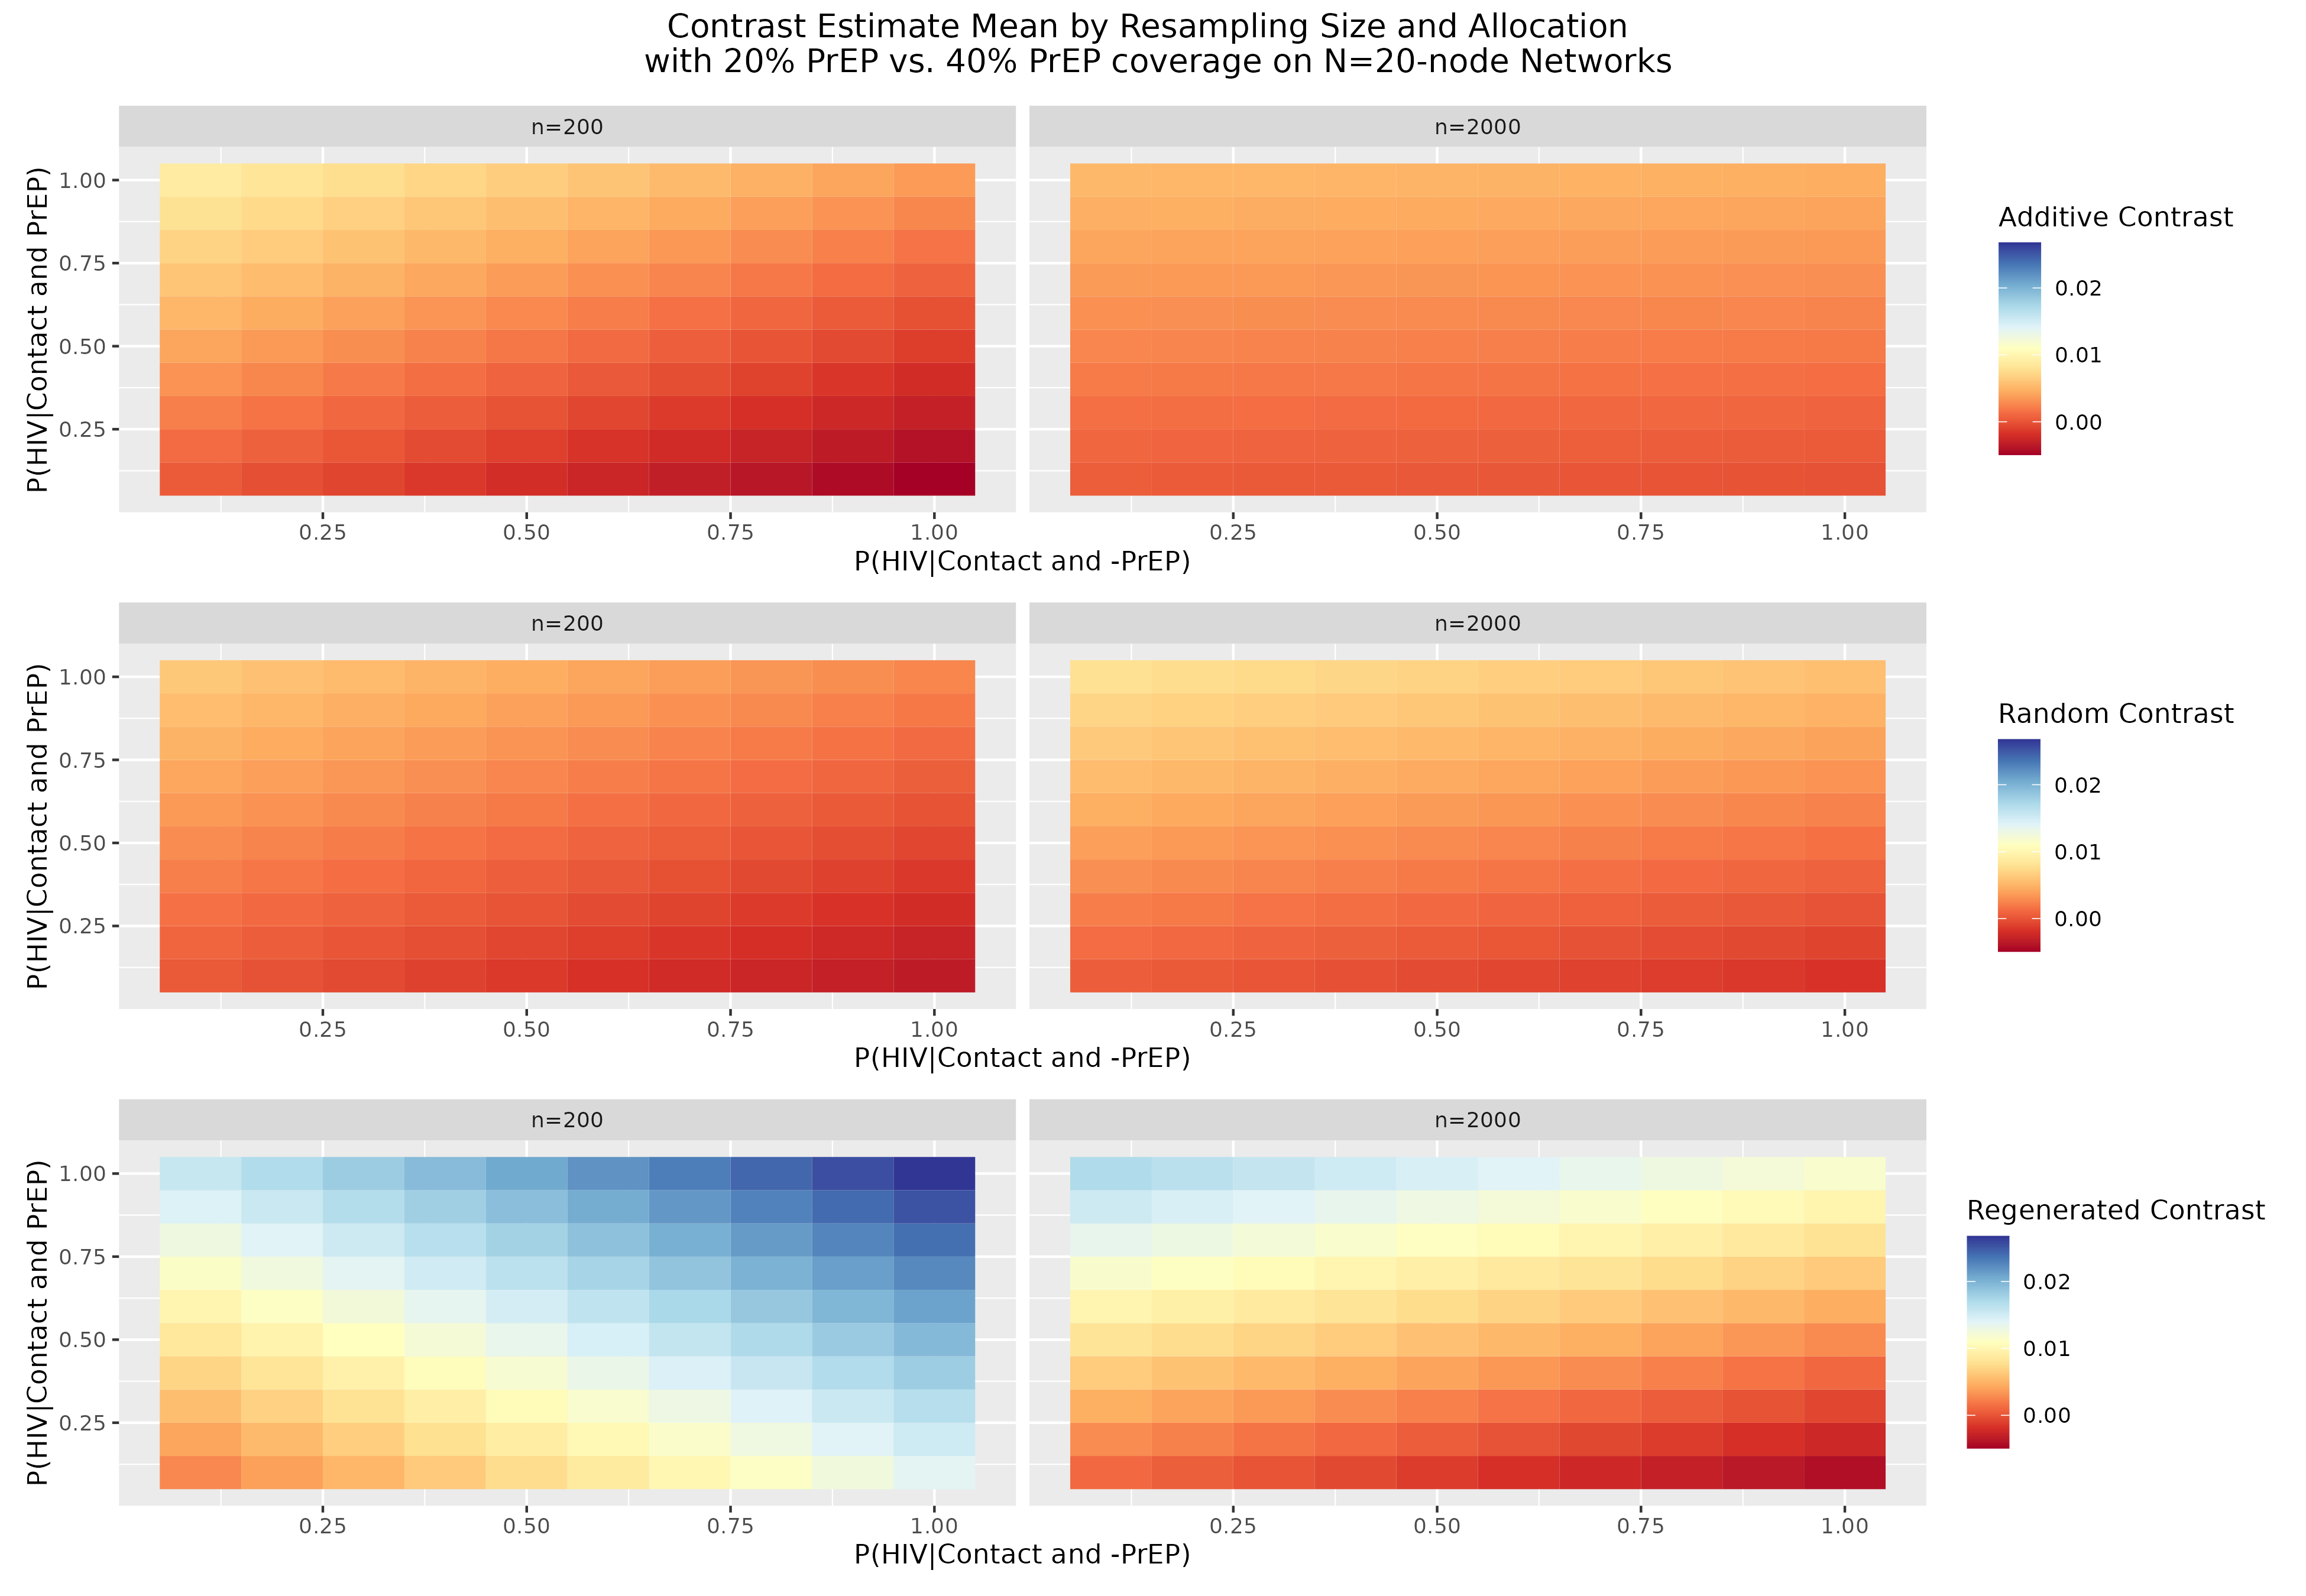
\includegraphics[width=\linewidth]{Corrected Figures/Resampling Size Mean Plot.png}
    \caption{Mean Causal Contrast estimates as $\mathbb{P}\left[\text{HIV} \vert \neg \text{PrEP} \cap \text{Contact}\right]$ and $\mathbb{P}\left[\text{HIV} \vert \text{PrEP} \cap \text{Contact}\right]$ increase, stratified by resampling sample size. From top to bottom: ``additive" Mean Contrast of random 20\% additional vs. random 20\% PrEP allocation control, ``random" Mean Contrast of random 40\% PrEP allocation vs. random 20\% control, ``regenerated" Mean Contrast of random 40\% allocation on regenerated network vs. random 20\% control.}
    \label{fig:Figure S4.3}
\end{figure}
\begin{figure}[H]
    \centering
    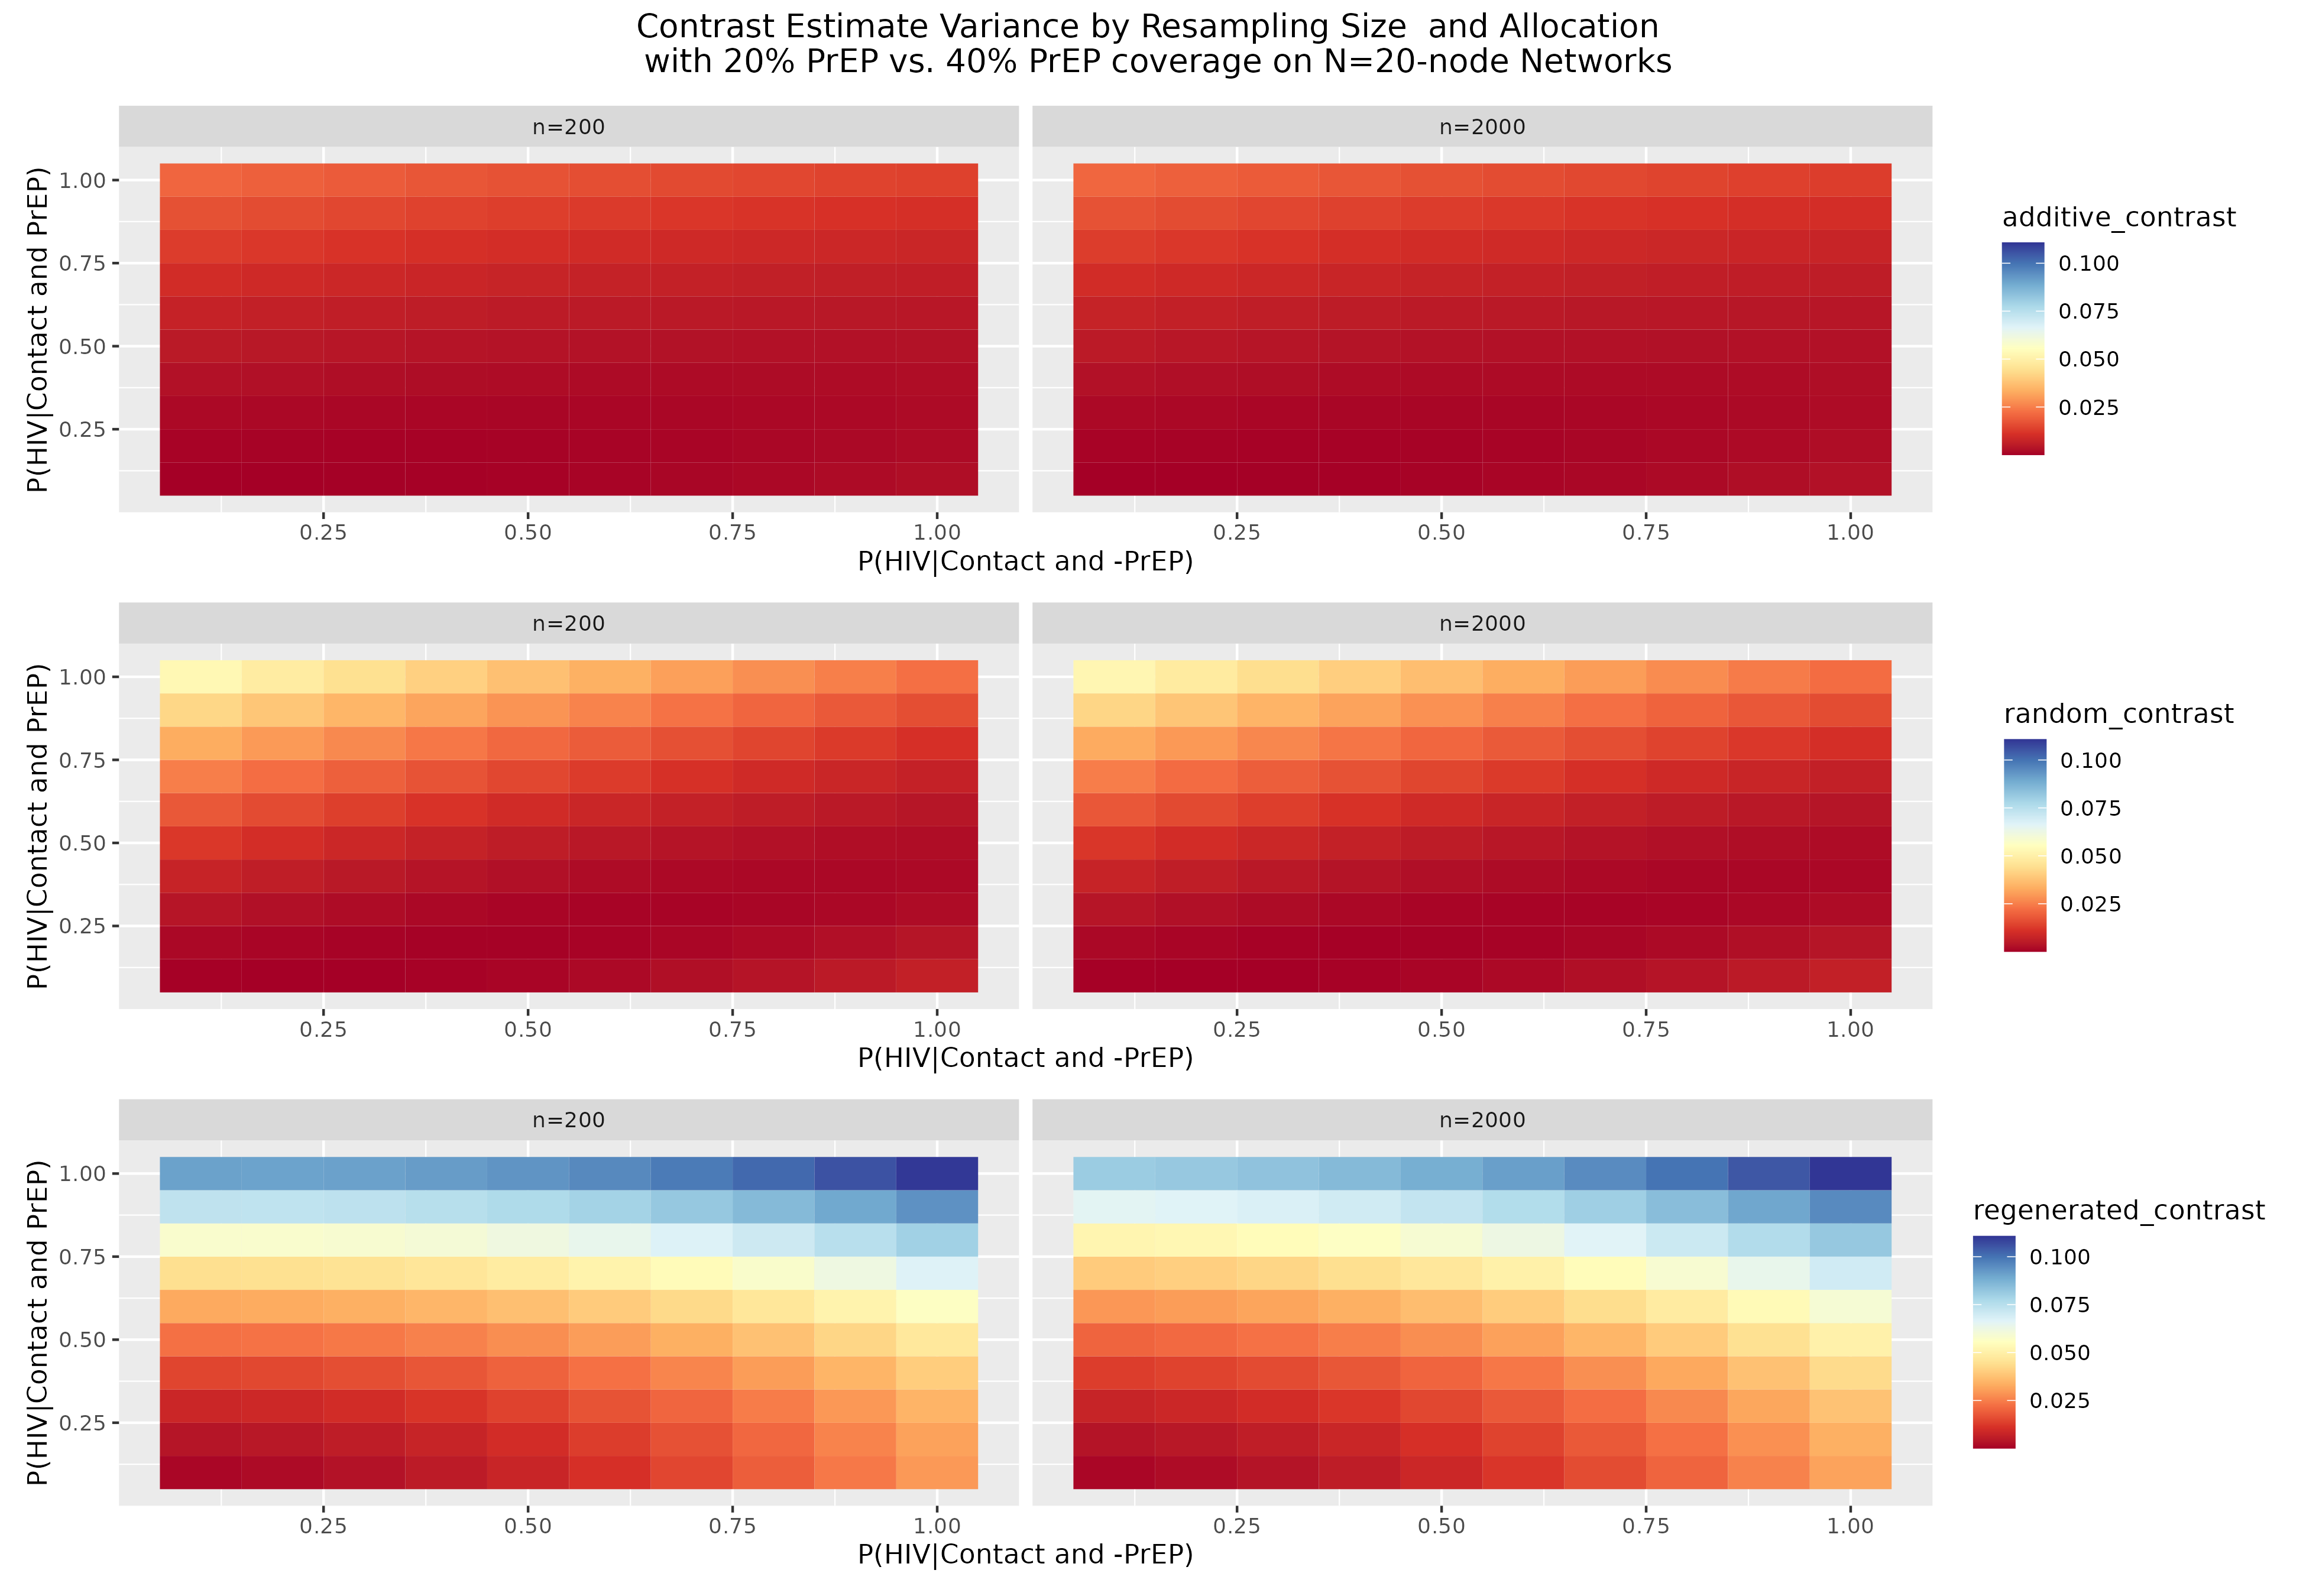
\includegraphics[width=\linewidth]{Corrected Figures/Resampling Size Variance Plot.png}
    \caption{Variance of Causal Contrast estimates as $\mathbb{P}\left[\text{HIV} \vert \neg \text{PrEP} \cap \text{Contact}\right]$ and $\mathbb{P}\left[\text{HIV} \vert \text{PrEP} \cap \text{Contact}\right]$ increase, stratified by resampling sample size. From top to bottom: ``additive" Variance of Contrast of random 20\% additional vs. random 20\% PrEP allocation control, ``random" Variance of Contrast of random 40\% PrEP allocation vs. random 20\% control, ``regenerated" Variance of Contrast of random 40\% allocation on regenerated network vs. random 20\% control.}
    \label{ffig:Figure S4.4}
\end{figure}
Much like with network size, effect modification of the relationship between underlying HIV risks and treatment strategy by resampling size is apparent in both the Mean and Variance plots above. We can see clearly from these plots that Contrast estimate variances differ not only in the range of magnitudes but also follow very different gradients under different treatment strategies.
\subsubsection{Effect Modification by HIV Prevalence}
\begin{figure}[H]
    \centering
    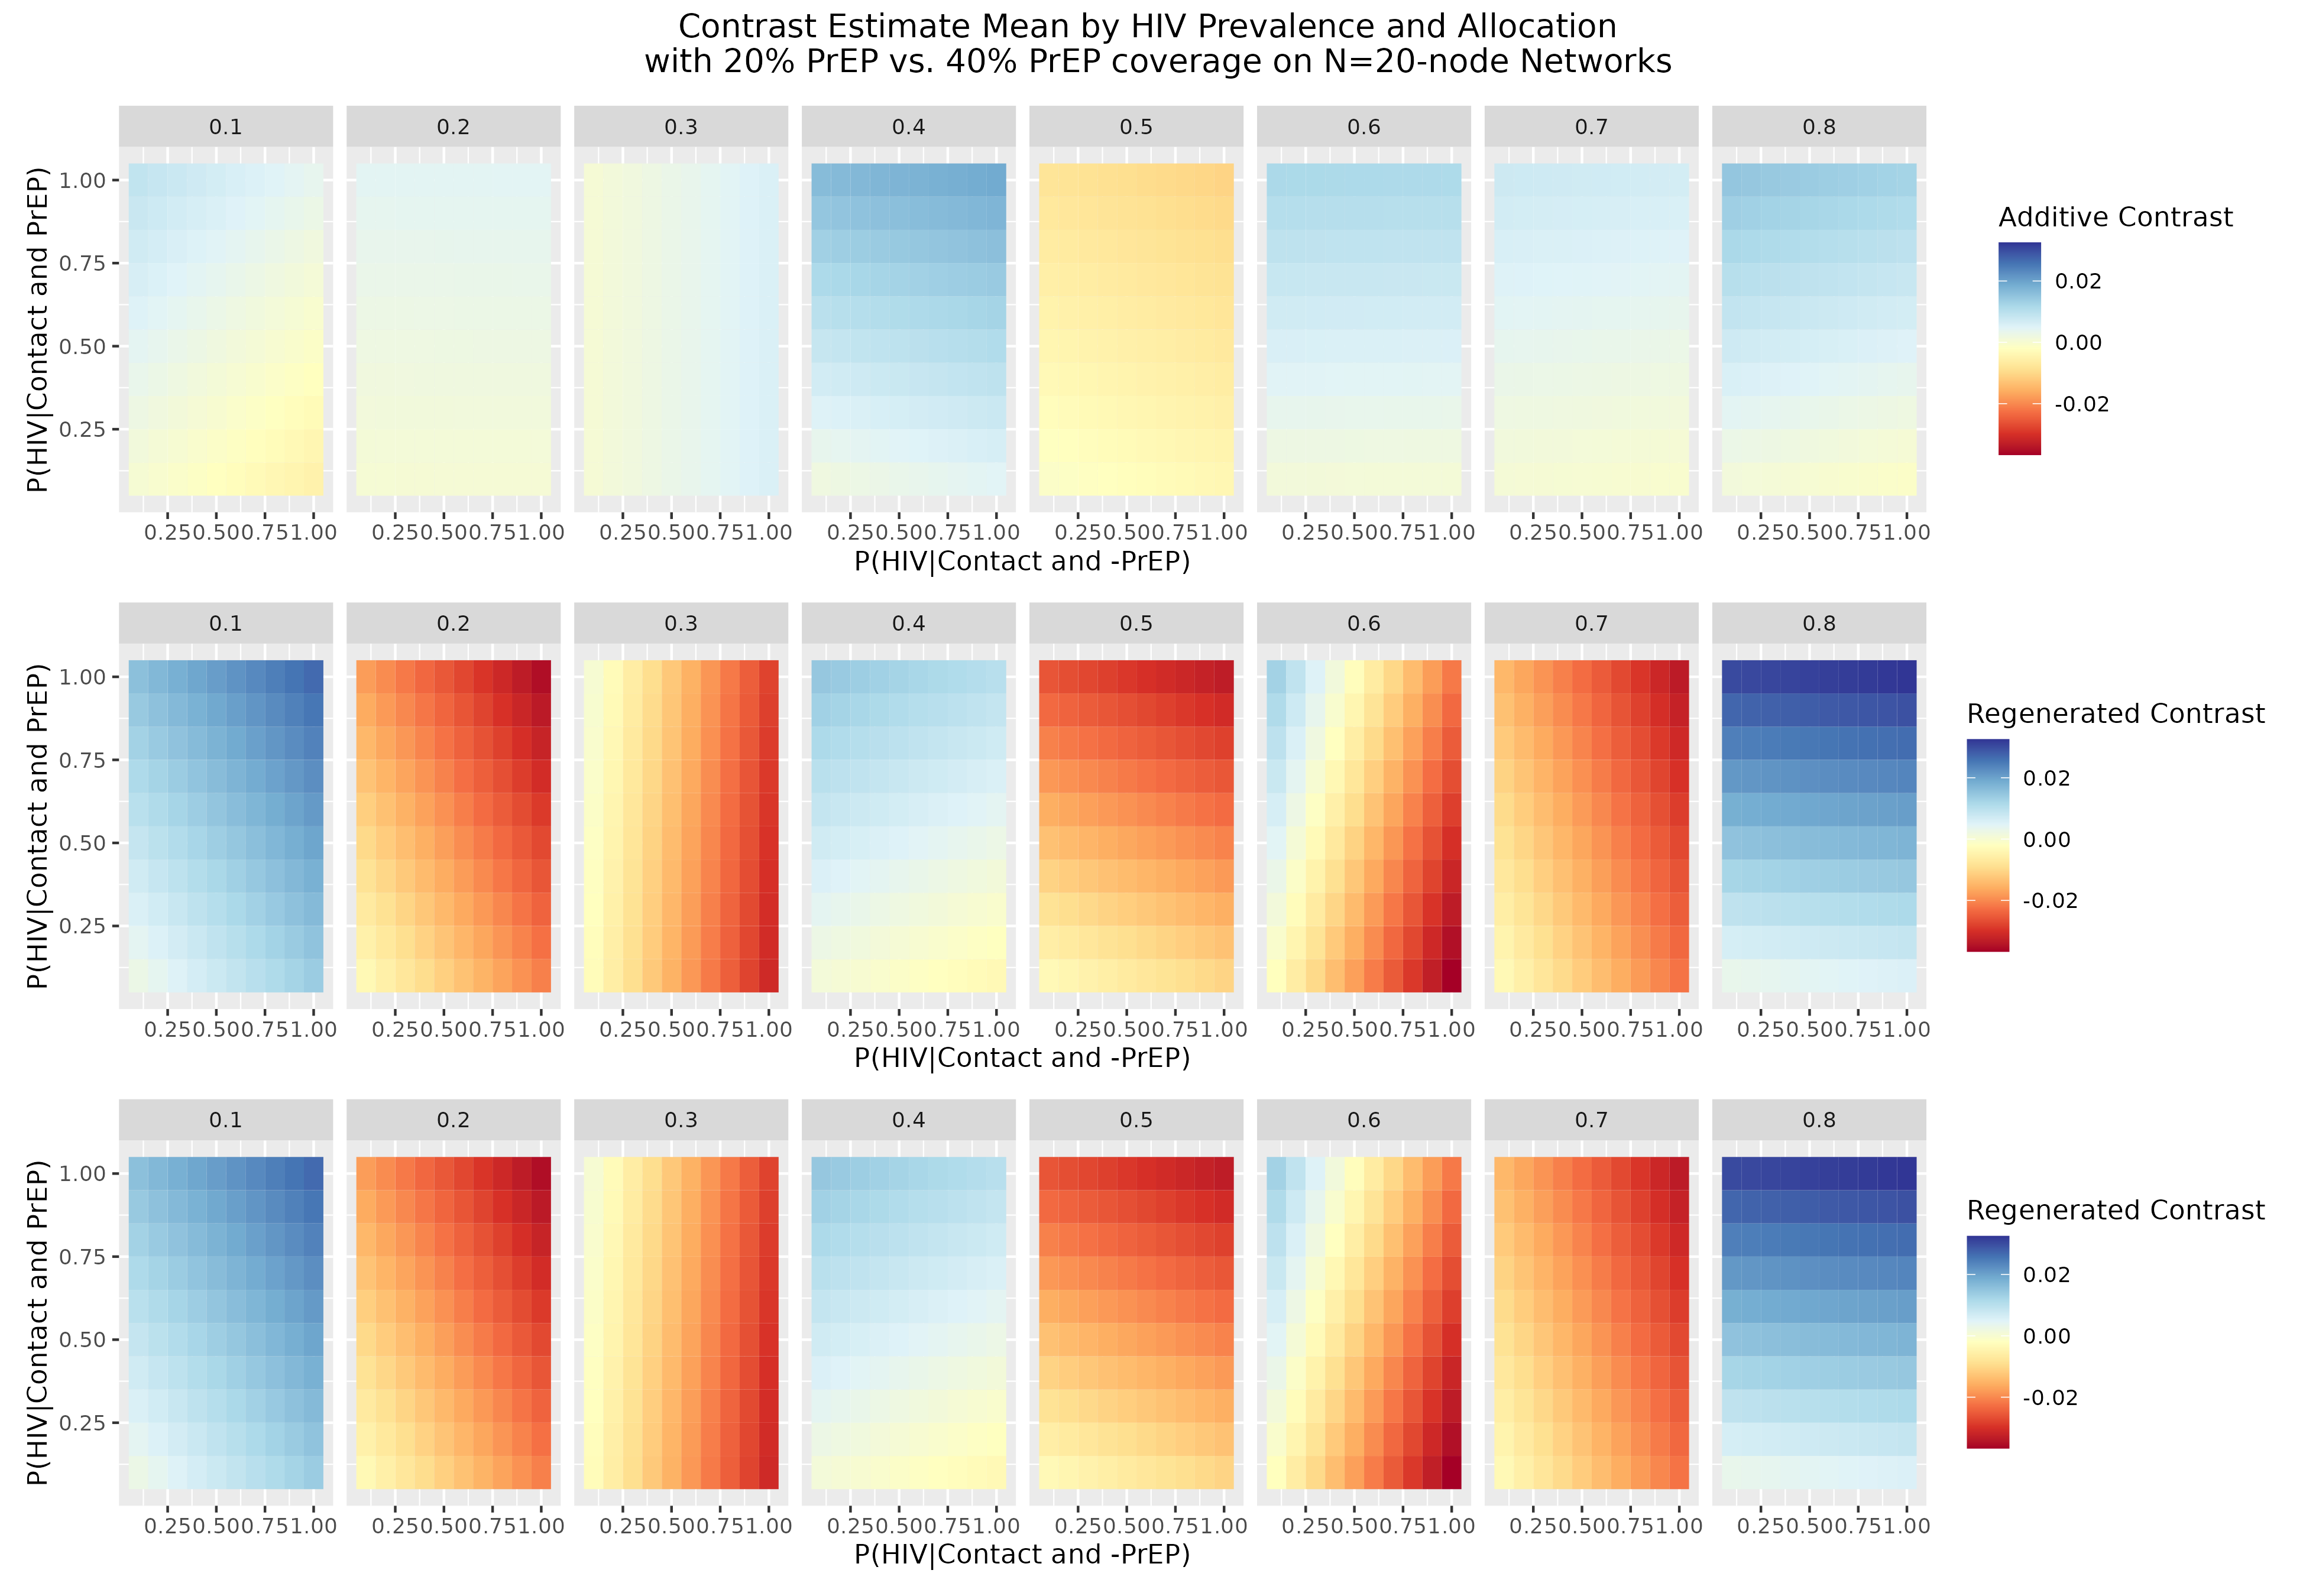
\includegraphics[width=\linewidth]{Corrected Figures/HIV Prevalence Mean Plot.png }
    \caption{Mean Causal Contrast estimates as $\mathbb{P}\left[\text{HIV} \vert \neg \text{PrEP} \cap \text{Contact}\right]$ and $\mathbb{P}\left[\text{HIV} \vert \text{PrEP} \cap \text{Contact}\right]$ increase,  stratified by HIV Prevalence. From top to bottom: ``additive" Mean Contrast of random 20\% additional vs. random 20\% PrEP allocation control, ``random" Mean Contrast of random 40\% PrEP allocation vs. random 20\% control, ``regenerated" Mean Contrast of random 40\% allocation on regenerated network vs. random 20\% control.}
    \label{fig:Figure S4.5}
\end{figure}
\begin{figure}[H]
    \centering
    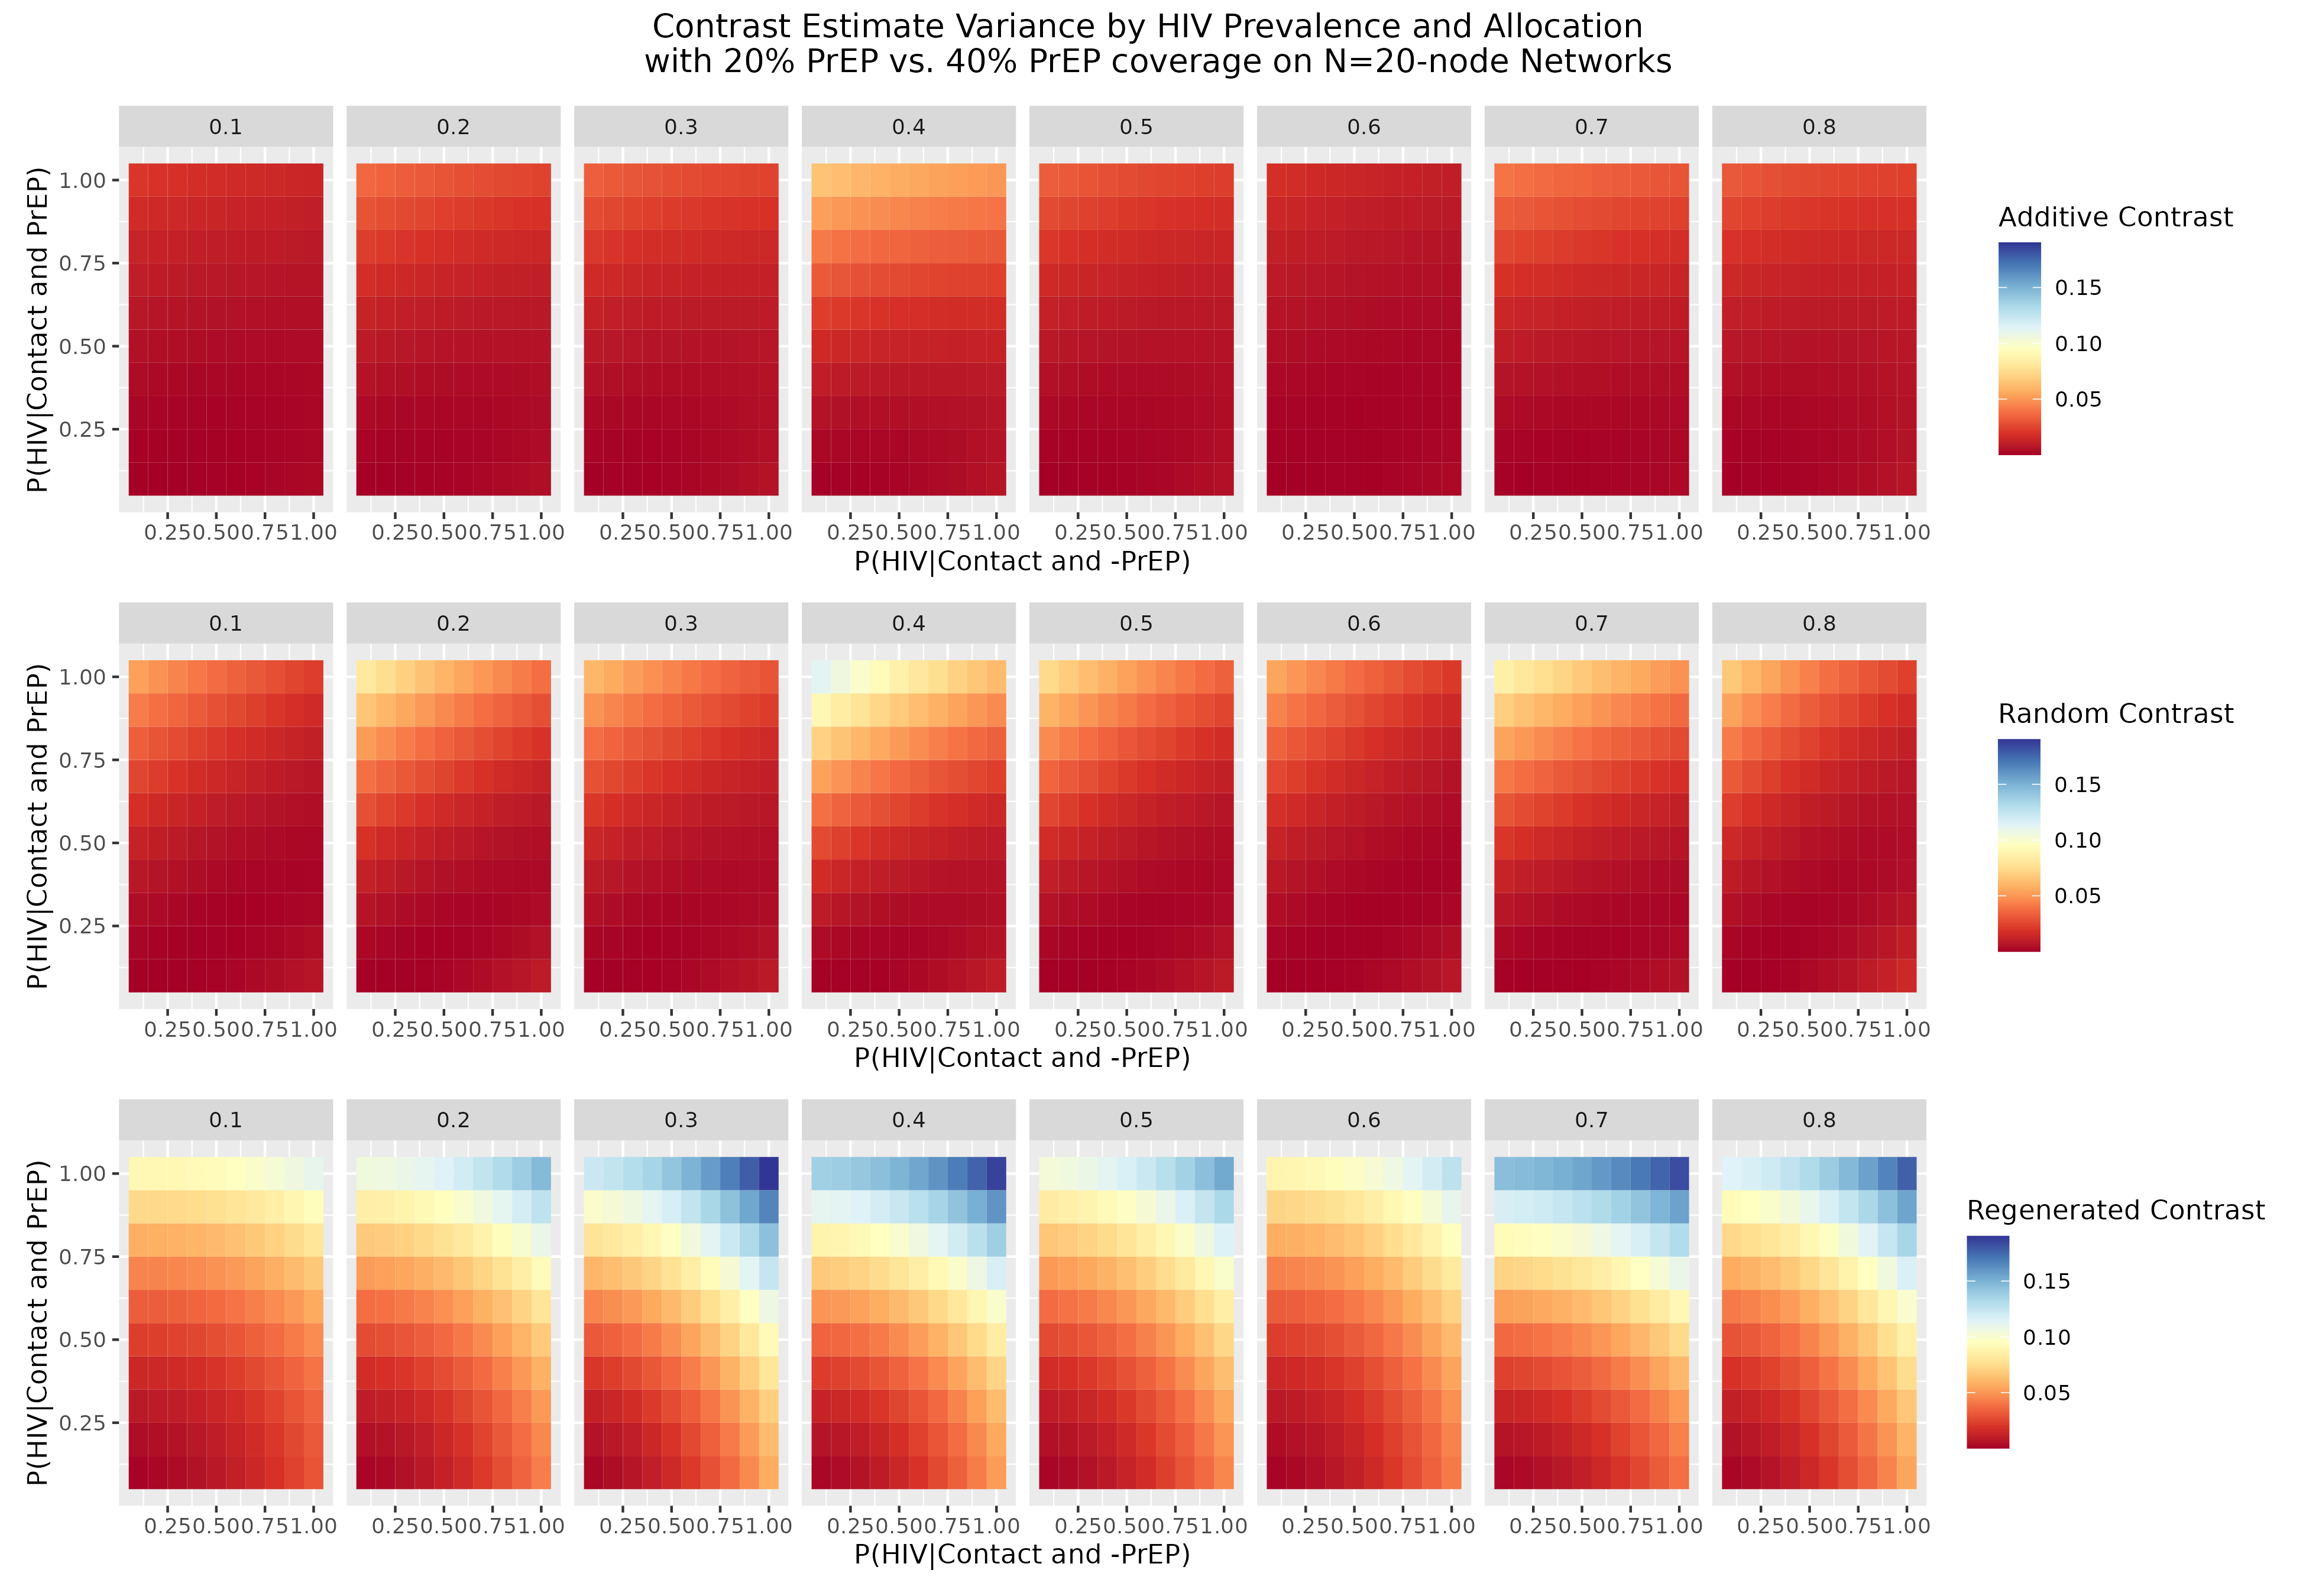
\includegraphics[width=\linewidth]{Corrected Figures/HIV Prevalence Variance Plot.png}
    \caption{Variance of Causal Contrast estimates as $\mathbb{P}\left[\text{HIV} \vert \neg \text{PrEP} \cap \text{Contact}\right]$ and $\mathbb{P}\left[\text{HIV} \vert \text{PrEP} \cap \text{Contact}\right]$ increase,  stratified by HIV Prevalence. From top to bottom: ``additive" Variance of Contrast of random 20\% additional vs. random 20\% PrEP allocation control, ``random" Variance of Contrast of random 40\% PrEP allocation vs. random 20\% control, ``regenerated" Variance of Contrast of random 40\% allocation on regenerated network vs. random 20\% control.}
    \label{fig:Figure S4.6}
\end{figure}

While it may be more obvious from the Variance plots in Figure \ref{fig:Figure S4.6} than in the Mean plots \ref{fig:Figure S4.5}, there is an apparent effect modification of the relationship between underlying HIV risks and treatment strategy by the initial HIV prevalence. We can see three distinct gradients in the magnitude of the contrast estimate Variance over the HIV risks for each of the treatment strategies, with distinct changes in these gradients by HIV prevalence. 
\subsubsection{Effect Modification by \texorpdfstring{$\mathbb{P}[\text{HIV } | \text {Contact } \cap \neg \text{ PrEP}]$}{ℙ[HIV | ¬PrEP]}}
\begin{figure}[H]
    \centering
    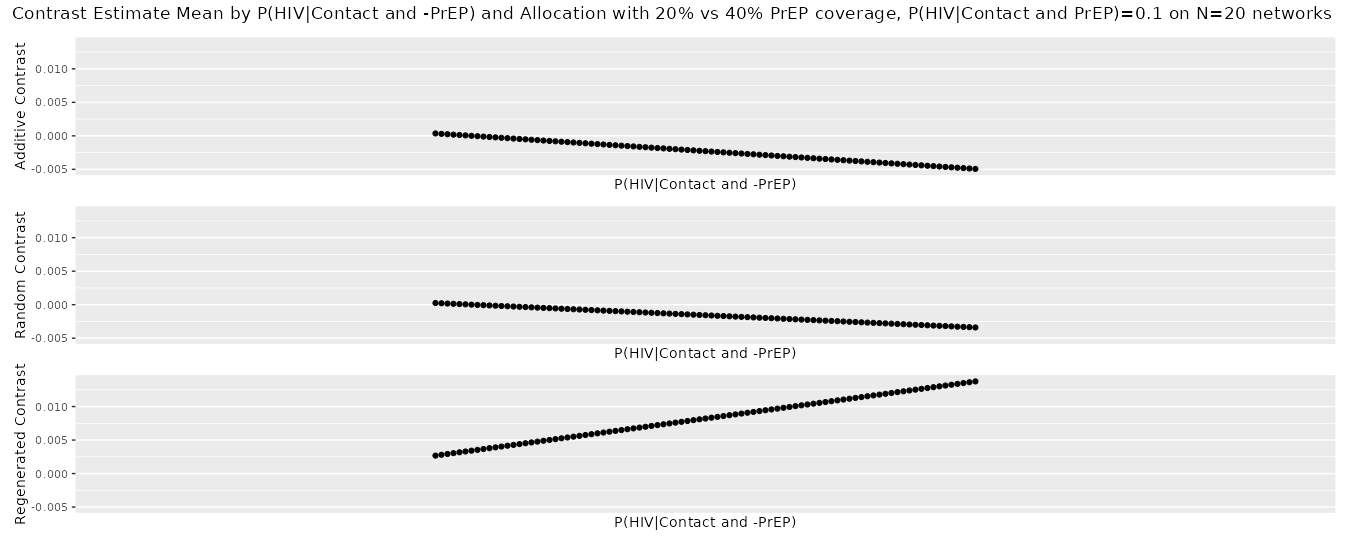
\includegraphics[width=\linewidth]{Corrected Figures/p1 Mean plots.png}
    \caption{Mean Causal Contrast estimates as $\mathbb{P}\left[\text{HIV } \vert \text {Contact } \cap \neg \text{ PrEP}\right]$ increases . From top to bottom: ``additive" Mean Contrast of random 20\% additional vs. random 20\% PrEP allocation control, ``random" Mean Contrast of random 40\% PrEP allocation vs. random 20\% control, ``regenerated" Mean Contrast of random 40\% allocation on regenerated network vs. random 20\% control.}
    \label{fig:Figure S4.7}
\end{figure}
\begin{figure}[H]
    \centering
    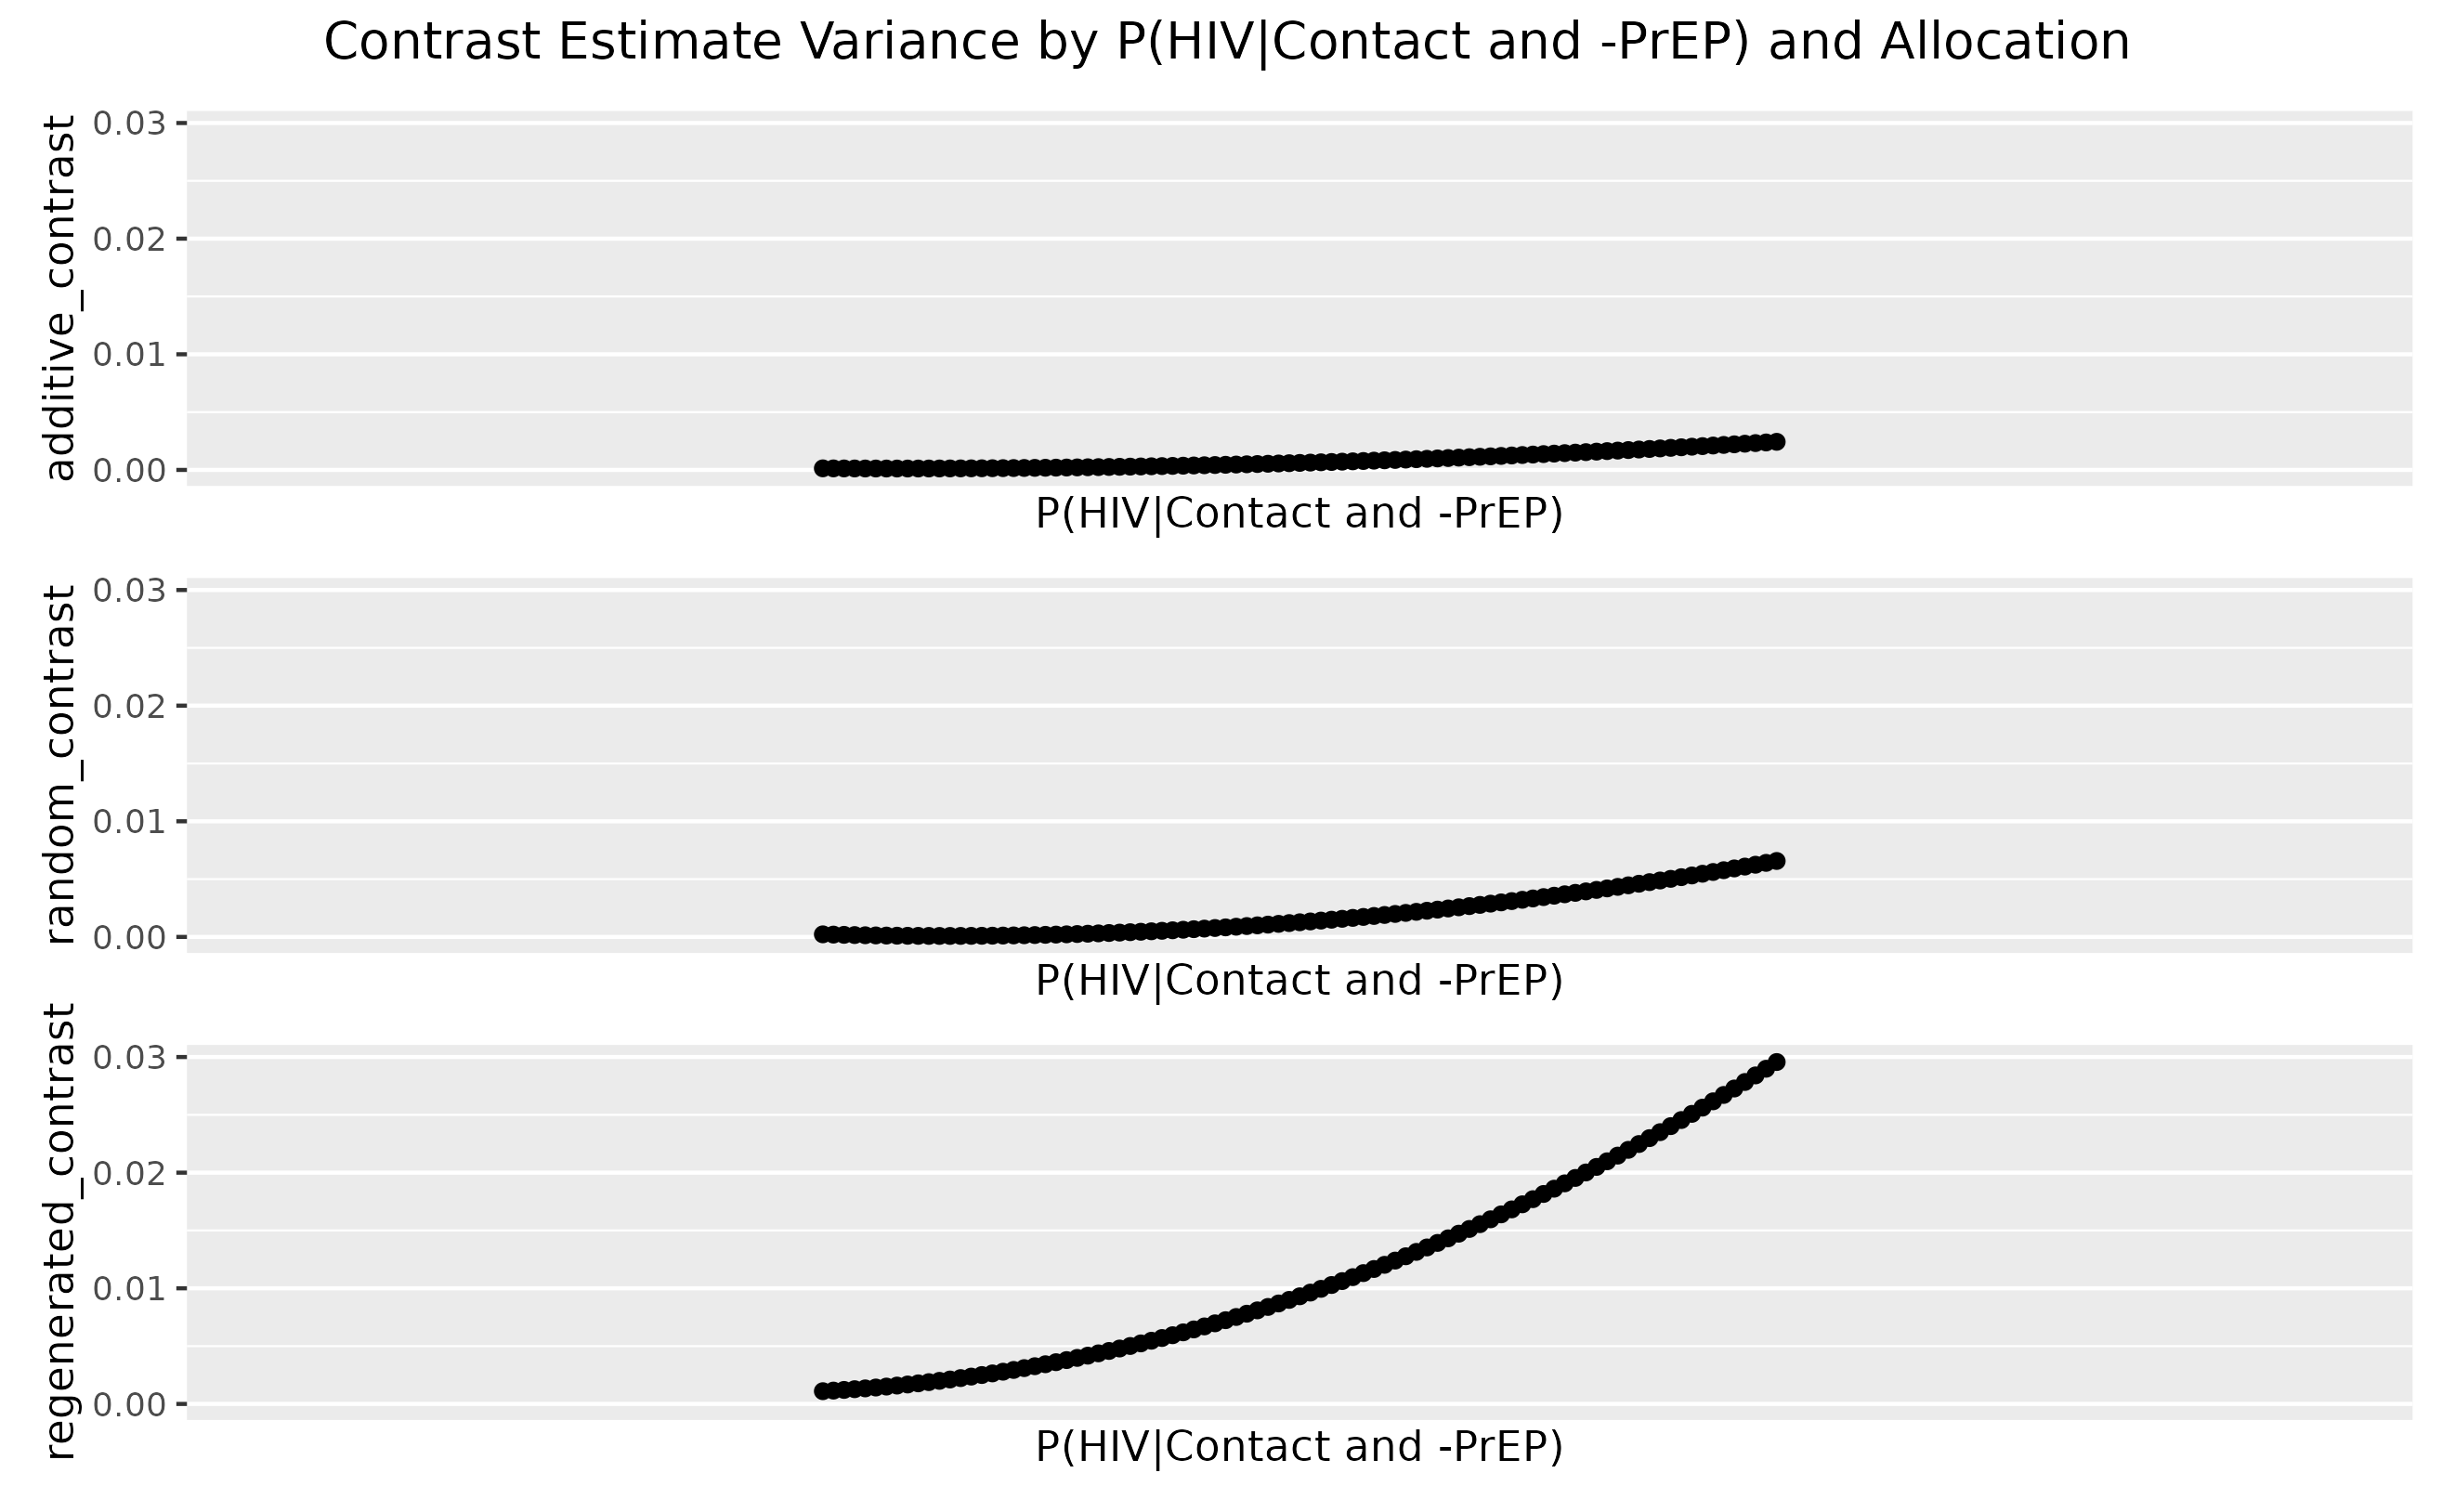
\includegraphics[width=\linewidth]{Corrected Figures/p1 Variance plots.png}
    \caption{Variance of Causal Contrast estimates as $\mathbb{P}\left[\text{HIV } \vert \text {Contact } \cap \neg \text{ PrEP}\right]$ increases .  From top to bottom: ``additive" Variance of Contrast of random 20\% additional vs. random 20\% PrEP allocation control, ``random" Variance of Contrast of random 40\% PrEP allocation vs. random 20\% control, ``regenerated" Variance of Contrast of random 40\% allocation on regenerated network vs. random 20\% control.}
    \label{fig:Figure S4.8}
\end{figure}
From the contrast estimate Mean and Variance plots in figures \ref{fig:Figure S4.7} and \ref{fig:Figure S4.8} above, we observe the effect modification of the relationship between the underlying risk of HIV given contact and no treatment and HIV risk by treatment strategy. Whilst in the ``additive" treatment strategy, the contrast estimate Mean and Variance are both very small and relatively constant except for relatively large values of $\mathbb{P}\left[\text{HIV } \vert \text {Contact } \cap \neg \text{ PrEP}\right]$. The ``random" and ``regenerated" treatment strategies show marked heteroskedasticity beginning with much smaller values of $\mathbb{P}\left[\text{HIV } \vert \text {Contact } \cap \neg \text{ PrEP}\right]$, with the "regenerated" strategy usually having larger variability than the ``random" strategy for the same value of $\mathbb{P}\left[\text{HIV } \vert \text {Contact } \cap \neg \text{ PrEP}\right]$.  
\subsubsection{Effect Modification by \texorpdfstring{$\mathbb{P}\left[\text{HIV } \vert \text {Contact } \cap \text{ PrEP}\right]$}{ℙ[HIV | PrEP]}}
\begin{figure}[H]
    \centering
    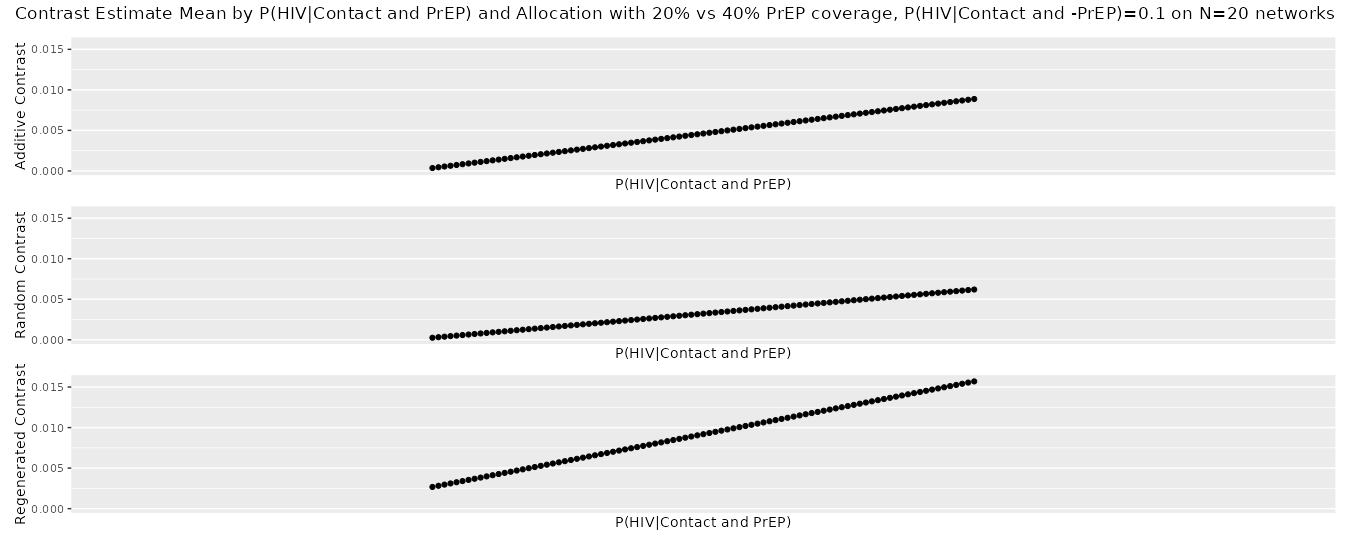
\includegraphics[width=\linewidth]{Corrected Figures/p2 Mean plots.png}
    \caption{Mean Causal Contrast estimates as $\mathbb{P}\left[\text{HIV } \vert \text{ PrEP}\right]$ increases . From top to bottom: ``additive" Mean Contrast of random 20\% additional vs. random 20\% PrEP allocation control, ``random" Mean Contrast of random 40\% PrEP allocation vs. random 20\% control, ``regenerated" Mean Contrast of random 40\% allocation on regenerated network vs. random 20\% control.}
    \label{fig:Figure S4.9}

\end{figure}

\begin{figure}[H]
    \centering
    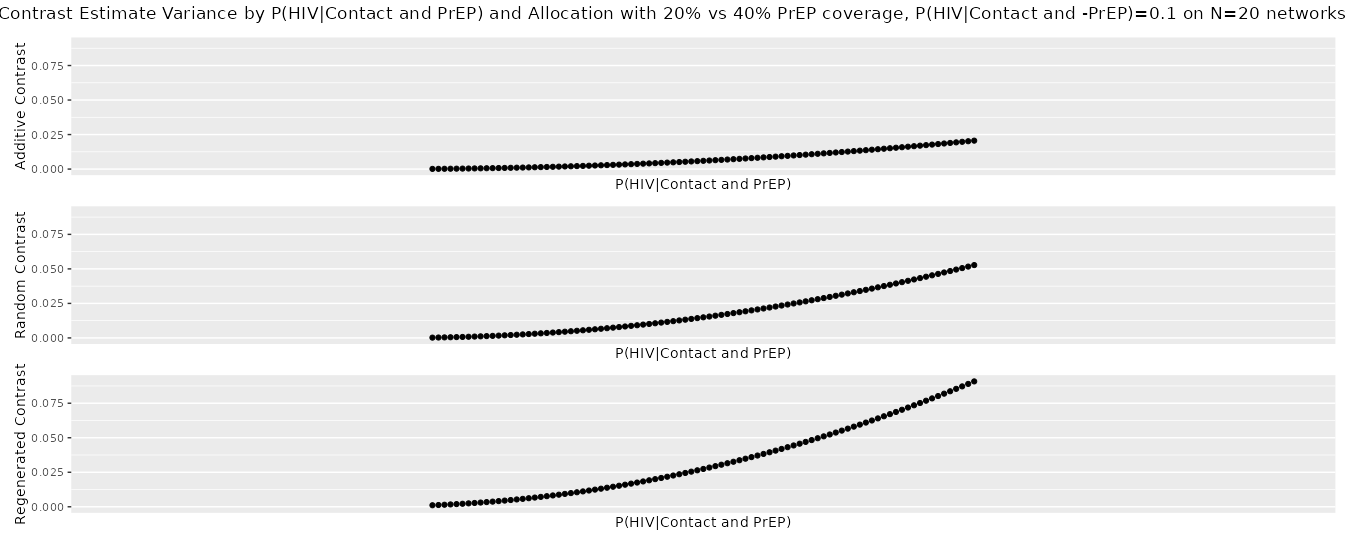
\includegraphics[width=\linewidth]{Corrected Figures/p2 Variance plots.png}
    \caption{Variance of Causal Contrast estimates as $\mathbb{P}\left[\text{HIV } \vert \text{ PrEP}\right]$ increases .  From top to bottom: ``additive" Variance of Contrast of random 20\% additional vs. random 20\% PrEP allocation control, ``random" Variance of Contrast of random 40\% PrEP allocation vs. random 20\% control, ``regenerated" Variance of Contrast of random 40\% allocation on regenerated network vs. random 20\% control.}
    \label{fig:Figure S4.10}
\end{figure}
Much like with the underlying risk of HIV given no treatment, we observe effect modification of the relationship between the underlying risk of HIV given infectious contact and PrEP treatment by allocation strategy. This modification is apparent in both Causal Contrast estimate Mean and Variance plots in Figure \ref{fig:Figure S4.9} and \ref{fig:Figure S4.10}, respectively. While the modification is qualitatively similar to that for the no-treatment risk, it is interesting to note that the range of both Mean and Variance magnitudes is larger for $\mathbb{P}\left[\text{HIV } \vert \text{ PrEP}\right]$ than for $\mathbb{P}\left[\text{HIV } \vert \text {Contact } \cap \neg \text{ PrEP}\right]$.

\subsubsection{Varying PrEP contrasts in ER model}
\begin{figure}[H]
    \centering
    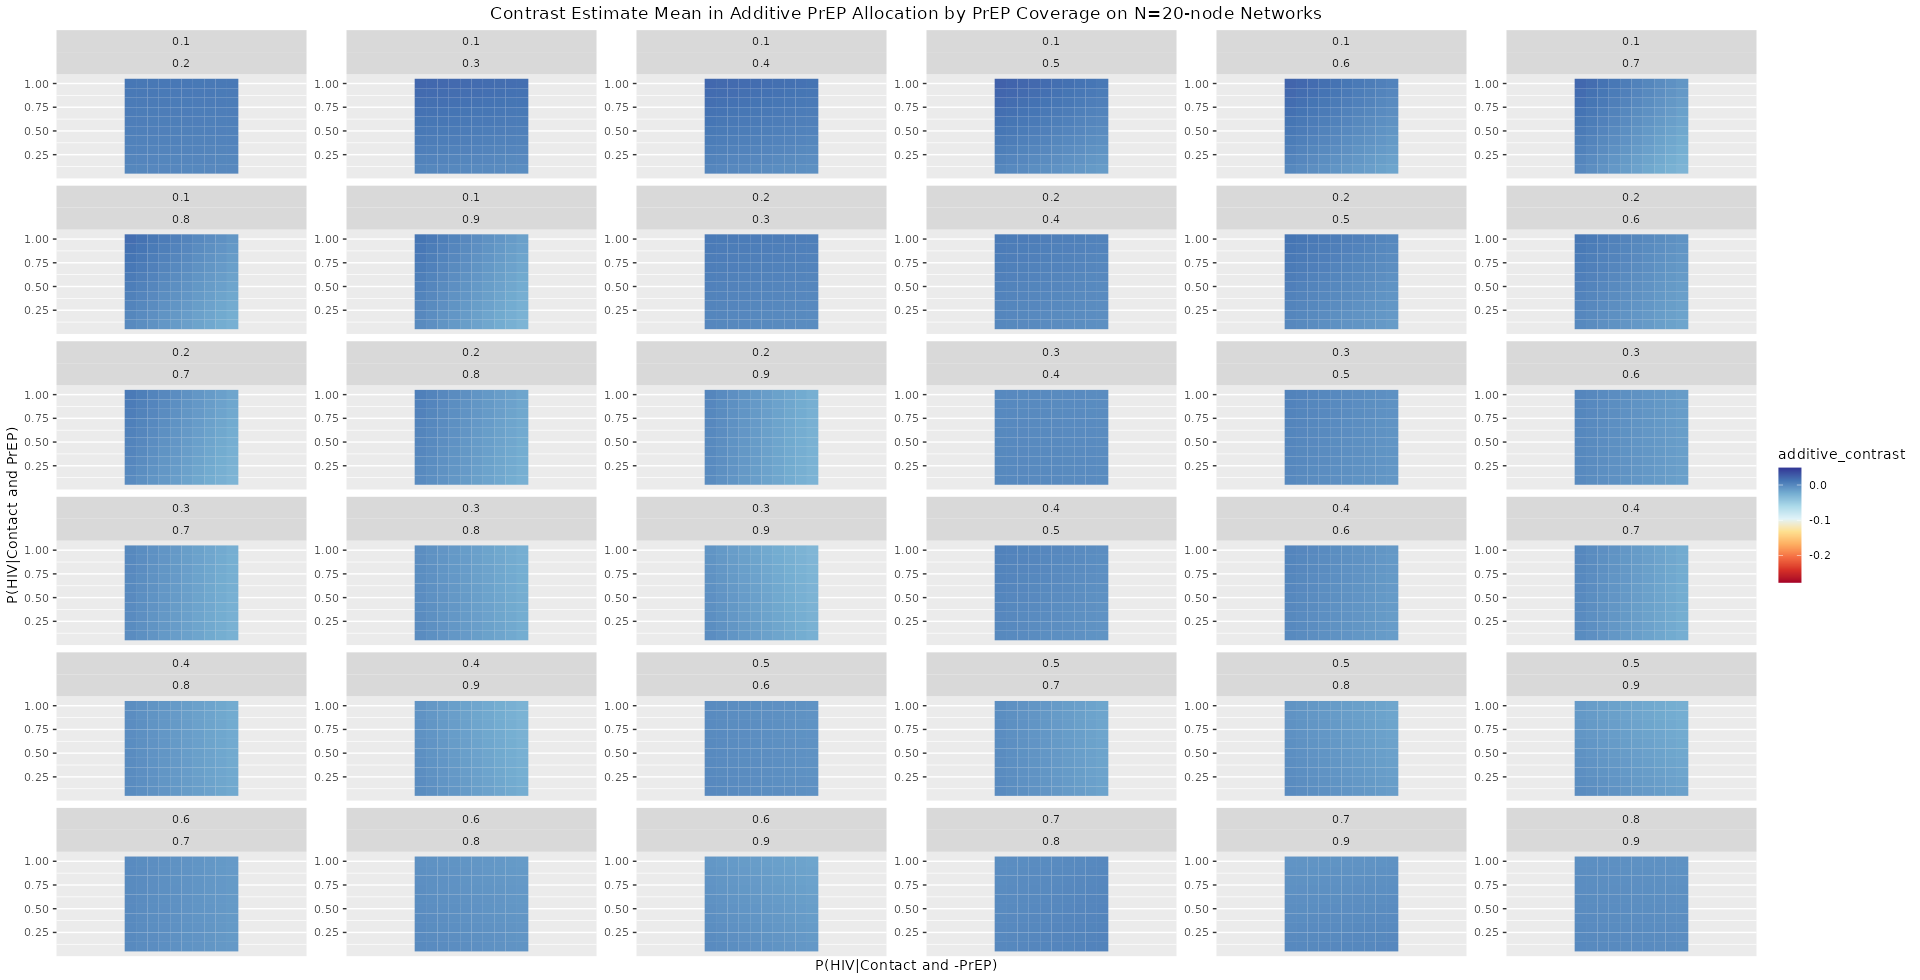
\includegraphics[width=\linewidth]{Corrected Figures/PrEP Additive Mean Plots.png}
    \caption{Mean Causal Contrast estimates as $\mathbb{P}\left[\text{HIV} \vert \neg \text{PrEP} \cap \text{Contact}\right]$ and $\mathbb{P}\left[\text{HIV} \vert \text{PrEP} \cap \text{Contact}\right]$ increase, stratified by random PrEP1\% additional vs. random PrEP2-PrEP1 \% PrEP allocation control. Top number indicates PrEP1 \% control coverage. Bottom number is PrEP2 counterfactual coverage. }
    \label{fig:Figure S4.11}
\end{figure}
\begin{figure}[H]
    \centering
    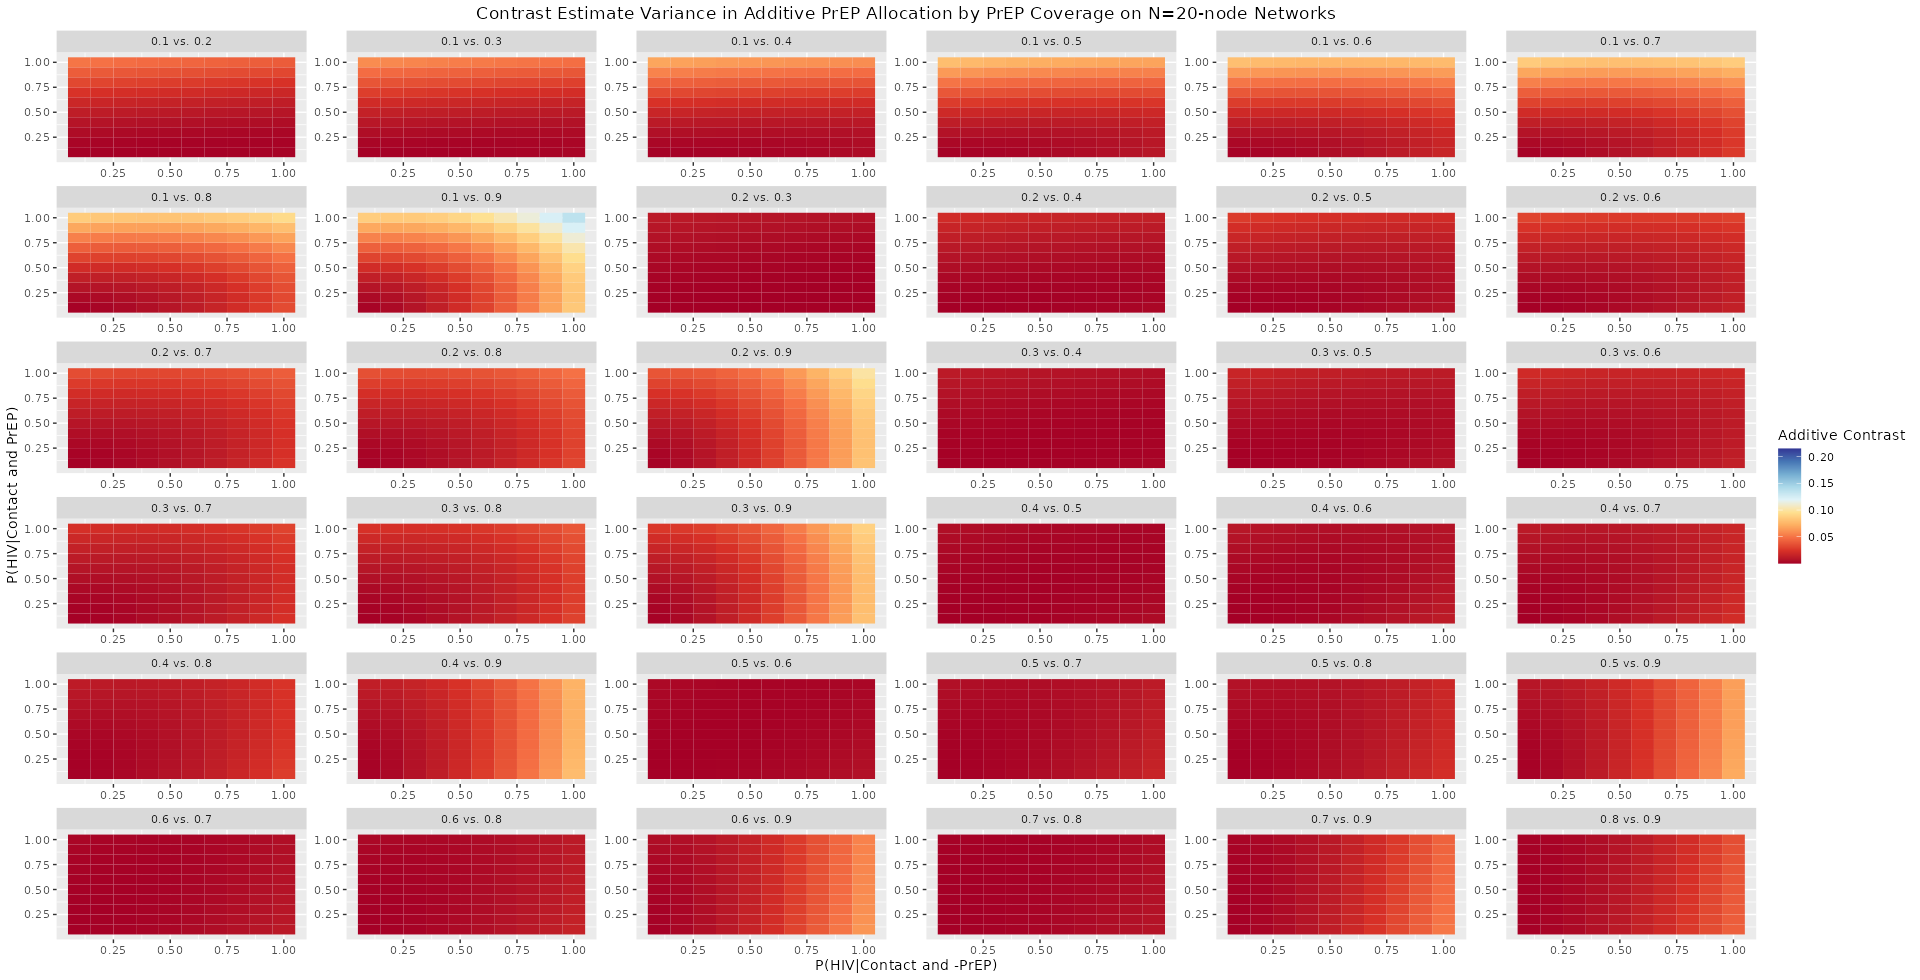
\includegraphics[width=\linewidth]{Corrected Figures/PrEP Additive Variance Plots.png}
    \caption{Variance of Causal Contrast estimates as $\mathbb{P}\left[\text{HIV} \vert \neg \text{PrEP} \cap \text{Contact}\right]$ and $\mathbb{P}\left[\text{HIV} \vert \text{PrEP} \cap \text{Contact}\right]$ increase, stratified by random PrEP2-PrEP1\% additional vs. random PrEP1 \% PrEP allocation control. Top number indicates PrEP1/control coverage. The bottom number is PrEP2 counterfactual coverage.}
    \label{fig:Figure S4.12}
\end{figure}
\begin{figure}[H]
    \centering
    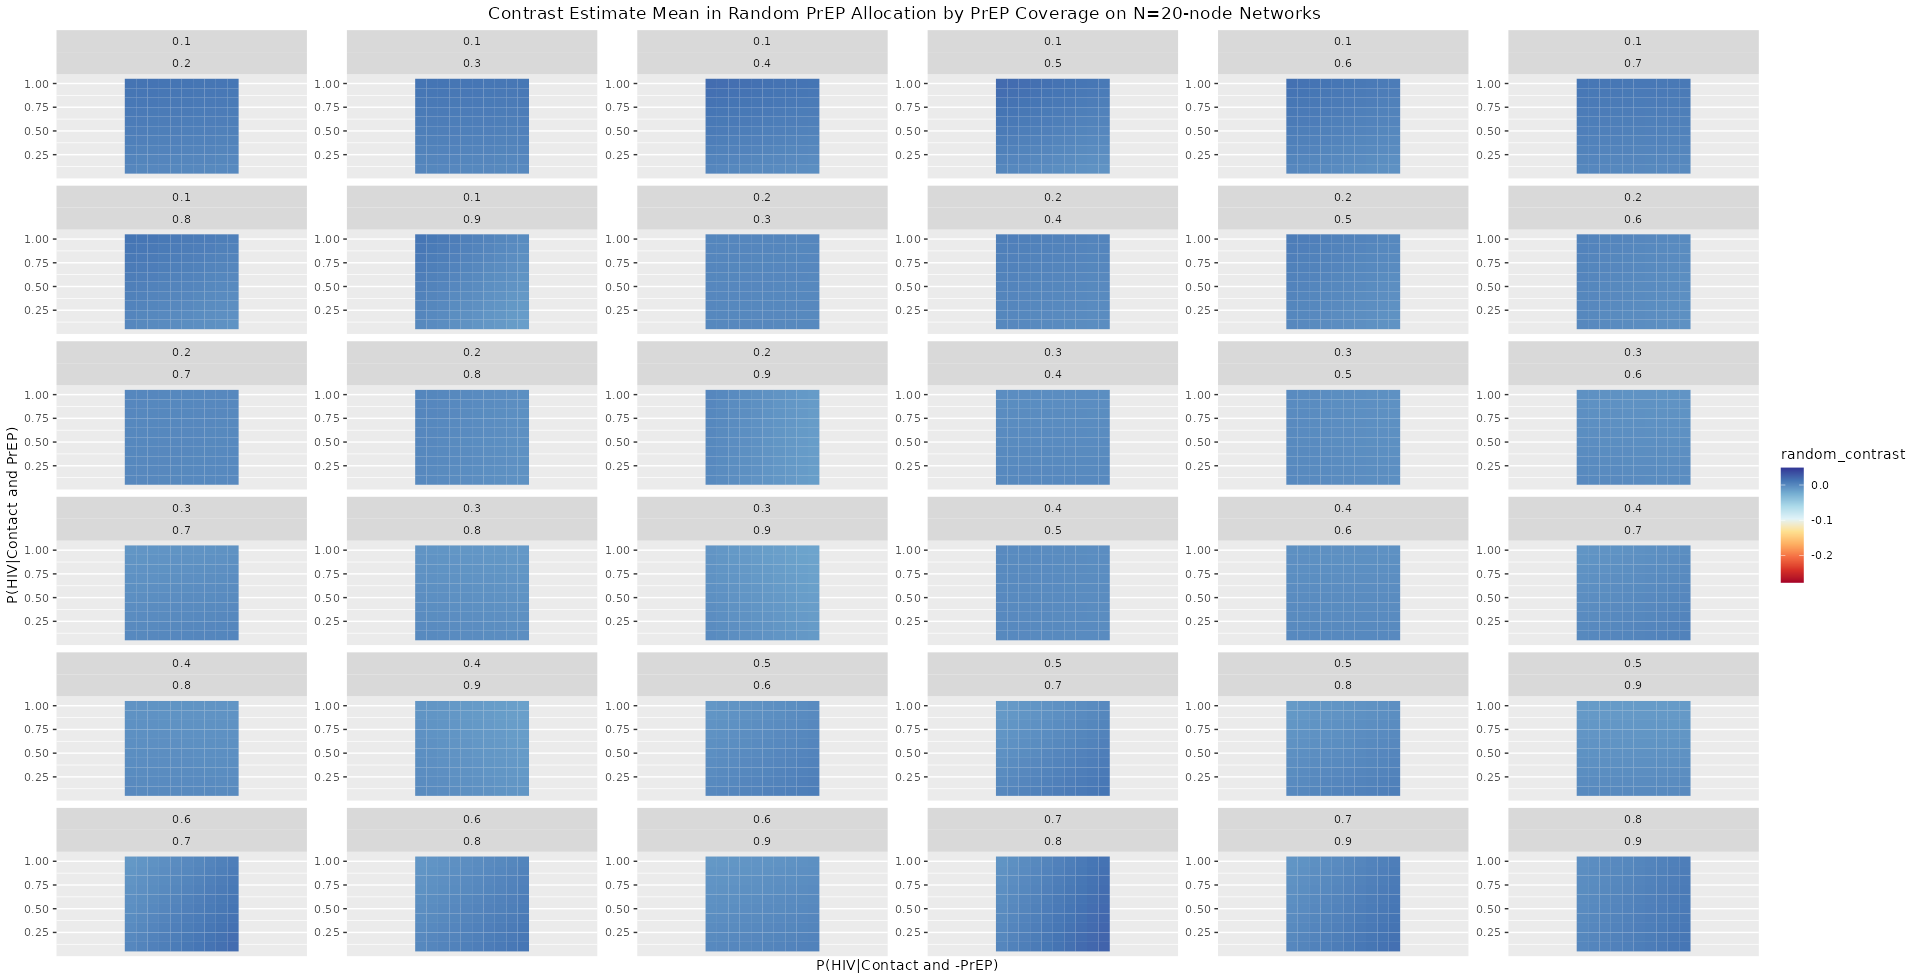
\includegraphics[width=\linewidth]{Corrected Figures/PrEP Random Mean Plots.png}
    \caption{Mean Causal Contrast estimates as $\mathbb{P}\left[\text{HIV} \vert \neg \text{PrEP} \cap \text{Contact}\right]$ and $\mathbb{P}\left[\text{HIV} \vert \text{PrEP} \cap \text{Contact}\right]$ increase, stratified by random PrEP2\% vs. random PrEP1\% PrEP allocation control. The top number indicates PrEP1/control coverage. The bottom number is PrEP2 counterfactual coverage.}
    \label{fig:Figure S4.13}
\end{figure}
\begin{figure}[H]
    \centering
    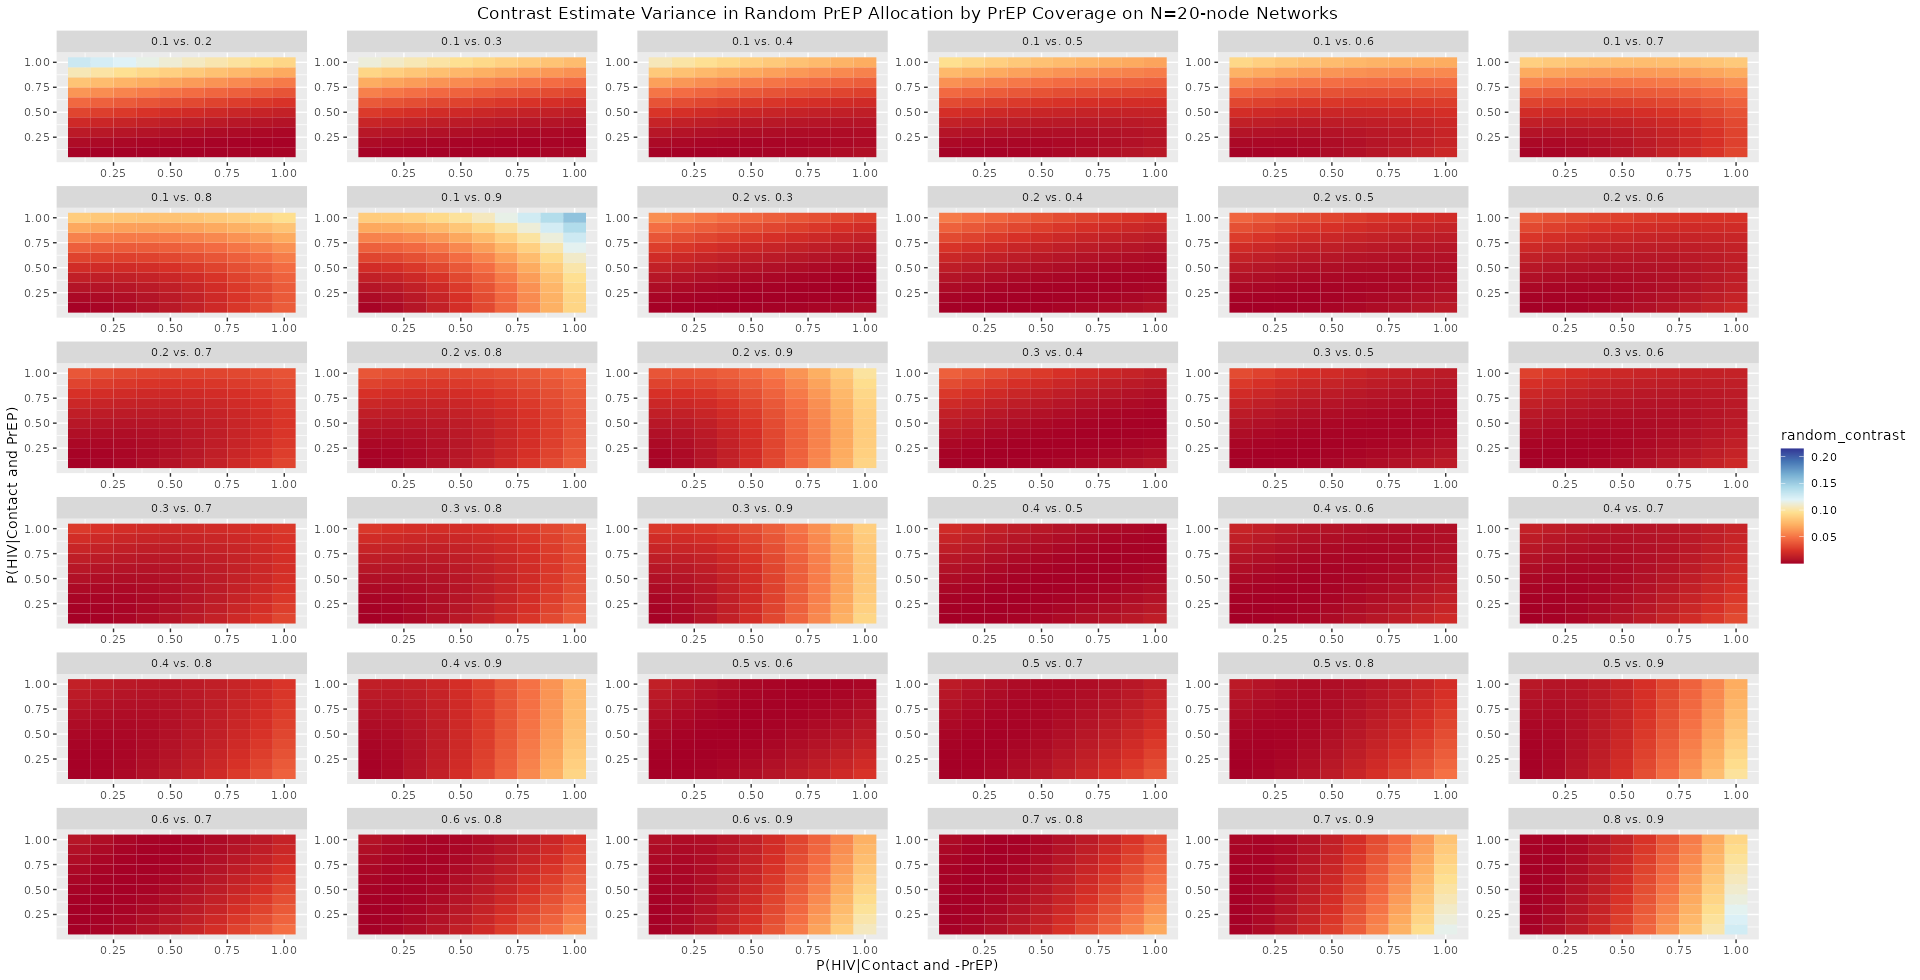
\includegraphics[width=\linewidth]{Corrected Figures/PrEP Random Variance Plots.png}
    \caption{Variance of Causal Contrast estimates as $\mathbb{P}\left[\text{HIV} \vert \neg \text{PrEP} \cap \text{Contact}\right]$ and $\mathbb{P}\left[\text{HIV} \vert \text{PrEP} \cap \text{Contact}\right]$ increase, stratified by random PrEP2\% vs. random PrEP1\% PrEP allocation control. The top number indicates PrEP1/control coverage. The bottom number is PrEP2 counterfactual coverage.}
    \label{fig:Figure S4.14}
\end{figure}
\begin{figure}[H]
    \centering
    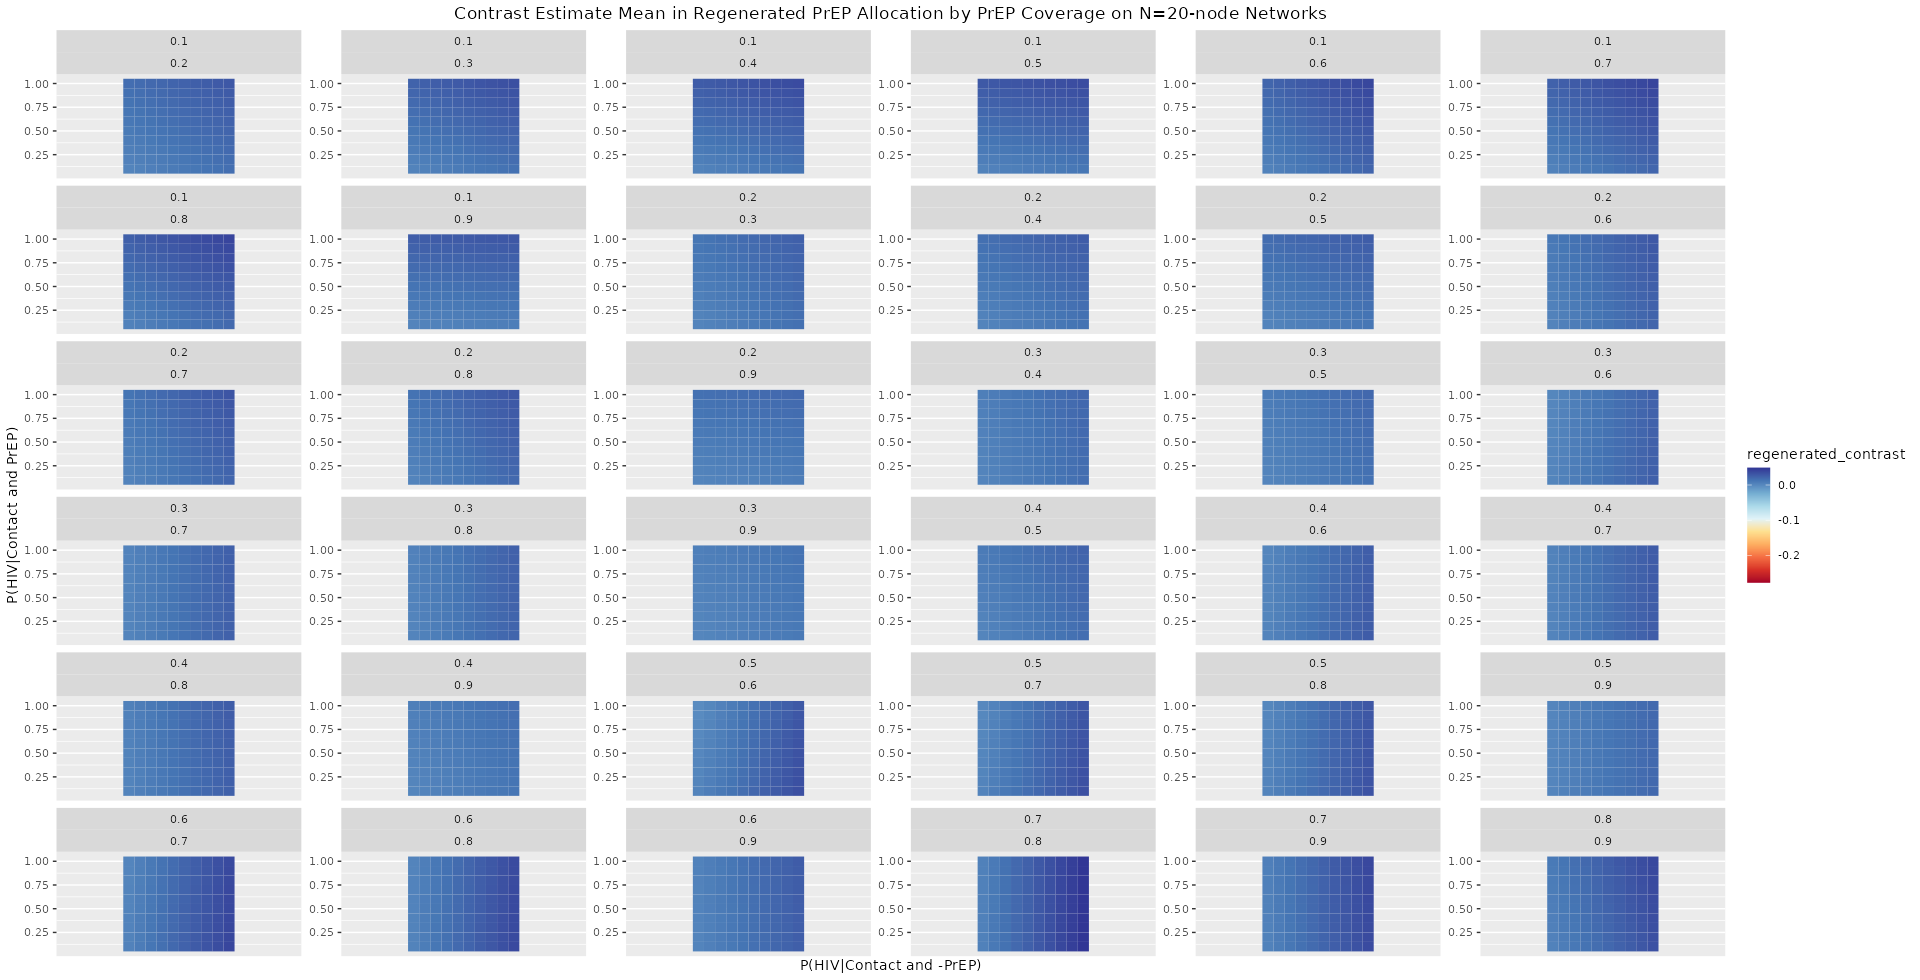
\includegraphics[width=\linewidth]{Corrected Figures/PrEP Regenerated Mean Plots.png}
    \caption{Mean of Causal Contrast estimates as $\mathbb{P}\left[\text{HIV} \vert \neg \text{PrEP} \cap \text{Contact}\right]$ and $\mathbb{P}\left[\text{HIV} \vert \text{PrEP} \cap \text{Contact}\right]$ increase, stratified by  random PrEP1 \% allocation vs random PrEP2\% allocation on a regenerated network. The top number indicates PrEP1/control coverage. The bottom number is PrEP2 counterfactual coverage.}
    \label{fig:Figure S4.15}
\end{figure}
\begin{figure}[H]
    \centering
    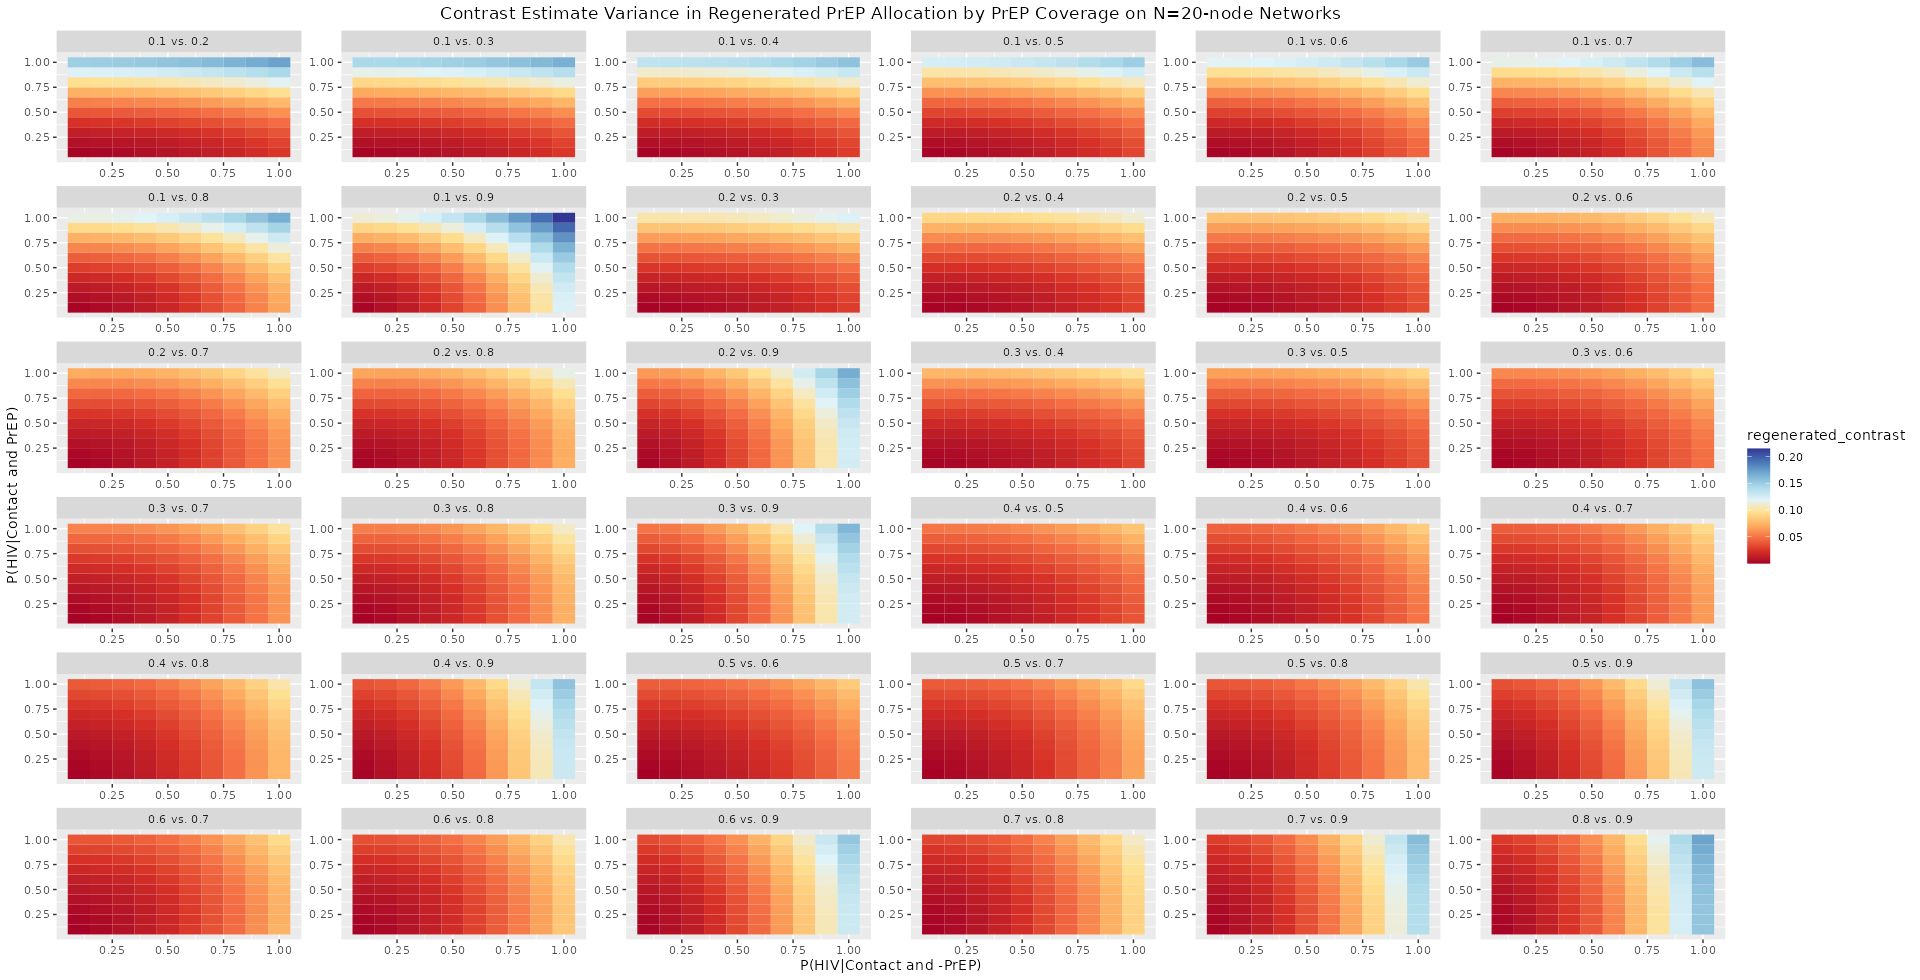
\includegraphics[width=\linewidth]{Corrected Figures/PrEP Regenerated Variance Plots.png}
    \caption{Variance of Causal Contrast estimates as $\mathbb{P}\left[\text{HIV} \vert \neg \text{PrEP} \cap \text{Contact}\right]$ and $\mathbb{P}\left[\text{HIV} \vert \text{PrEP} \cap \text{Contact}\right]$ increase, stratified by random PrEP1 \% allocation vs random PrEP2\% allocation on a regenerated network. The top number indicates PrEP1/control coverage. The bottom number is PrEP2 counterfactual coverage. }
    \label{fig:Figure S4.16}
\end{figure}

We can observe from the Causal Contrast Mean and Variance plots in Figures \ref{fig:Figure S4.11}-\ref{fig:Figure S4.16} that there is an effect modification of the relationship between underlying HIV risks and treatment strategy by the choices of PrEP treatment contrasts. This modification is easier to identify in the Variance plots, as once again the variances for the regenerated allocation strategy contrasts display a completely different gradient across underlying risks from the additive and random strategy for all pairs of PrEP coverages. While the gradients are more similar between the random and additive strategies, there are still clear differences in contrast Variance magnitude for given choices of PrEP coverage and HIV risks. With respect to the contrast estimate Mean, effect modification is more subtle between the random and additive strategies and more apparent when comparing these two to the regenerated strategy contrasts. 
\subsection{Other Network Models}

\subsubsection{Effect Modification by Network Generating Model with Default Parameters}
\begin{figure}[H]
    \centering
    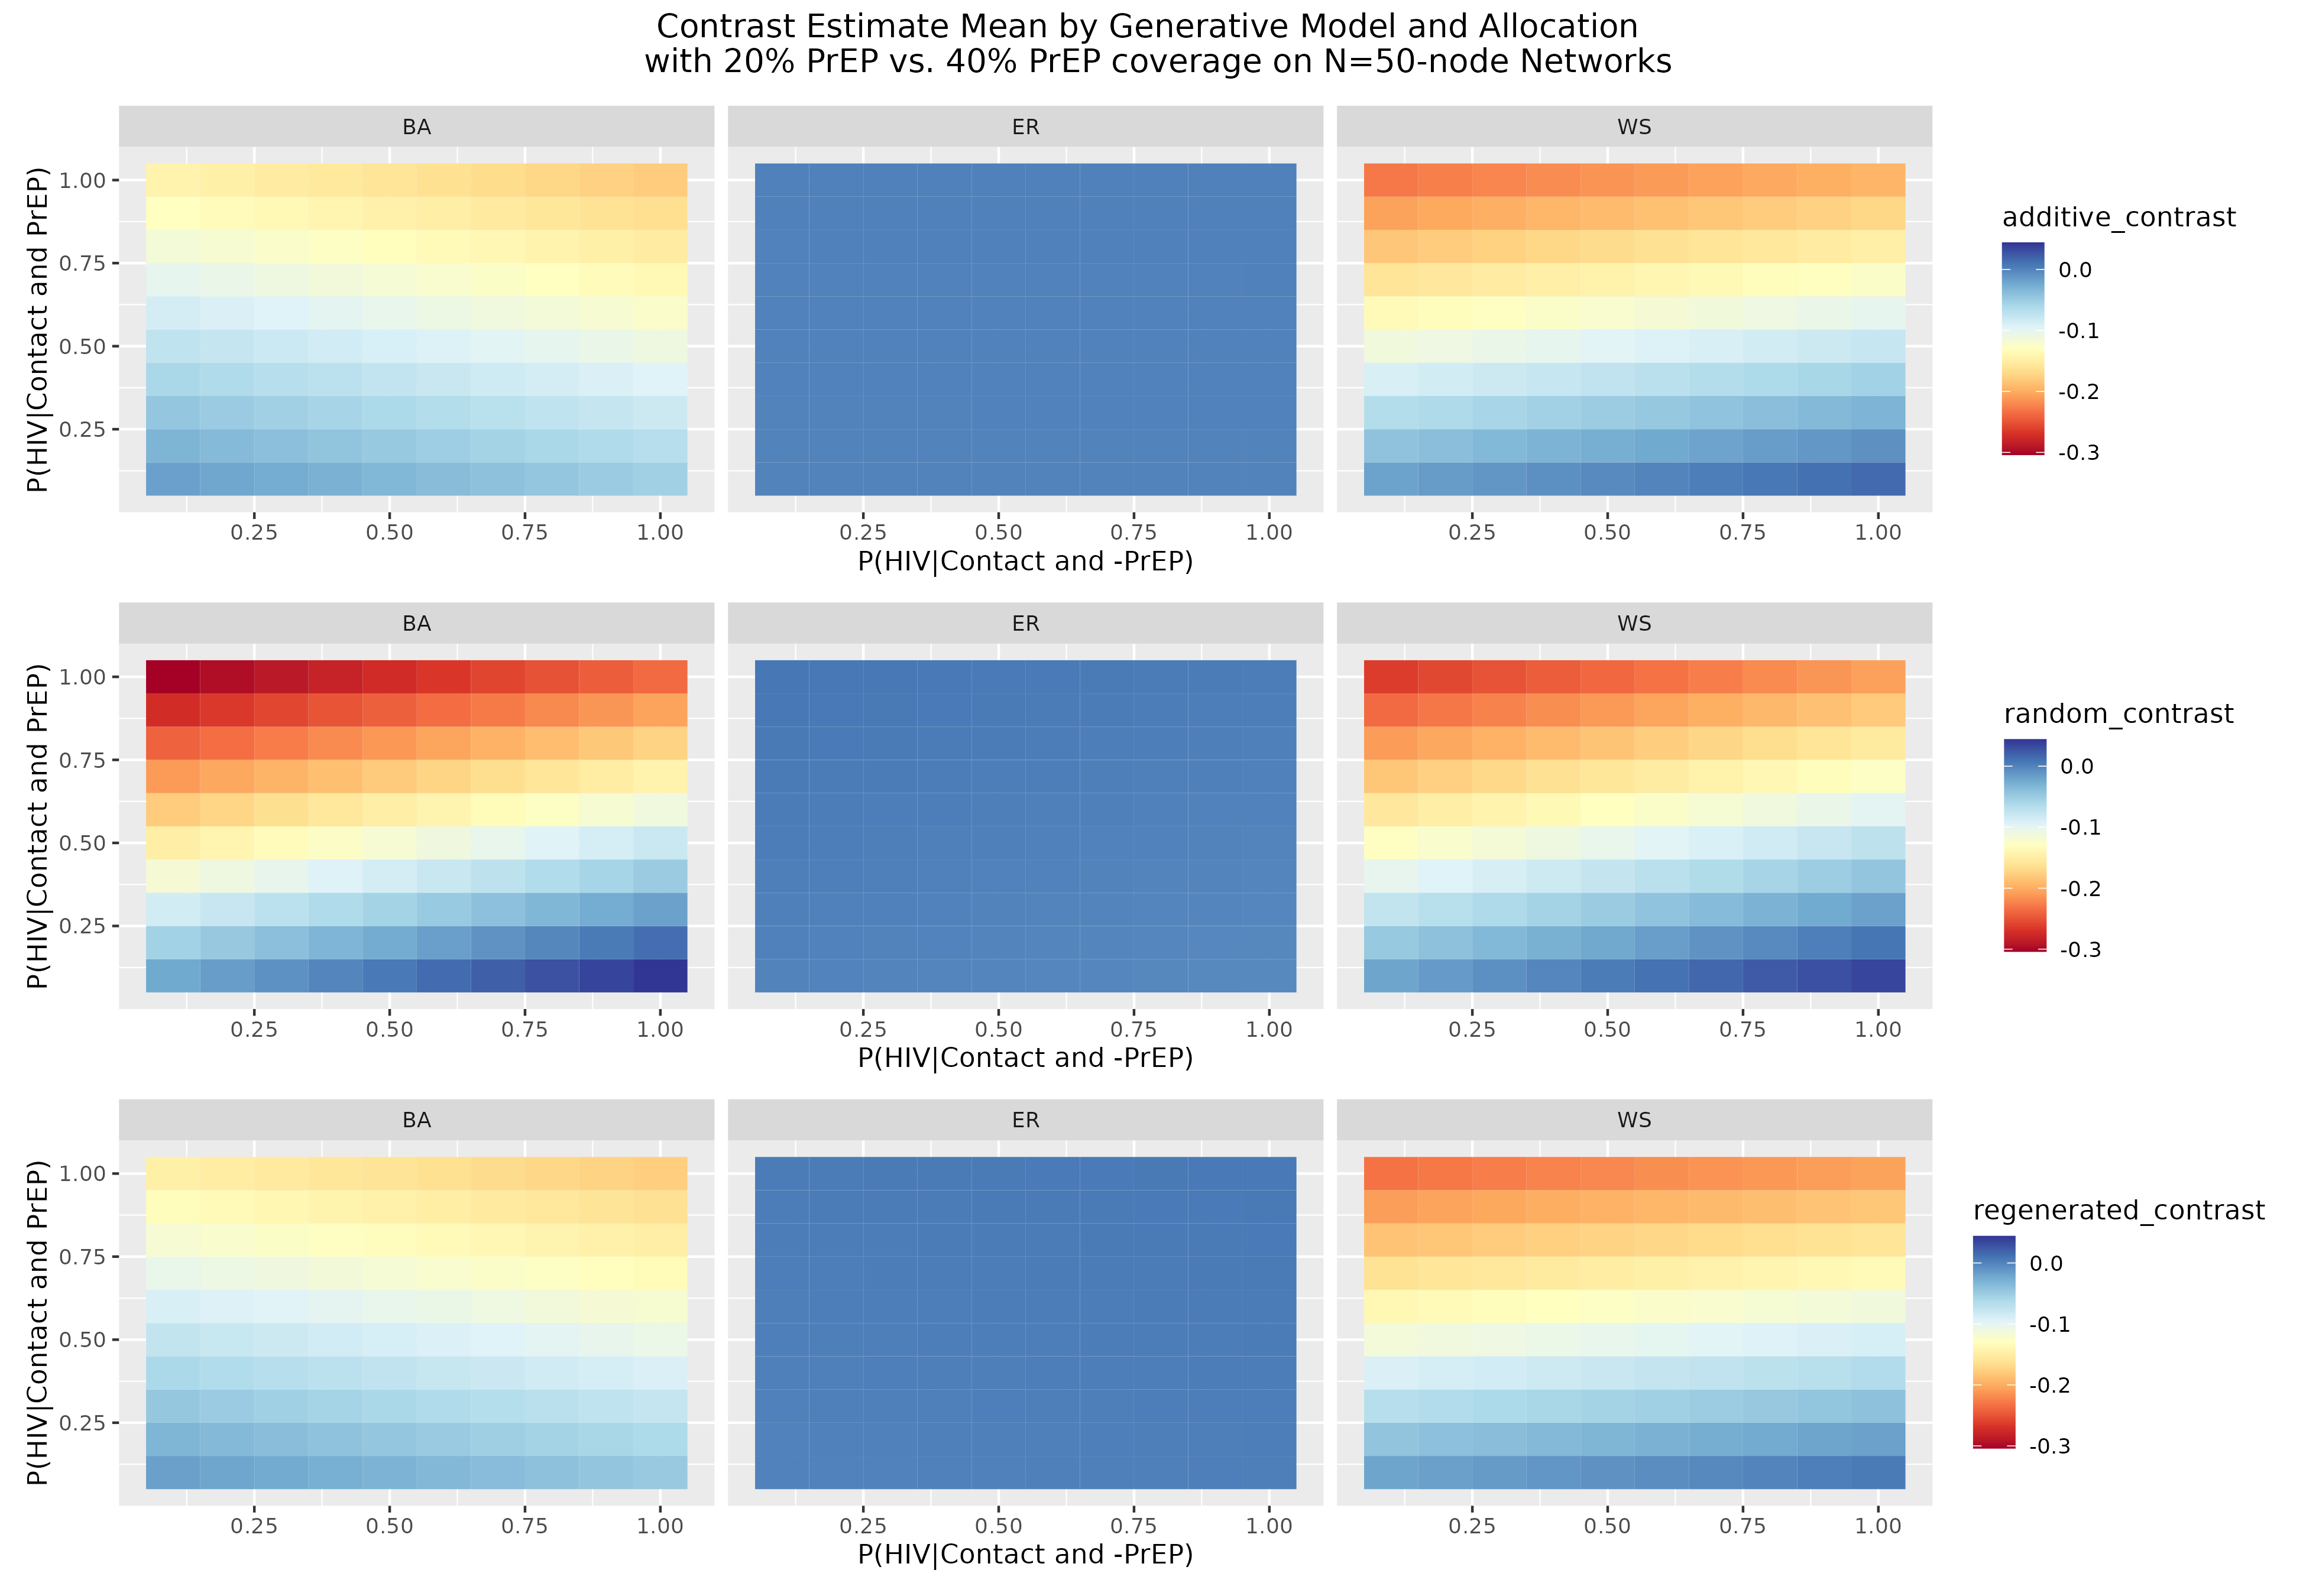
\includegraphics[width=\linewidth]{Corrected Figures/Generative Model Mean Plot.png}
    \caption{Mean of Causal Contrast estimates as $\mathbb{P}\left[\text{HIV} \vert \neg \text{PrEP} \cap \text{Contact}\right]$ and $\mathbb{P}\left[\text{HIV} \vert \text{PrEP} \cap \text{Contact}\right]$ increase, stratified by the model used to generate the networks, and by estimator. From left to right, ``BA" the Barabási–Albert scale-free model, ``ER" the Erdős–Rényi Random Graph model, ``WS" the Watts-Strogatz Small-World model. From top to bottom: ``additive" Mean Contrast of random 20\% additional vs. random 20\% PrEP allocation control, ``random" Mean Contrast of random 40\% PrEP allocation vs. random 20\% control, ``regenerated" Mean Contrast of random 40\% allocation on regenerated network vs. random 20\% control. }
    \label{fig:Figure S4.17}
\end{figure}
From the Causal Contrast Mean plots in Figure \ref{fig:Figure S4.17} above, we can see stark effect modification of the relationship between underlying HIV risks and treatment strategy by the choice of network generative model. In particular, the ER model displays a completely different gradient than those of the BA or WS models for all treatment strategies. There is also a ``reversal" in the direction of effects for the BA model with random allocation compared to additive and regenerated strategies, as well as relatively large differences in magnitude of effect estimates. WS model effect estimate magnitudes are also different across treatment strategies. 

\begin{figure}[H]
    \centering
    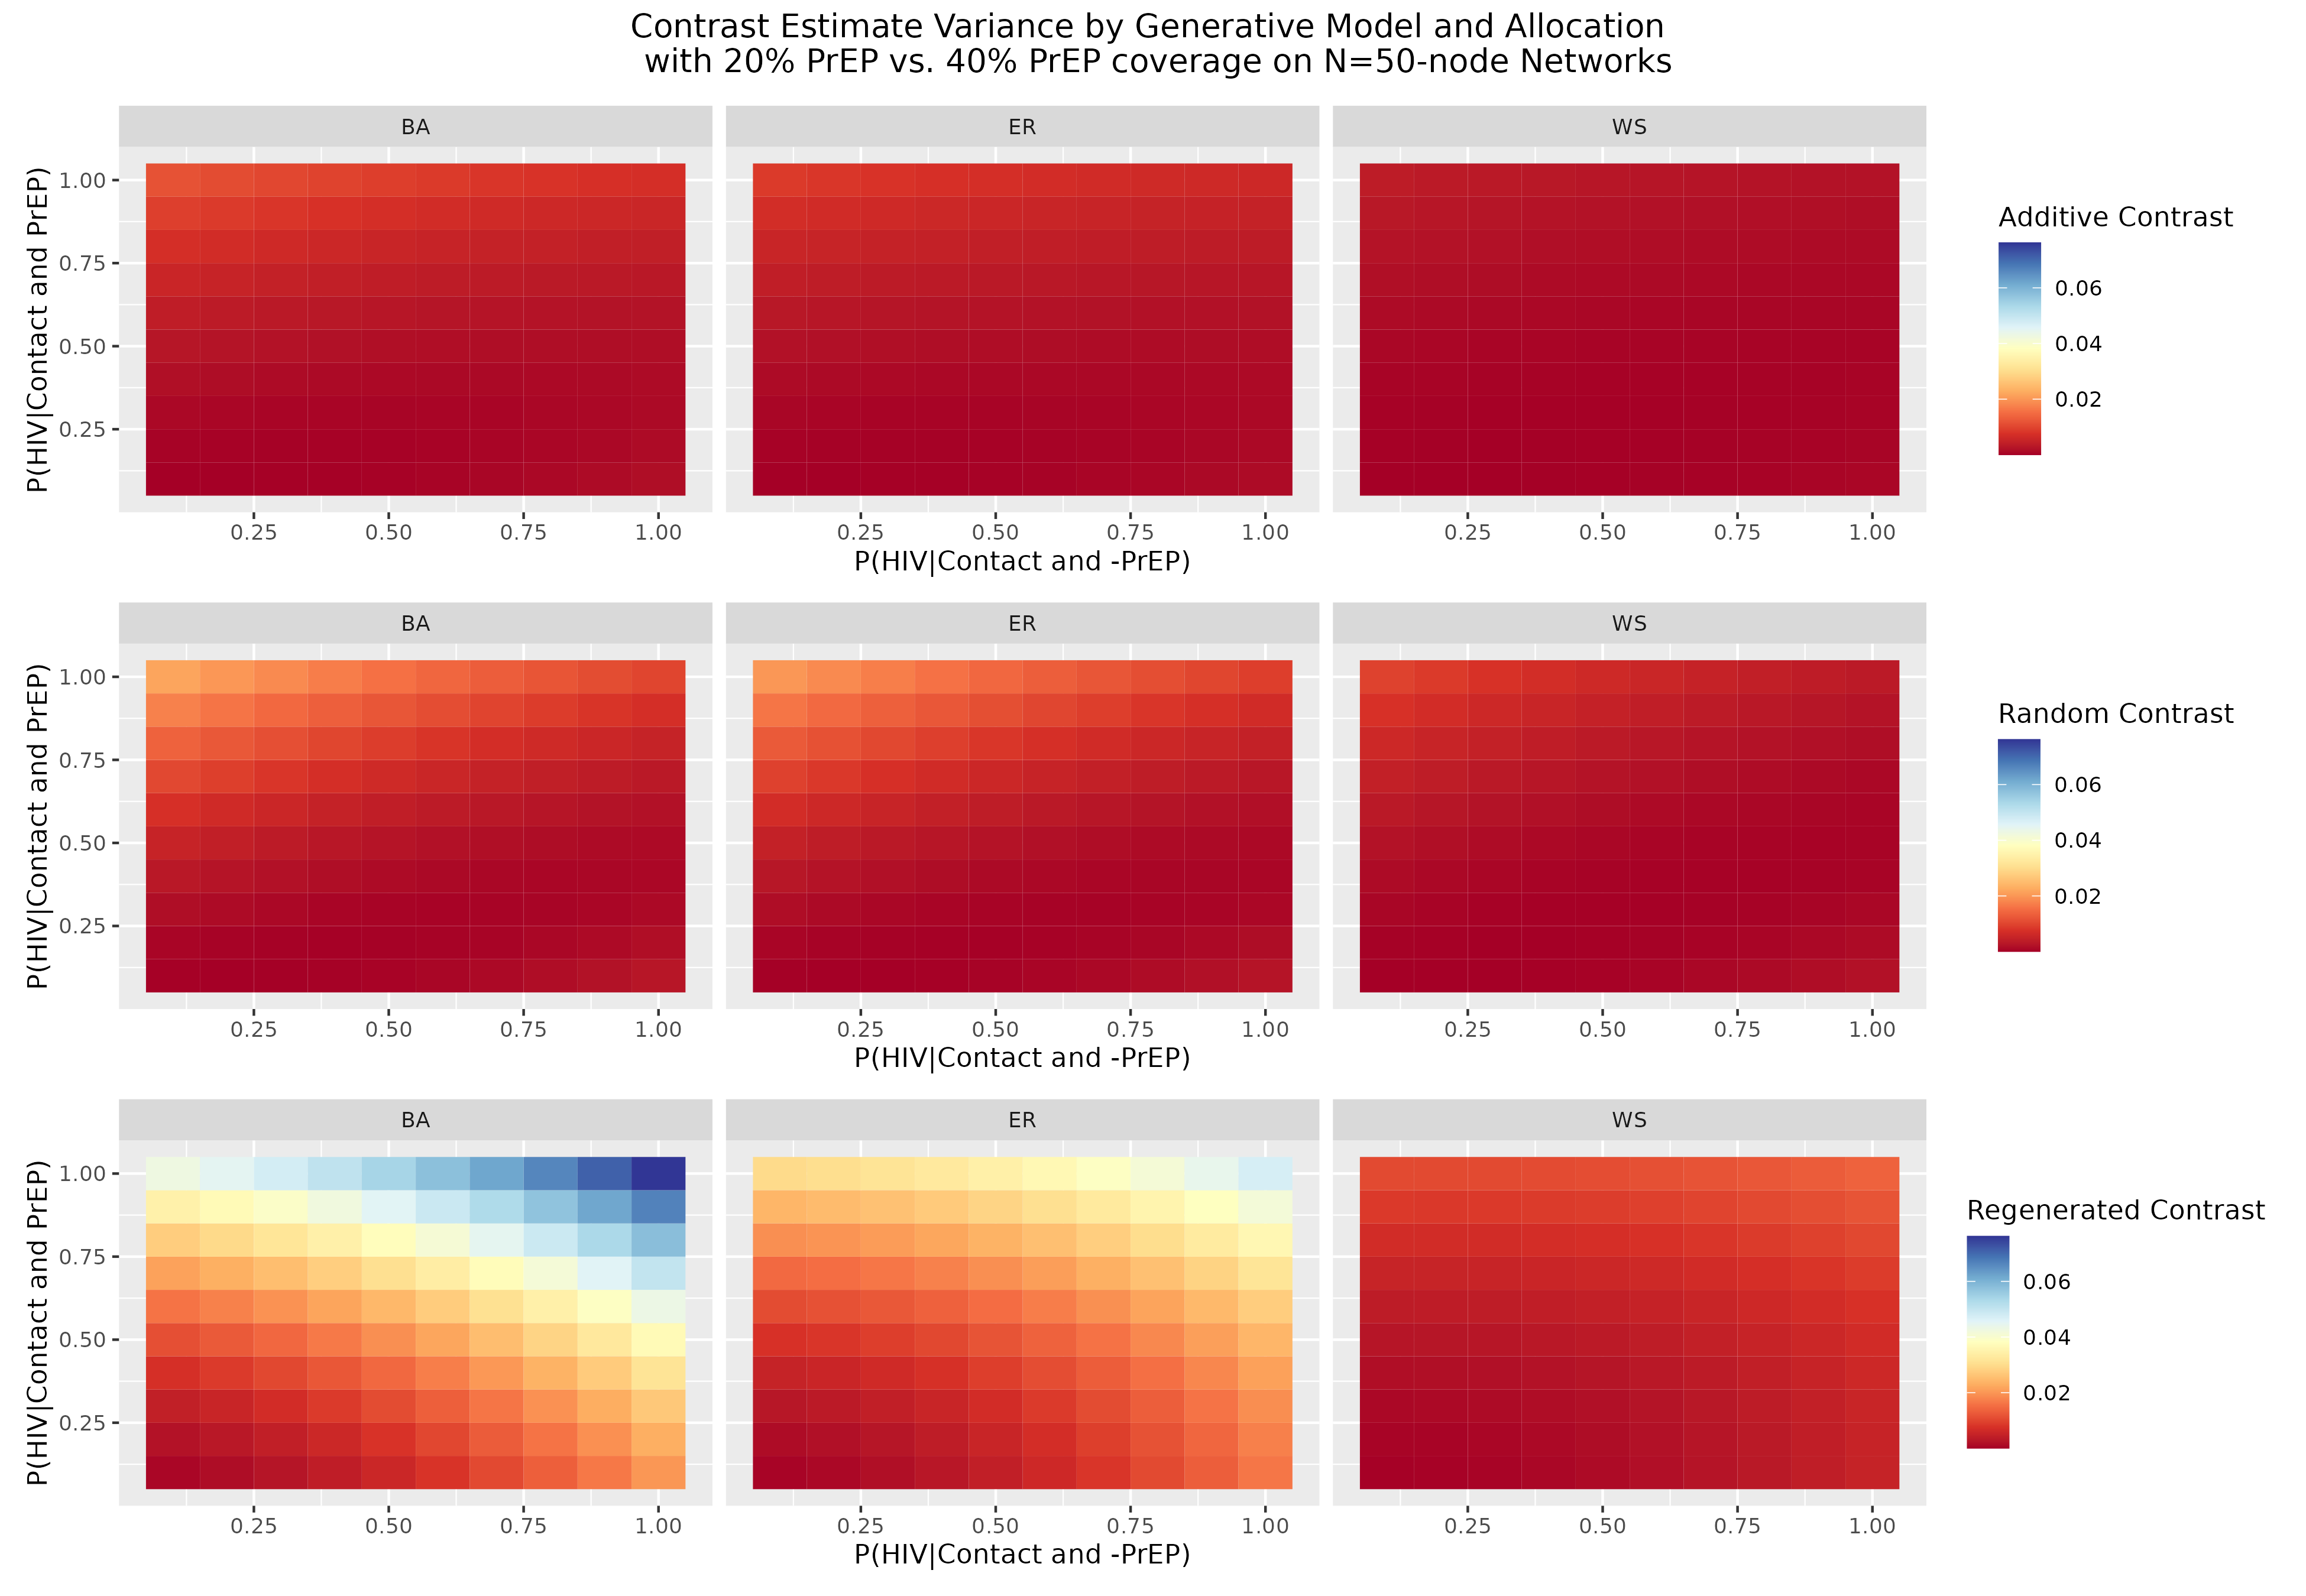
\includegraphics[width=\linewidth]{Corrected Figures/Generative Model Variance Plot.png}
    \caption{Variance of Causal Contrast estimates as $\mathbb{P}\left[\text{HIV} \vert \neg \text{PrEP} \cap \text{Contact}\right]$ and $\mathbb{P}\left[\text{HIV} \vert \text{PrEP} \cap \text{Contact}\right]$ increase, stratified by stratified by the model used to generate the networks, and by estimator. From left to right, ``BA" the Barabási–Albert scale-free model, ``ER" the Erdős–Rényi Random Graph model, ``WS" the Watts-Strogatz Small-World model. From top to bottom: ``additive" Variance of Contrast of random 20\% additional vs. random 20\% PrEP allocation control, ``random" Variance of Contrast of random 40\% PrEP allocation vs. random 20\% control, ``regenerated" Variance of Contrast of random 40\% allocation on regenerated network vs. random 20\% control.}
    \label{fig:Figure S4.18}
\end{figure}
The Causal Contrast Variance plots in Figure \ref{fig:Figure S4.18} above also clearly show the differing results by the choice of network generative model.  Interestingly, the Variance gradients appear similar across models in the ``additive" allocation strategy. While the magnitudes of Variance estimates vary slightly, the gradient for the Watts-Strogatz model is much more consistent  across allocation strategies than for the Barabási–Albert or  Erdős–Rényi models. In particular, the gradients within these two models are markedly different by allocation strategy, although the pattern of changes is similar between these models across strategies. 


\end{document}